\documentclass[11pt,titlepage]{report}
\usepackage{Preamble}
\addbibresource{ref.bib}

\begin{document}

\begin{titlepage}
	\newgeometry{margin=3cm}
	\centering
    
\includegraphics[width=0.6\linewidth]{hes/hei}\\[1cm] 	% University Logo
    \textsc{\LARGE Haute école d'ingénieur du Valais}\\ \vspace{\fill}
    
\includegraphics[width=1\linewidth]{Images/Logo_LoRaSnow.png}\\ \vspace{\fill}
	%\textbf{\textsc{\fontsize{35}{35}\selectfont LoRaSnow}}\\ \vspace{\fill}
	\textsc{\LARGE Mesure du niveau de neige en conditions difficiles}\\[0.4cm]
	\rule{\linewidth}{0.2 mm} \\[0.5 cm]
	Samy Francelet \\
	\today
\end{titlepage}
\restoregeometry

\tableofcontents
\listoffigures
\listoftables
\pagestyle{fancy}

\chapter{Introduction}
\begin{summary}
\section{Contexte}

Ne vous est-il jamais arrivé de vous réveiller un matin et, lorsque vous prenez votre véhicule ou un 
transport en commun, surprise ! Il a neigé durant la nuit, et les services de déneigement n'y étaient
visiblement pas préparés.\\
LoRaSnow est un projet qui vise à palier à ce problème. Intégrant les dernières technologies de l'internet 
des objets et une utilisation intelligente de capteurs, ces modules alertent les services privés et
communaux de chutes de neige dès les premiers flocons, permettant une réaction rapide et efficace.\\
En effet, le système d'alerte de piquet en place ne permet pas une vue globale de la région, et tarde
parfois à réagir. De plus, les prévisions météorologiques sont parfois imprécises quand il s'agit de 
quantité de précipitations. Ce projet amène donc une surveillance constante et automatique d'une région,
remplaçant par la même occasion le système coûteux déjà en place.

\end{summary}

\part{Technique}

\chapter{Spécifications}
\section{Cahier des charges}



\section{Schéma bloc global}



\chapter{LiDAR}

\section{Implémentation}
Pour tester les algorithmes de mesure avec des vidéos sur le terrain,
Dr. Mudry Pierre-André et M. Matter Fabien nous on aimablement laissé accès à
la caméra de notre projet parent \emph{VibroSnow\cite{VibroSnow}} et nous
les remercions énormément.

\subsection{Récupération des vidéos}
La caméra de \emph{VibroSnow} détecte le passage d'objet (voitures, chute de neige,...) et
enregistre une vidéo qui est ensuite transmise à un serveur \emph{Windows}.
Bien que l'accès aux vidéos nous a été donné, nous ne pouvons pas aller chercher les vidéos
directement sur le serveur \emph{Windows} car il est utilisé pour d'autres projets auxquels nous
n'avons pas accès.\\
Il a donc fallu créer un script \emph{Powershell}, transferant chaque jour les vidéos
cumulées sur le serveur \emph{Windows} vers un serveur auquel nous avons accès.
Un \emph{Raspberry Pi} a été mis en place comme serveur pour récuperer les vidéos.

\subsection{Mesure du débit de chute de neige}
La méthode utilisée pour détecter les chutes de neige se décompose ainsi :
\begin{description}
    \item[Soustraction de deux images] \hfill \\
    pour isoler les éléments qui ont bougé entre les deux images
    \item[Seuillage des niveaux de blancs sur l'image] \hfill \\
    pour accentuer les chutes de neige
    \item[Calcul du ratio de pixels blancs] \hfill \\
    pour avoir un nombre correspondant au débit de chute de neige    
\end{description}

\begin{figure}[H]
    \begin{subfigure}{.45\textwidth}
        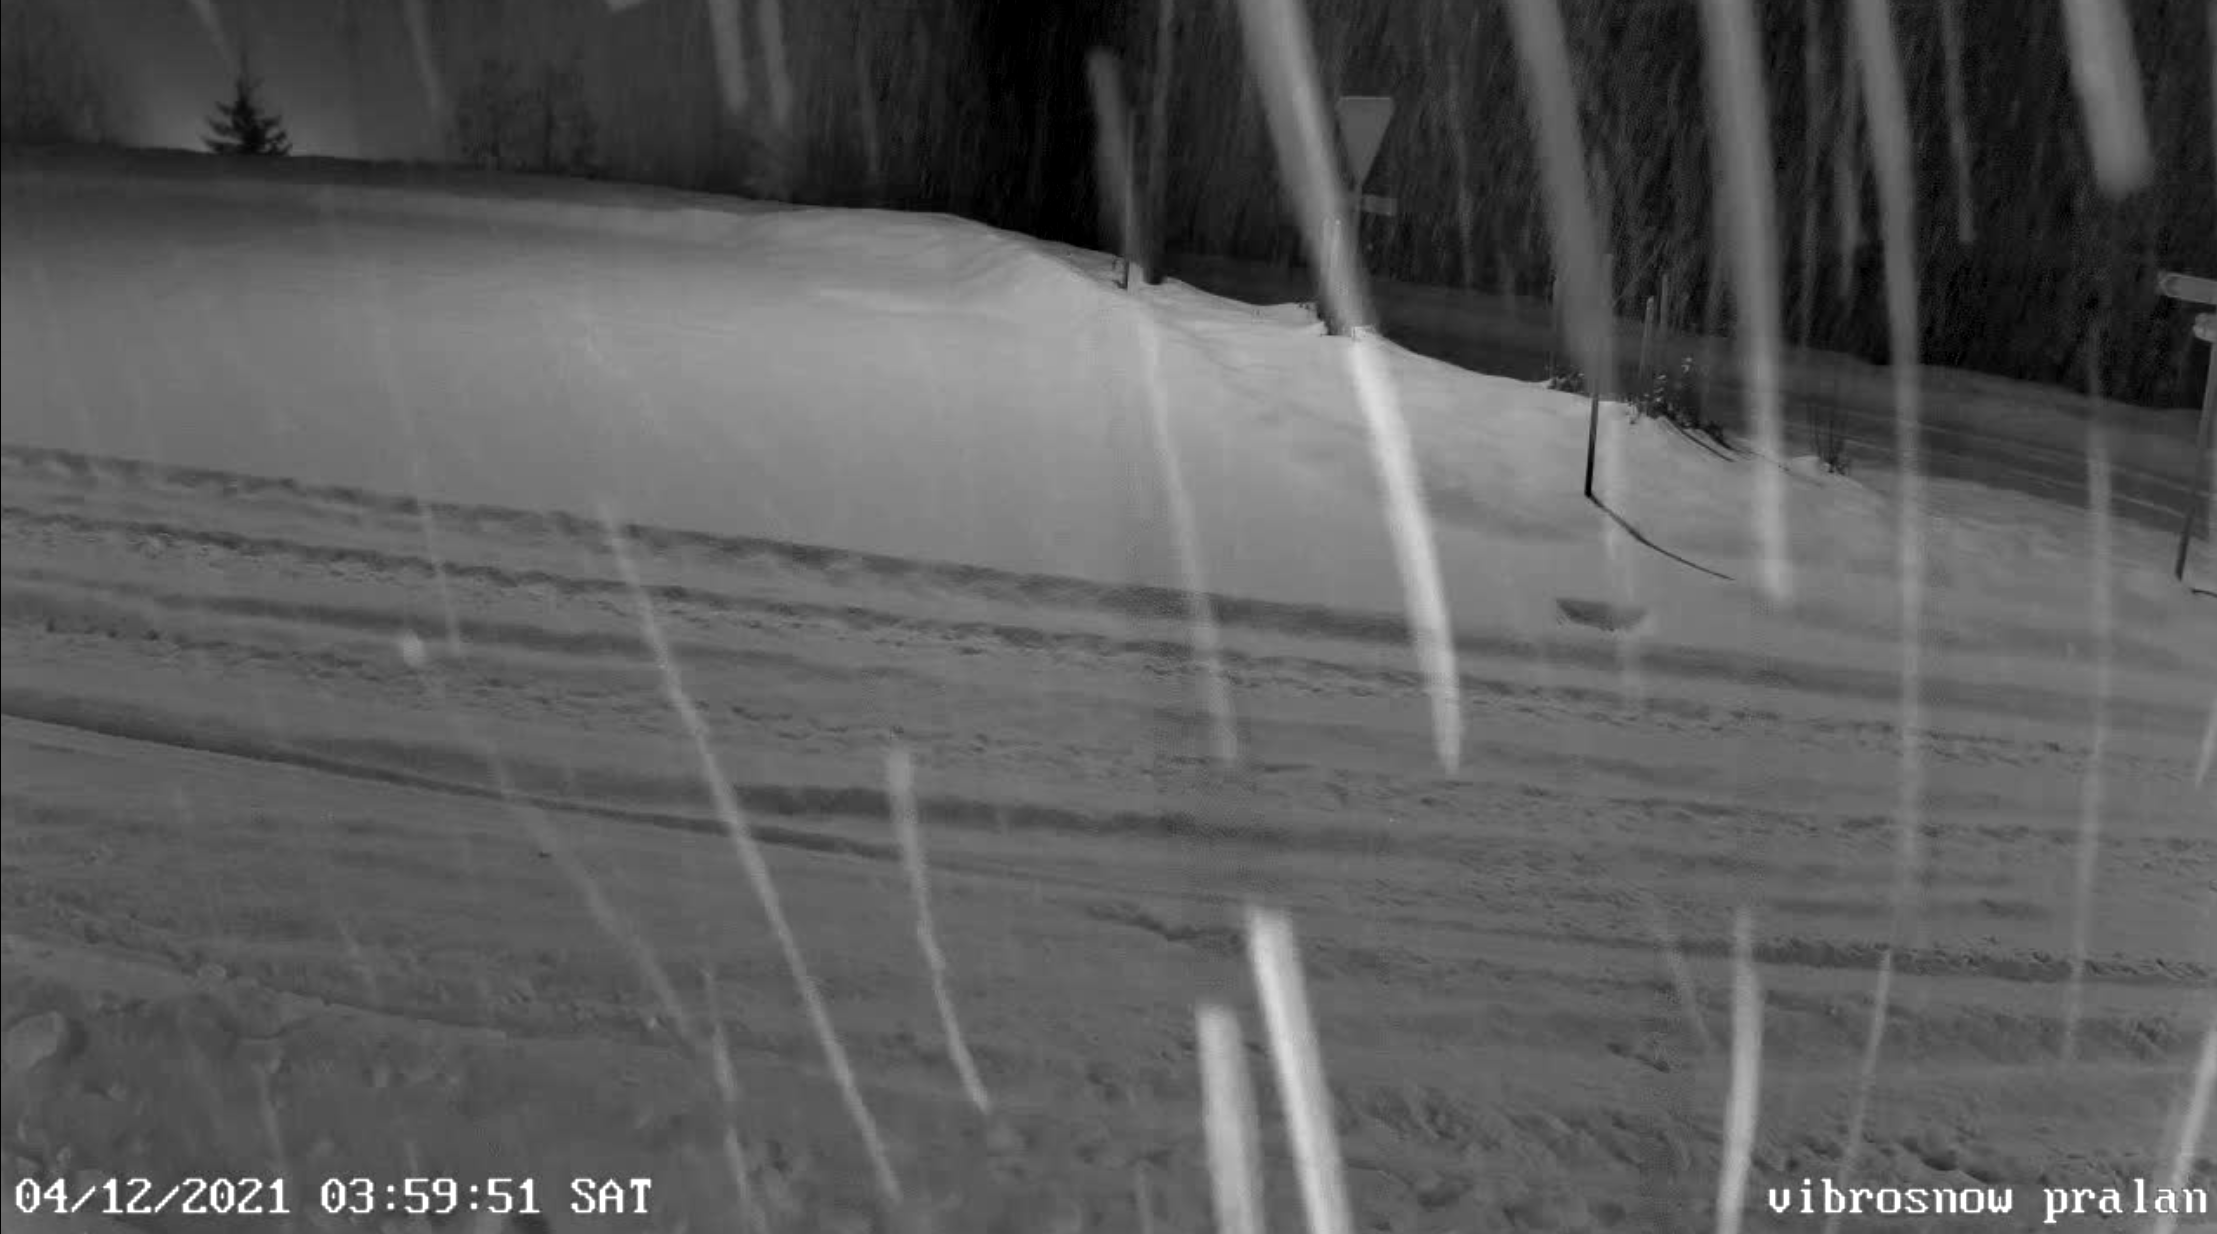
\includegraphics[width=\linewidth]{Images/computer_vision/snowfall/original.png}
        \caption{Image originale}
        \label{fig:Snowfall_original}
    \end{subfigure}
    \hfill
    \begin{subfigure}{.45\textwidth}
        
\includegraphics[width=\linewidth]{Images/computer_vision/snowfall/noise.png}
        \caption{Image avec neige isolée}
        \label{fig:Snowfall_noise}
    \end{subfigure}
    \hfill
    \centering
    \begin{subfigure}{.45\textwidth}
        
\includegraphics[width=\linewidth]{Images/computer_vision/snowfall/snowfall.png}
        \caption{Image seuillée avec calcul du ratio de pixels blancs (9.05\% ici)}
        \label{fig:Snowfall_thres}
    \end{subfigure}
    \caption{Étapes de la mesure de débit de chute de neige}
    \label{fig:Snowfall_algorithm}
\end{figure}
\newpage

\subsection{Détection de route enneigée}
Deux méthodes ont été testées pour détecter si la route est enneigée ou non.\\
La première réalise un simple seuillage des niveaux de blancs, et un calcul
du ratio des pixels blancs sur l'image. On récupère plusieurs images et on
calcul la moyenne du ratio de blanc sur toute les images.
Cette moyenne est ensuite comparée à une moyenne similaire réalisée sur une
vidéo de la route déneigée, en vérifiant qu'on se trouve au même moment de
la journée (jour/nuit, matin/après-midi).\\
La deuxième est identique, à l'exception d'une suppression du bruit réalisée
avant le seuillage. Cette suppresion du bruit reprends la méthode d'isolation
de neige utilisée pour mesurer le débit de chute de neige et soustrait cette image
de bruit à l'image originale. Cette méthode demande un peu plus de calculs mais peut
potentiellement générer un résultat plus fiable.

\begin{figure}[H]
    \begin{subfigure}{.45\textwidth}
        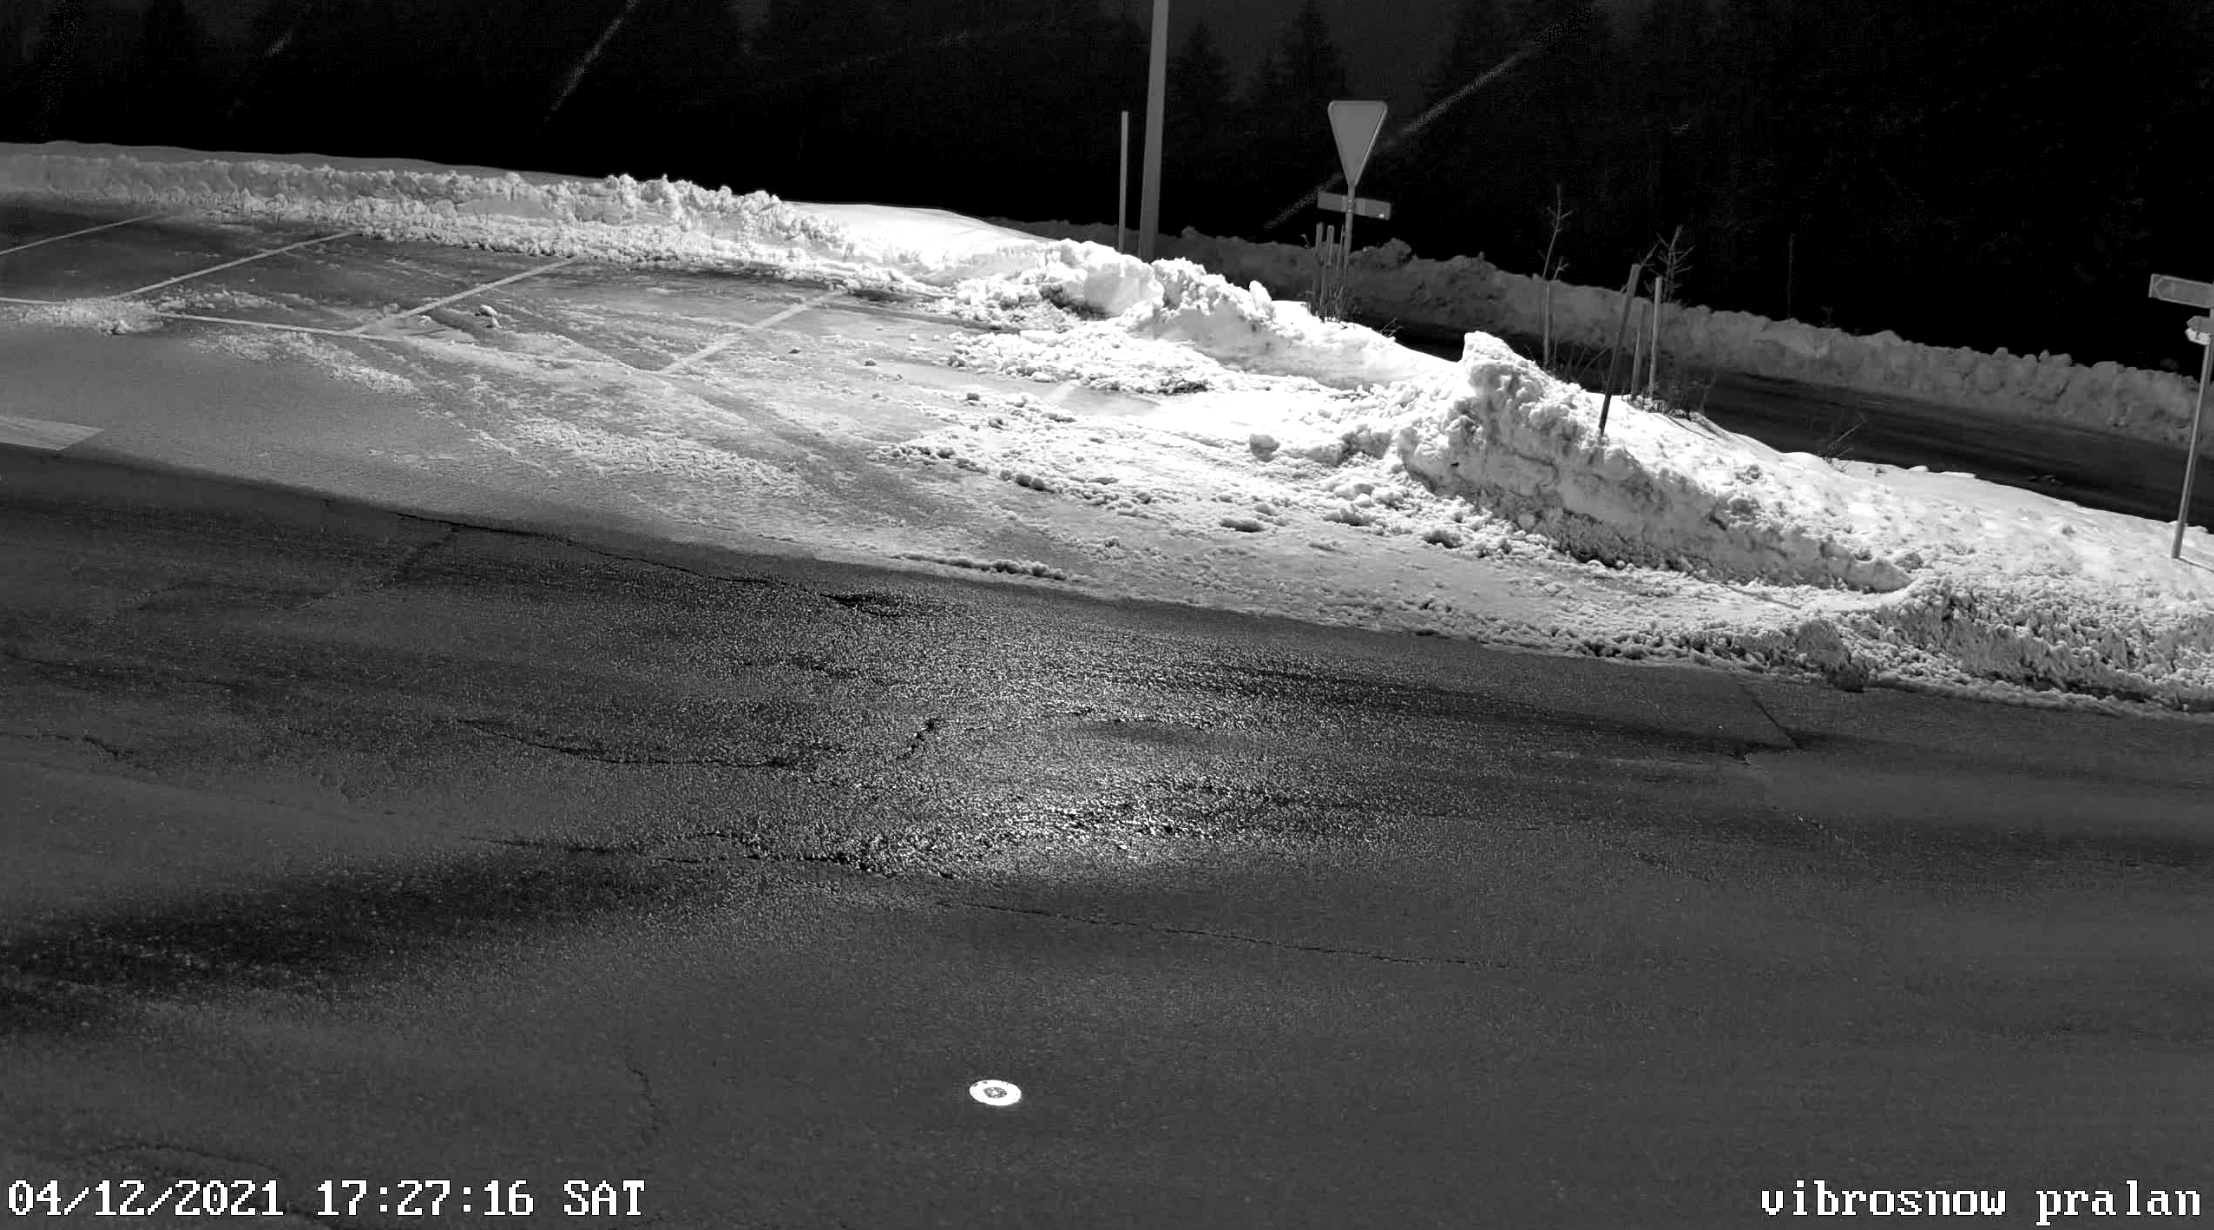
\includegraphics[width=\linewidth]{Images/computer_vision/snowOnRoad/ref_original.png}
        \caption{Image de référence originale}
        \label{fig:SnowOnRoad_ref_original}
    \end{subfigure}
    \hfill
    \begin{subfigure}{.45\textwidth}
        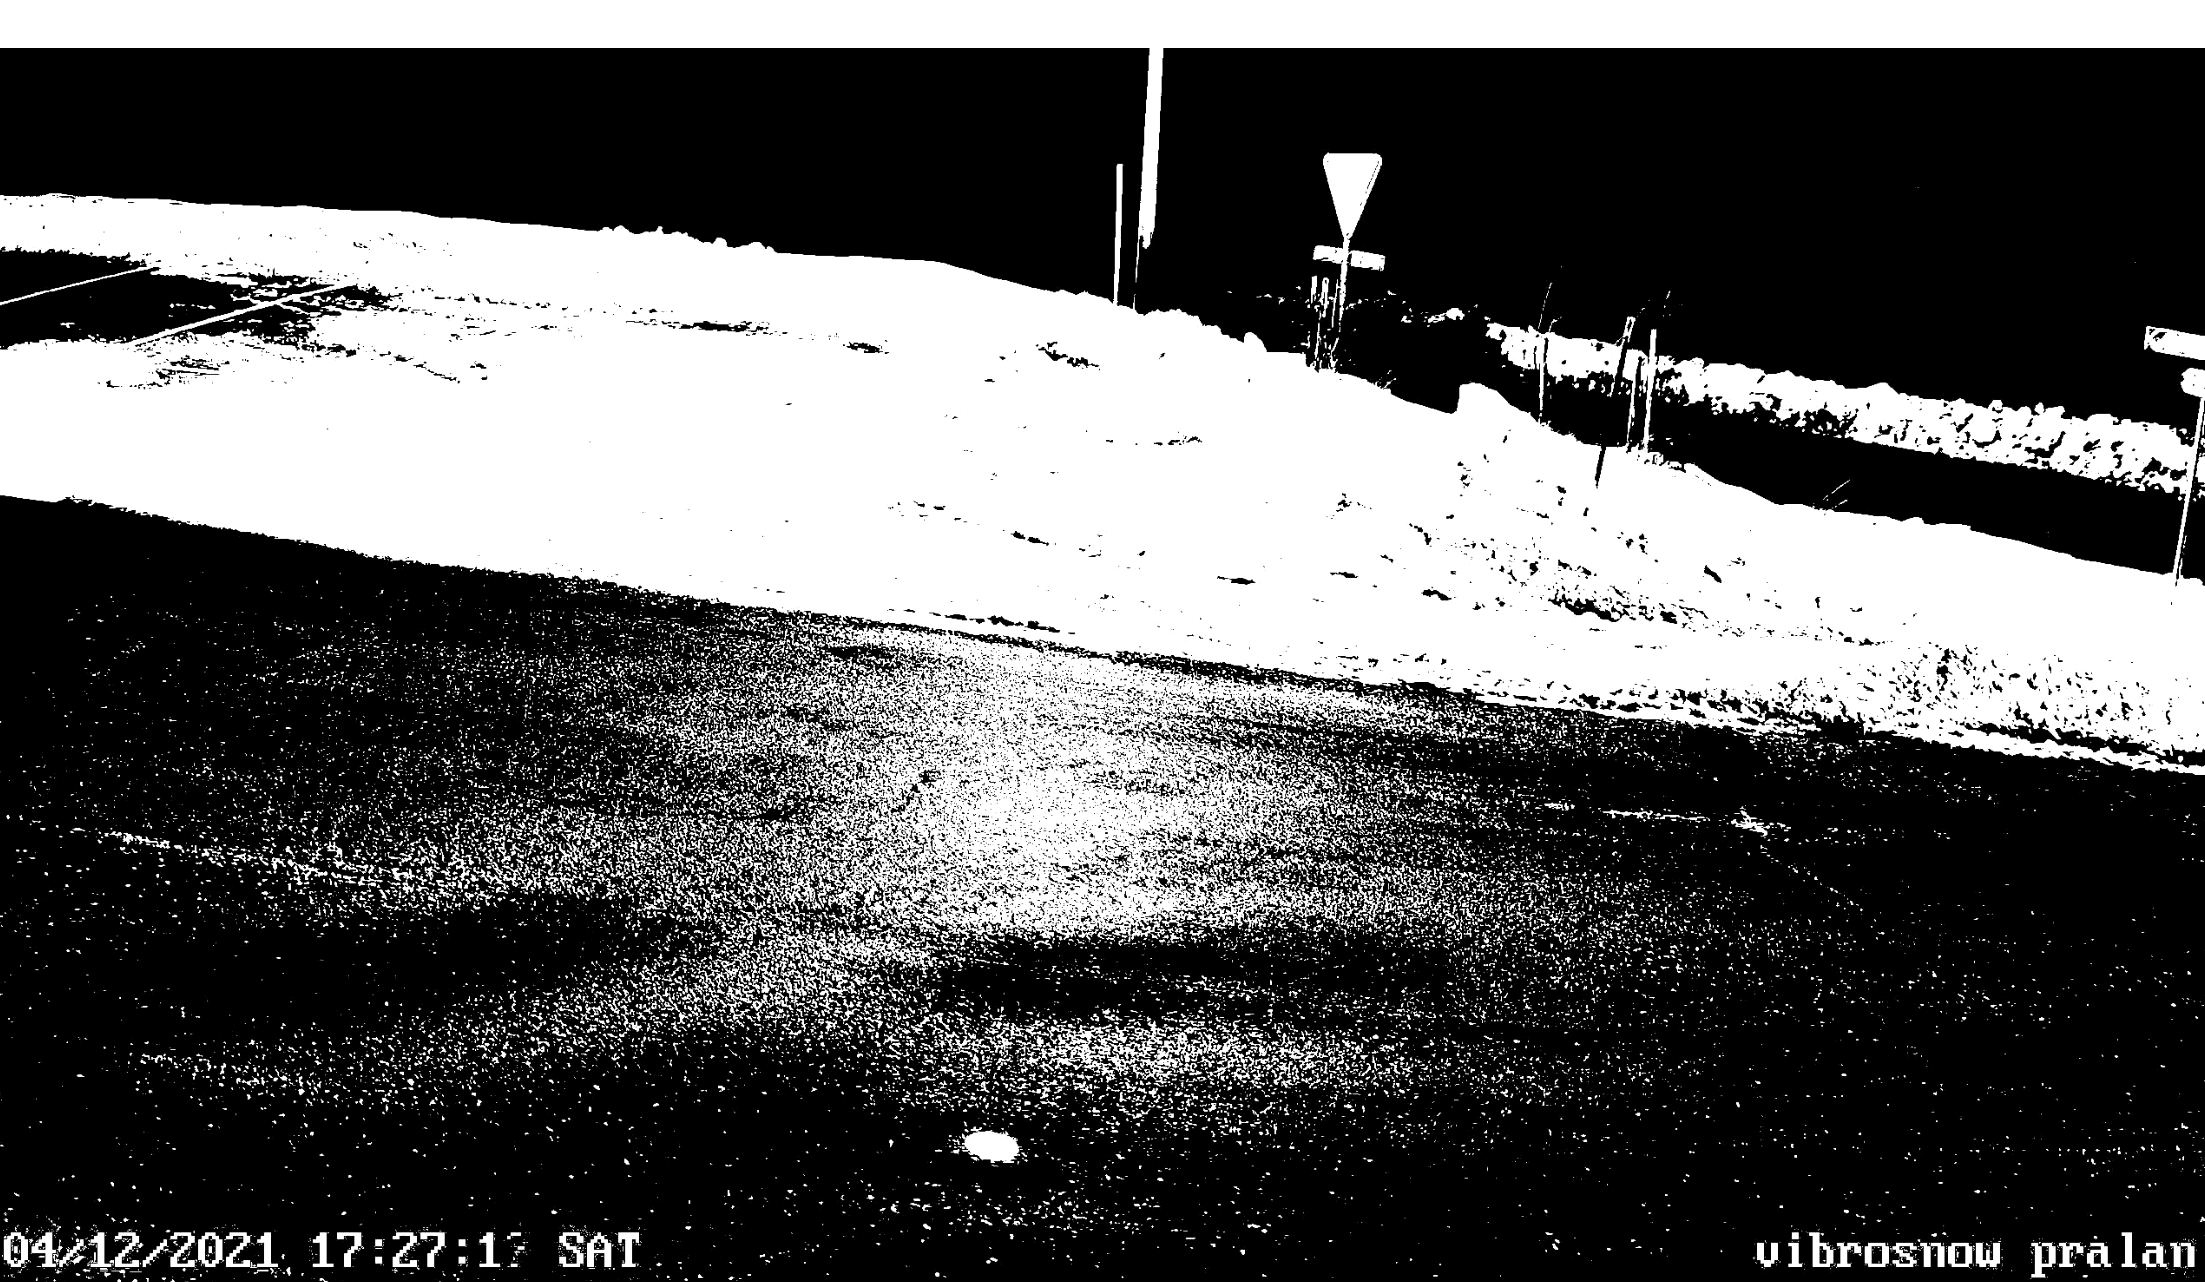
\includegraphics[width=\linewidth]{Images/computer_vision/snowOnRoad/ref_thres.png}
        \caption{Image de référence seuillée}
        \label{fig:SnowOnRoad_ref_thres}
    \end{subfigure}
    \caption{Image de référence}
    \label{fig:SnowOnRoad_ref}
\end{figure}

\begin{figure}[H]
    \begin{subfigure}{.45\textwidth}
        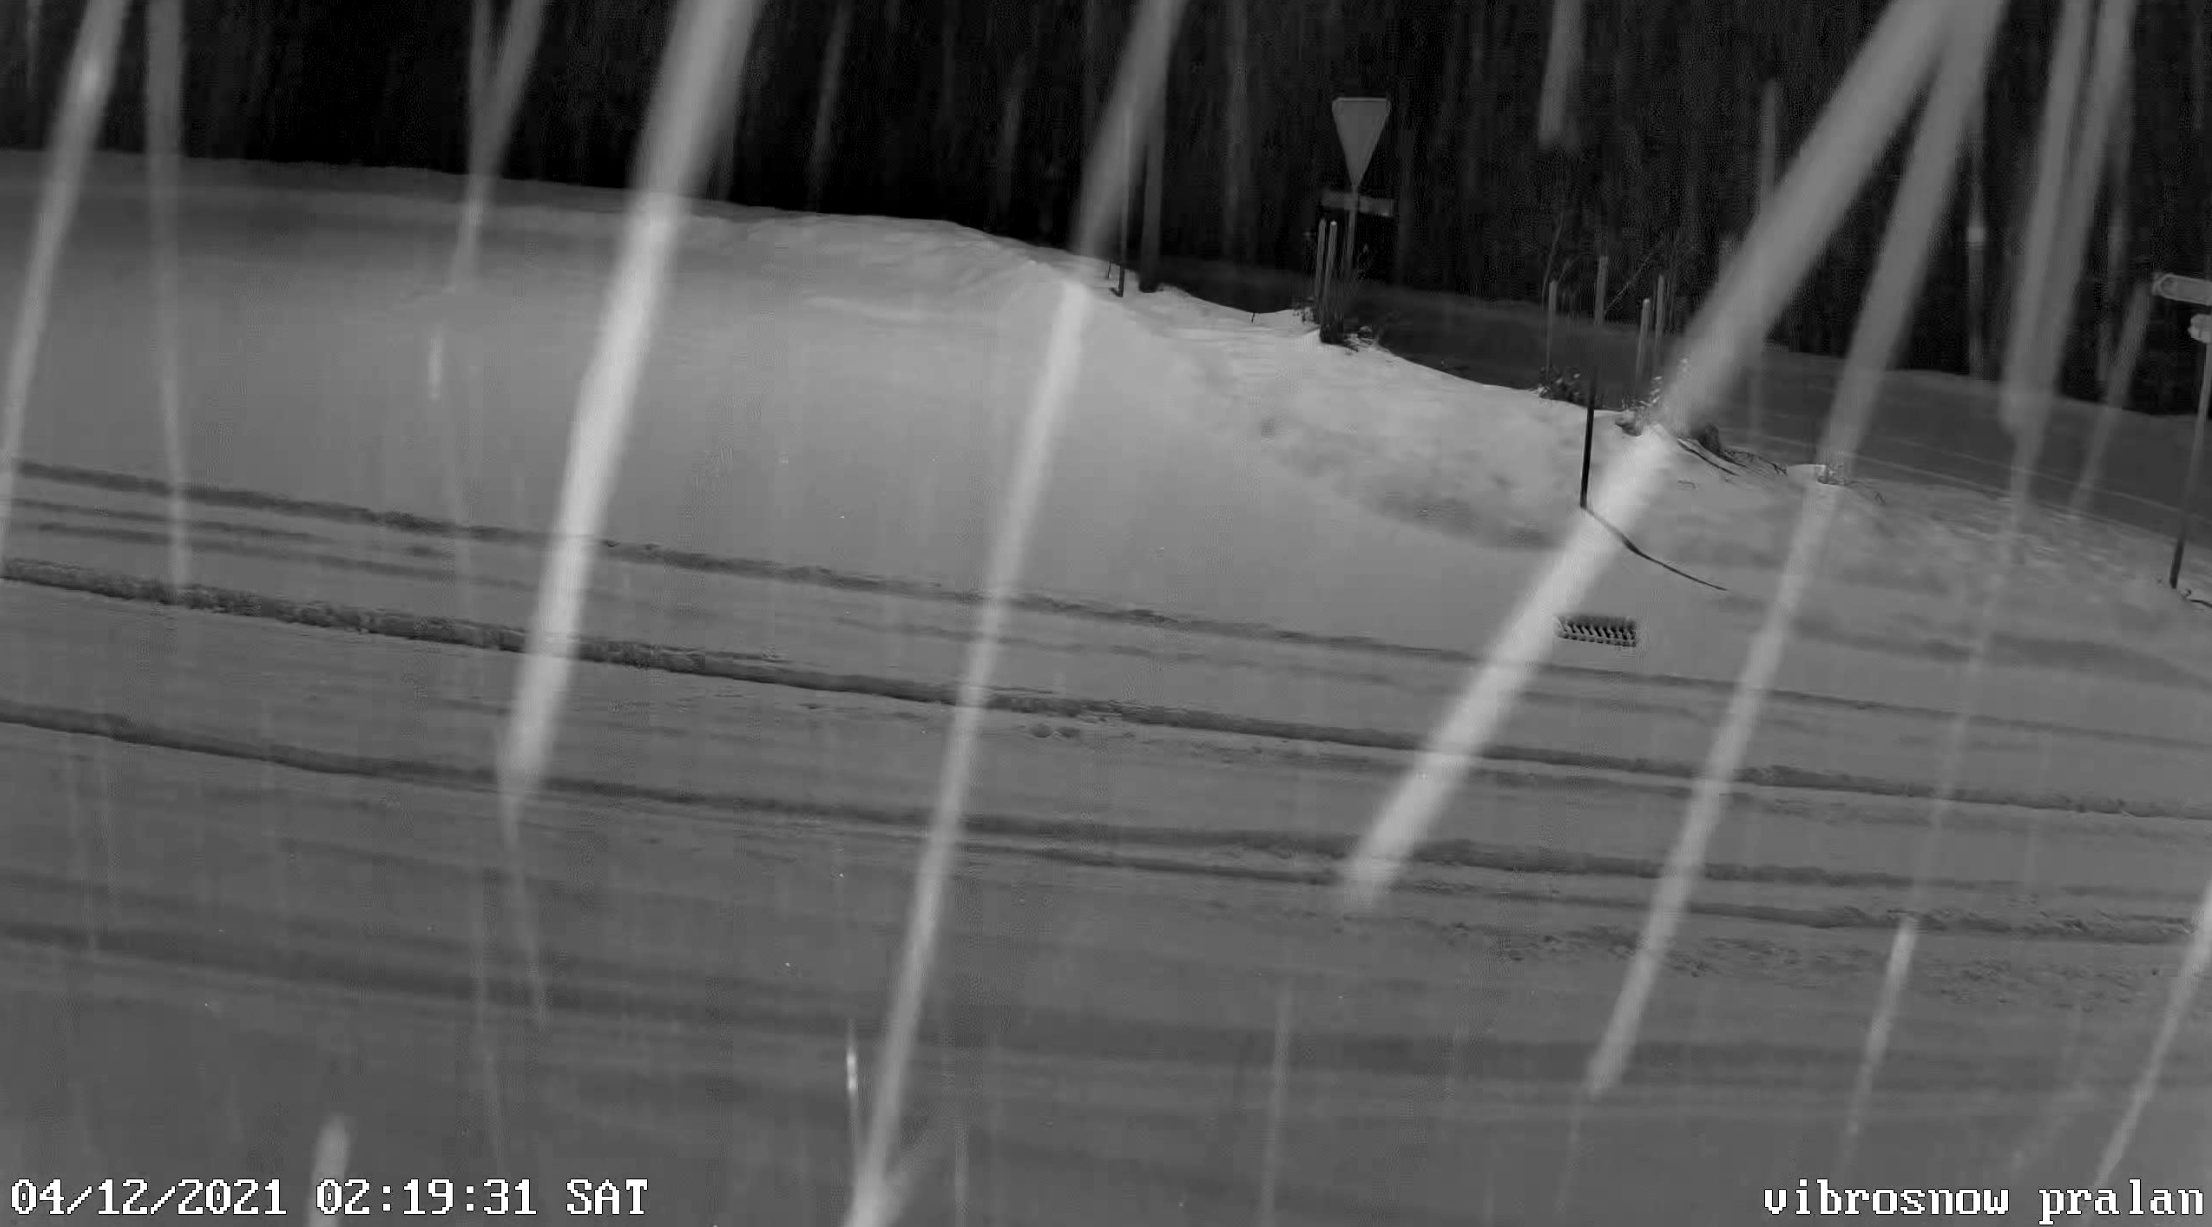
\includegraphics[width=\linewidth]{Images/computer_vision/snowOnRoad/test_original.png}
        \caption{Image de test originale}
        \label{fig:SnowOnRoad_test_original}
    \end{subfigure}
    \hfill
    \begin{subfigure}{.45\textwidth}
        
\includegraphics[width=\linewidth]{Images/computer_vision/snowOnRoad/test_thres.png}
        \caption{Image de test seuillée}
        \label{fig:SnowOnRoad_test_thres}
    \end{subfigure}
    \hfill
    \begin{subfigure}{.45\textwidth}
        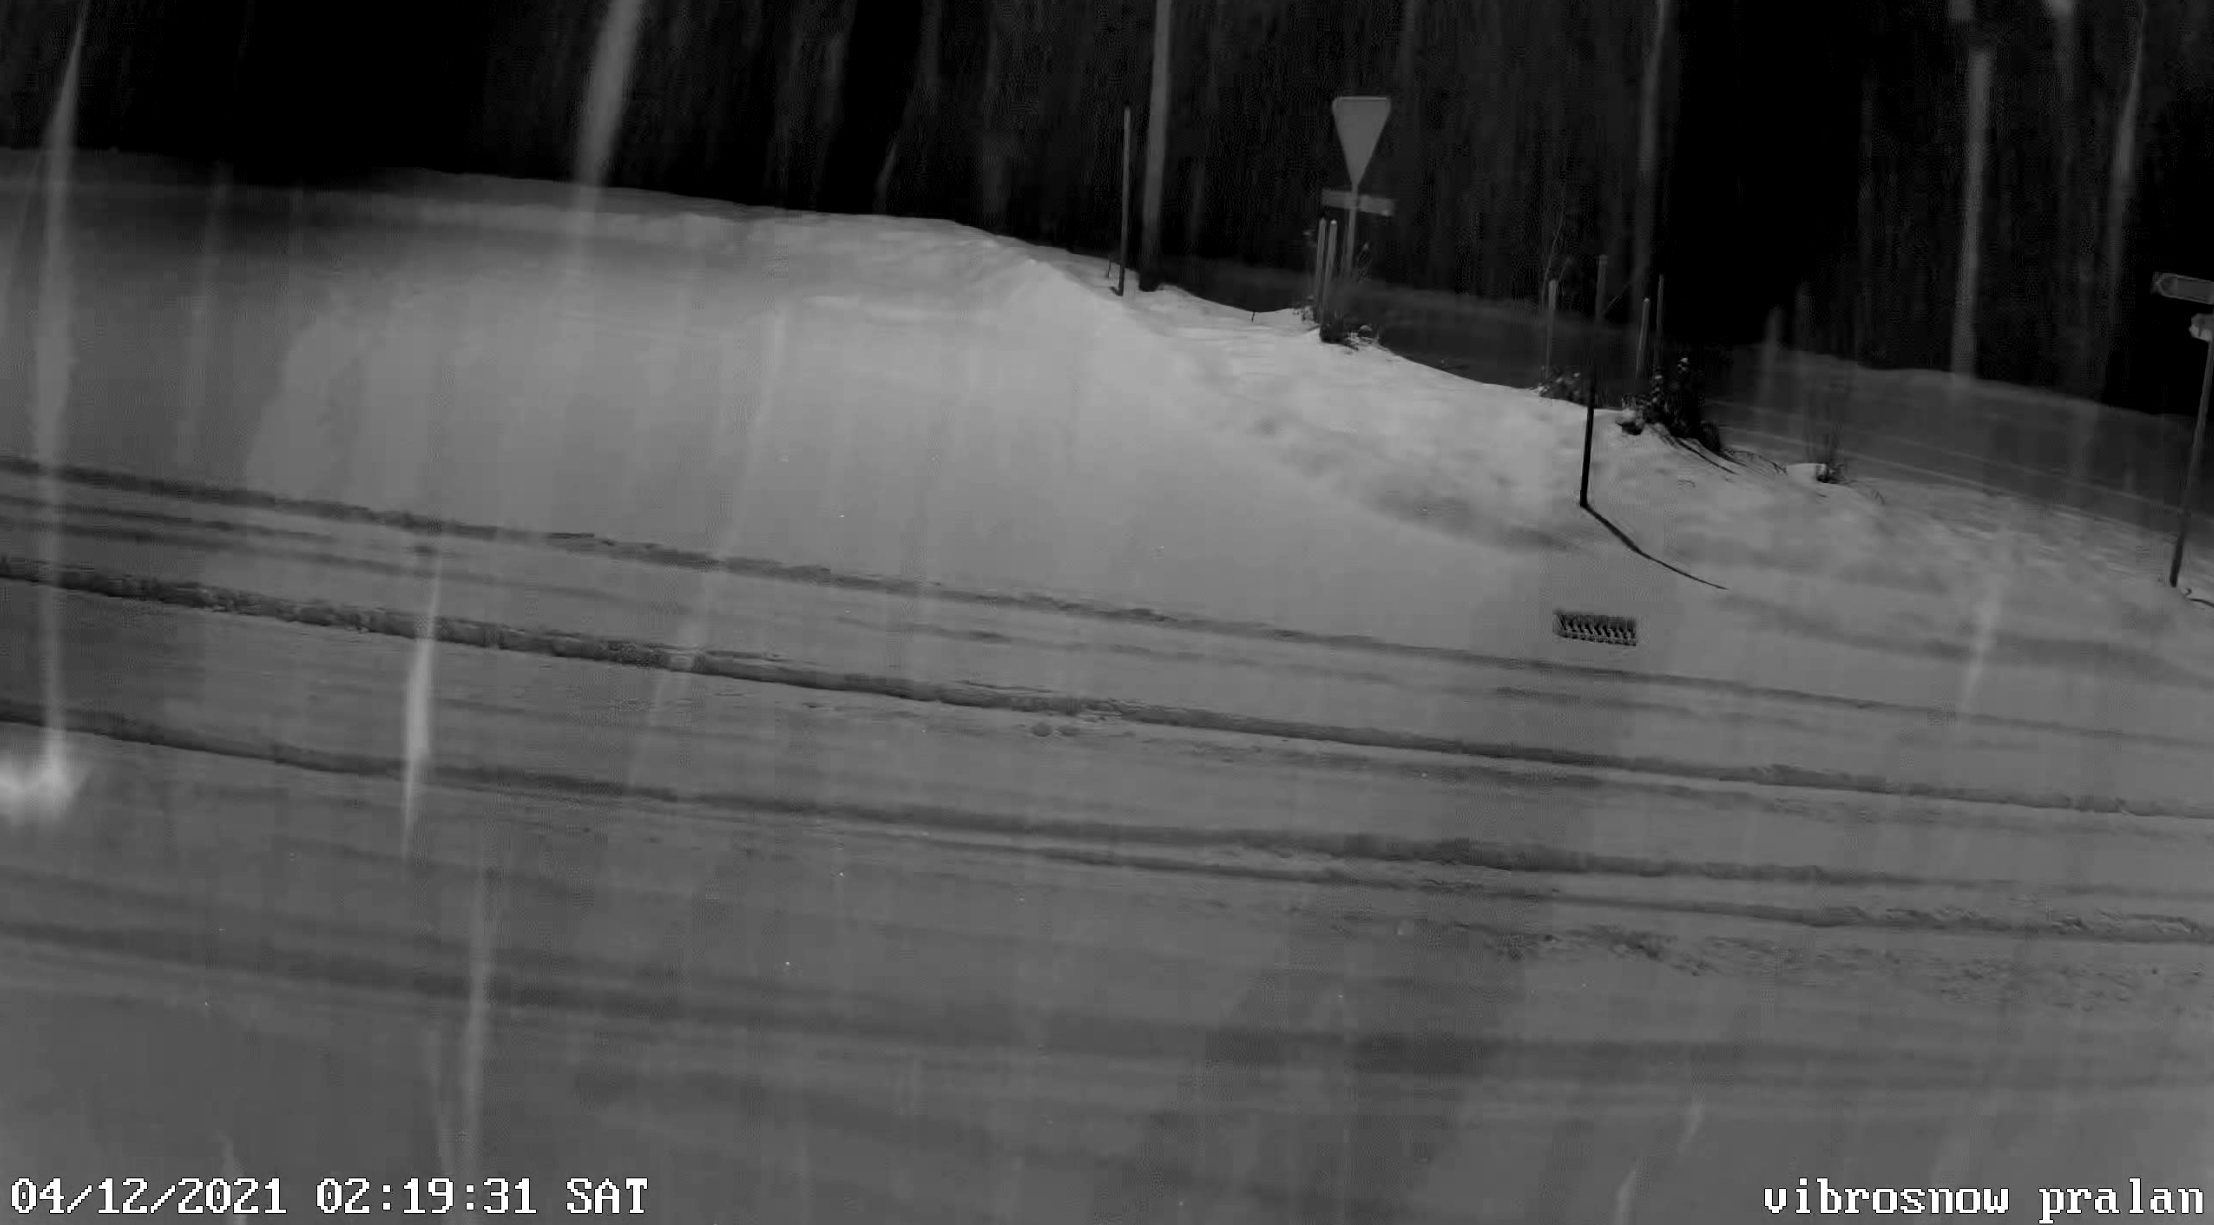
\includegraphics[width=\linewidth]{Images/computer_vision/snowOnRoad/test_denoised.png}
        \caption{Image de test avec suppression de bruit}
        \label{fig:SnowOnRoad_test_denoised}
    \end{subfigure}
    \hfill
    \begin{subfigure}{.45\textwidth}
        
\includegraphics[width=\linewidth]{Images/computer_vision/snowOnRoad/test_denoisedThres.png}
        \caption{Image de test avec suppression de bruit et seuillée}
        \label{fig:SnowOnRoad_test_denoisedThres}
    \end{subfigure}
    \caption{Image de test}
    \label{fig:SnowOnRoad_test}
\end{figure}
\newpage
\section{Résultats}

Ici seront présentés les résultats des tests qui concernent le LiDAR Lite V4. Au fur et à mesure des
résultats, quelques conclusions seront d'ores et déjà tirées.\\
En annexe, se trouve le protocole de test complet du capteur.

\subsection{Caractéristique de l'erreur de mesure}

Le premier test consiste à mesurer une distance connue avec le capteur et de noter sa valeur mesurée
afin de vérifier si la plage de mesure donnée par la fiche technique (5cm à 10m) est vraie.\\
Ceci nous permet de savoir dans quelle mesure la distance fournie par le capteur représente la réalité.
Dans le cas d'une erreur de mesure, il nous est aussi utile de savoir si cette erreur est constante 
entre plusieurs séries espacées dans le temps.

\subsubsection{Méthode}

Pour ce faire, le capteur a été placé le long d'un étalon gradué de 6 mètres. Un objet est ensuite
placé à un interval de 20cm pour le premier mètre, puis à un interval de 50cm. À chaque mesure, on 
note la valeur mesurée par le LiDAR ainsi que la distance réelle.\\
Cela nous permet donc de comparer la plage de mesure effective du capteur, dans les tolérences
annoncées. La figure \ref{fig:RealDistanceMeasures} montre la mise en place du test de distance.

\begin{figure}[H]
    \centering
    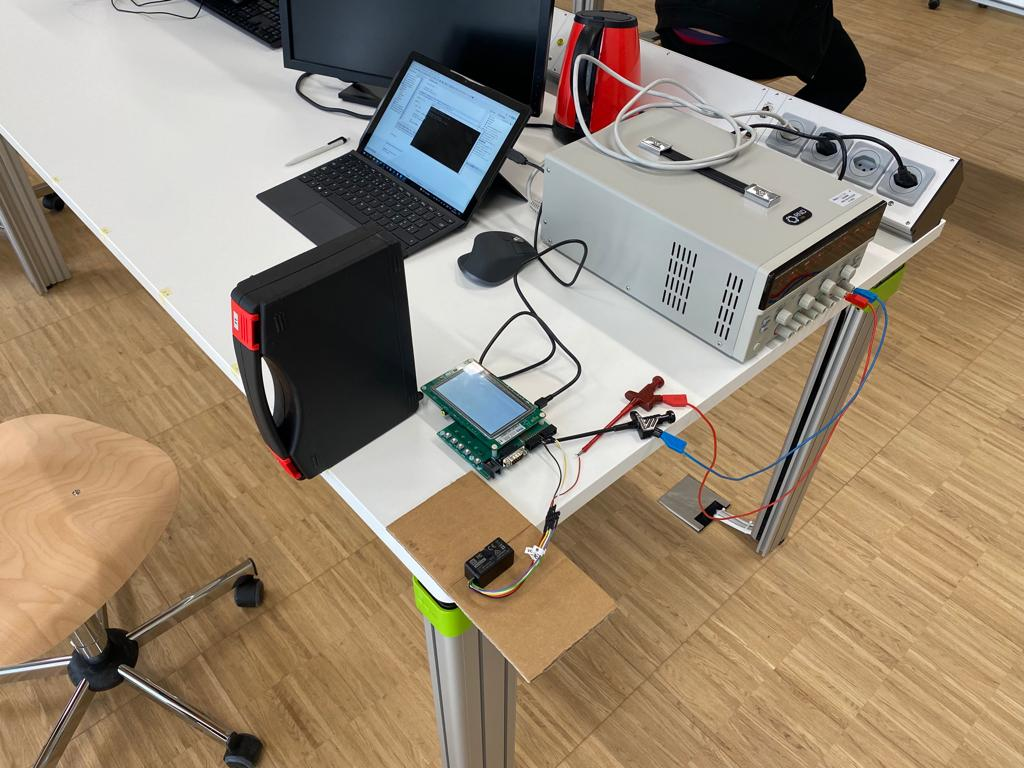
\includegraphics[width=0.5\textwidth]{Images/LiDAR/RealDistanceMes.jpeg}
    \caption{Mesure de distance comparée à la distance réelle}
    \label{fig:RealDistanceMeasures}
\end{figure}

La mesure finale de distance est une moyenne de 10 mesures. Cela permet notamment d'éliminer partiellement
l'erreur due à la résolution finie du capteur.\\
Le test a été réalisé en intérieur, en l'absence total d'élément perturbateur, notamment de rayons 
infrarouges, à température ambiante (25°C).

\subsubsection{Résultats du test}

\begin{figure}[H]
    \centering
    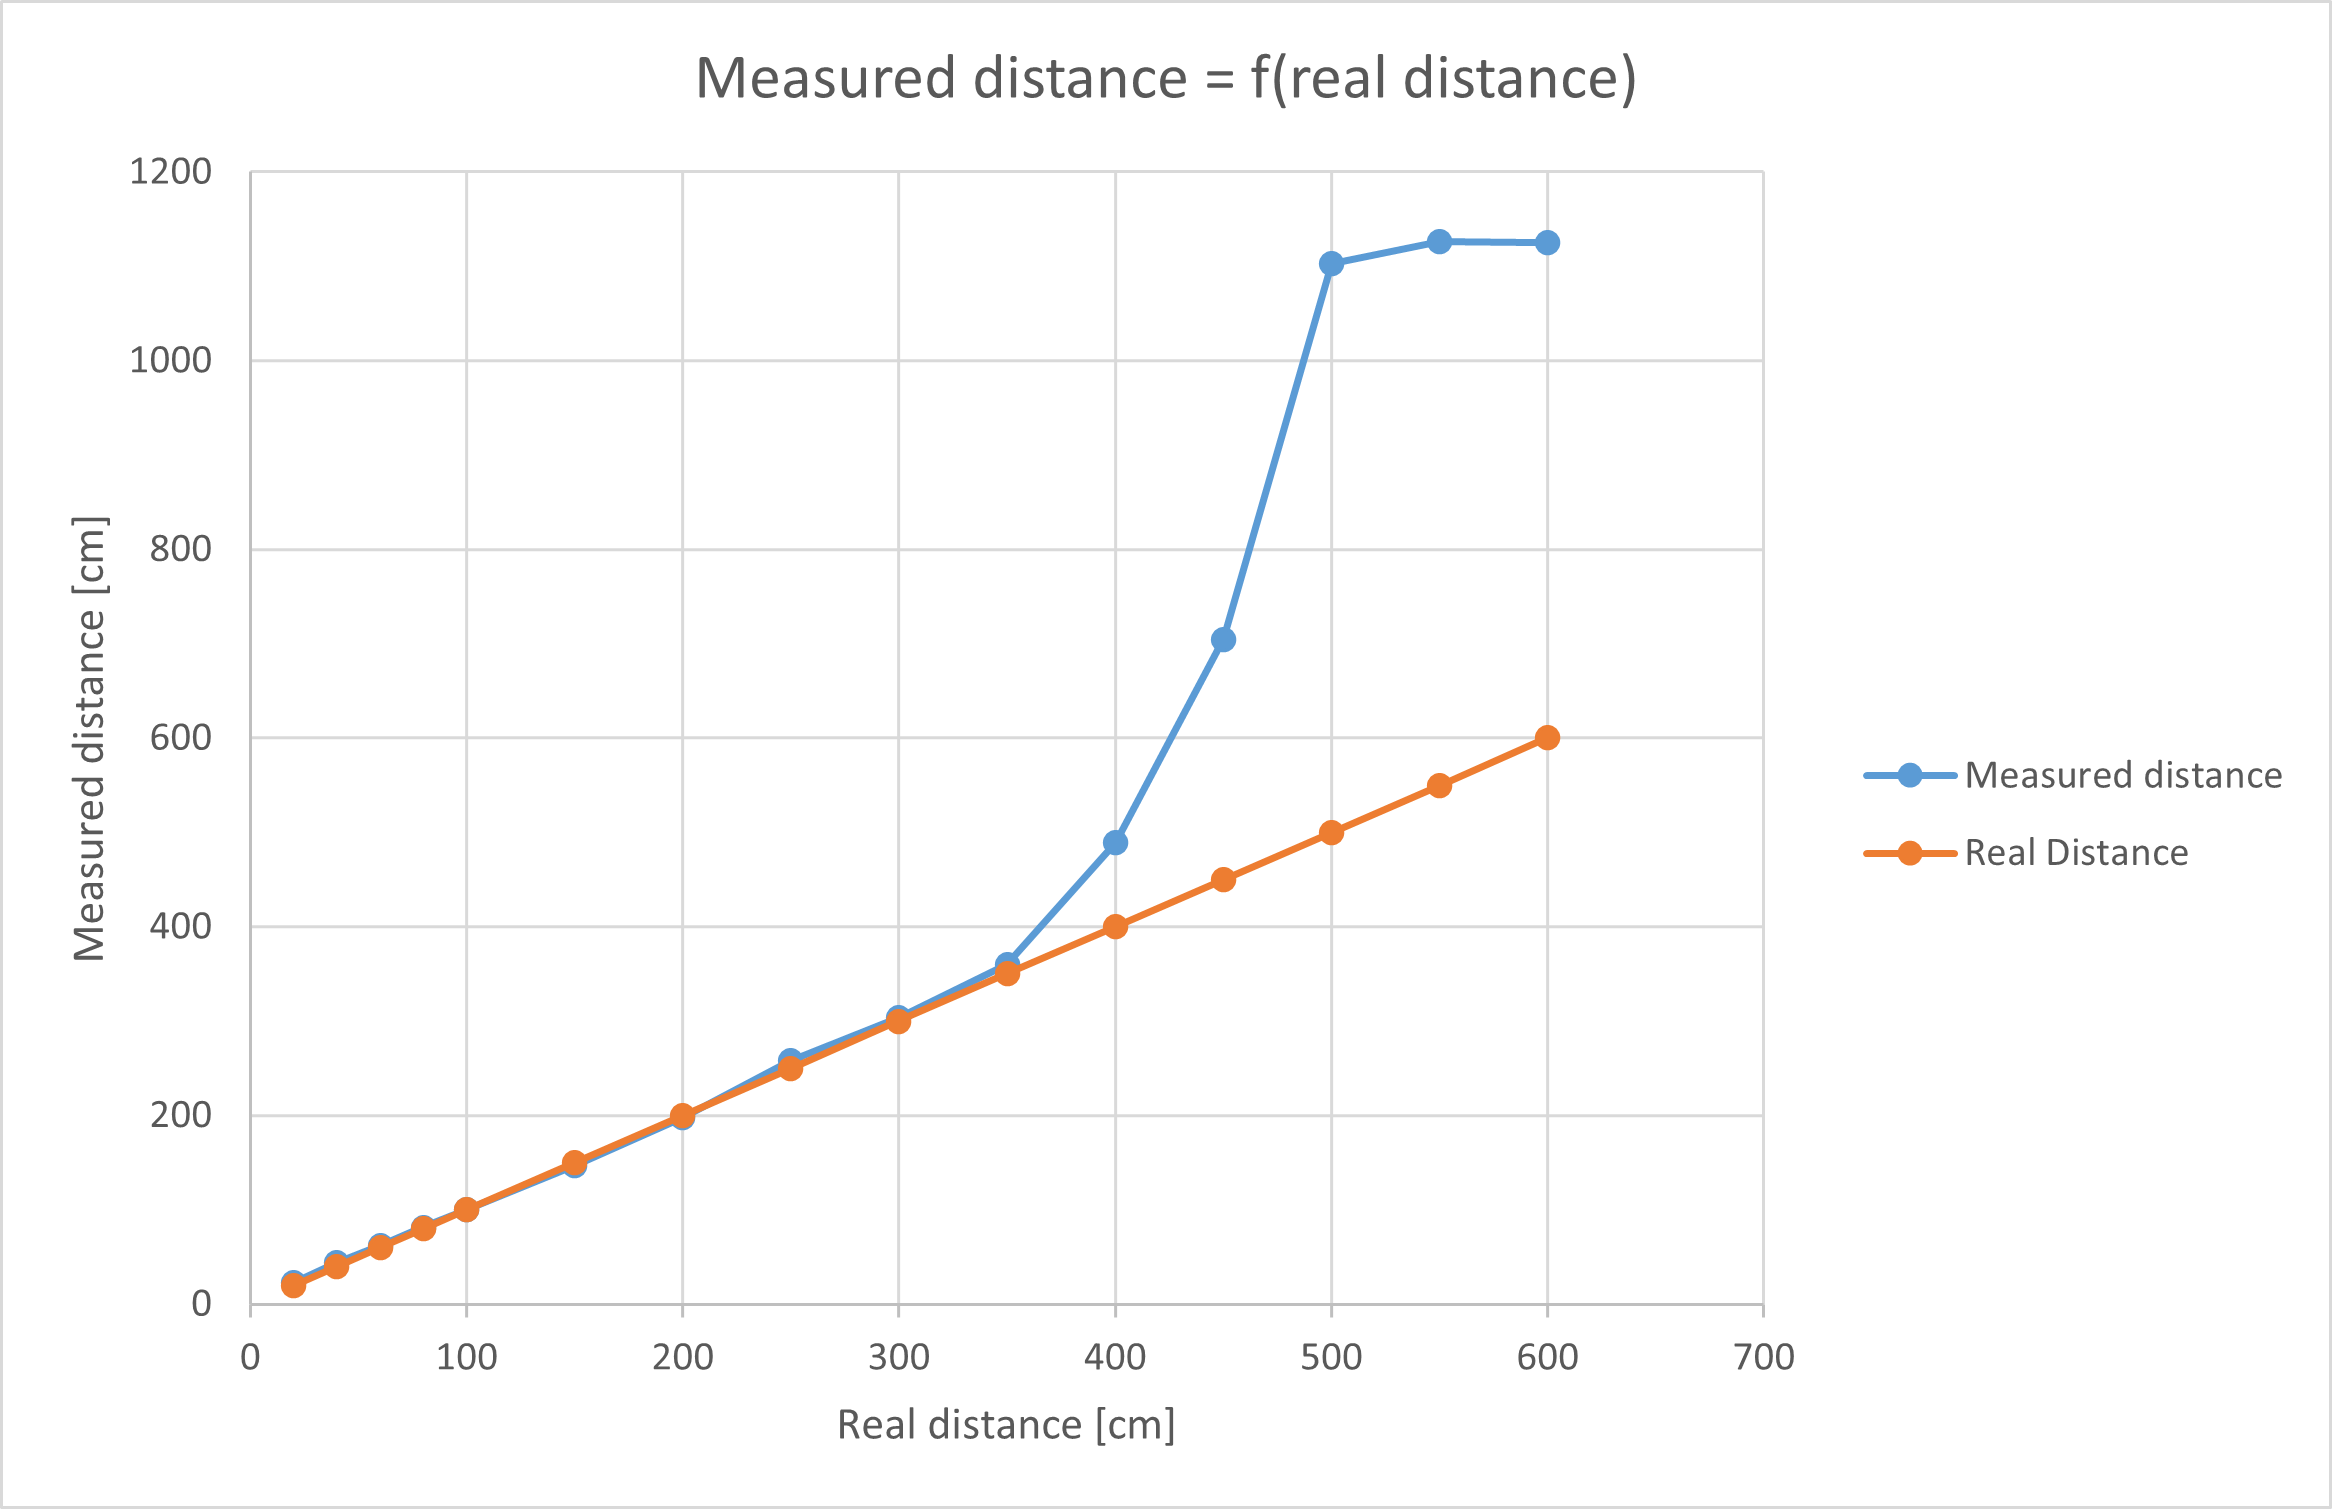
\includegraphics[width=0.8\textwidth]{Images/LiDAR/LiDARRealDistanceGraph_MesDist.png}
    \caption{Distance mesurée en fonction de la distance réelle}
    \label{fig:RealDistanceMesGraph}
\end{figure}

\begin{figure}[H]
    \centering
    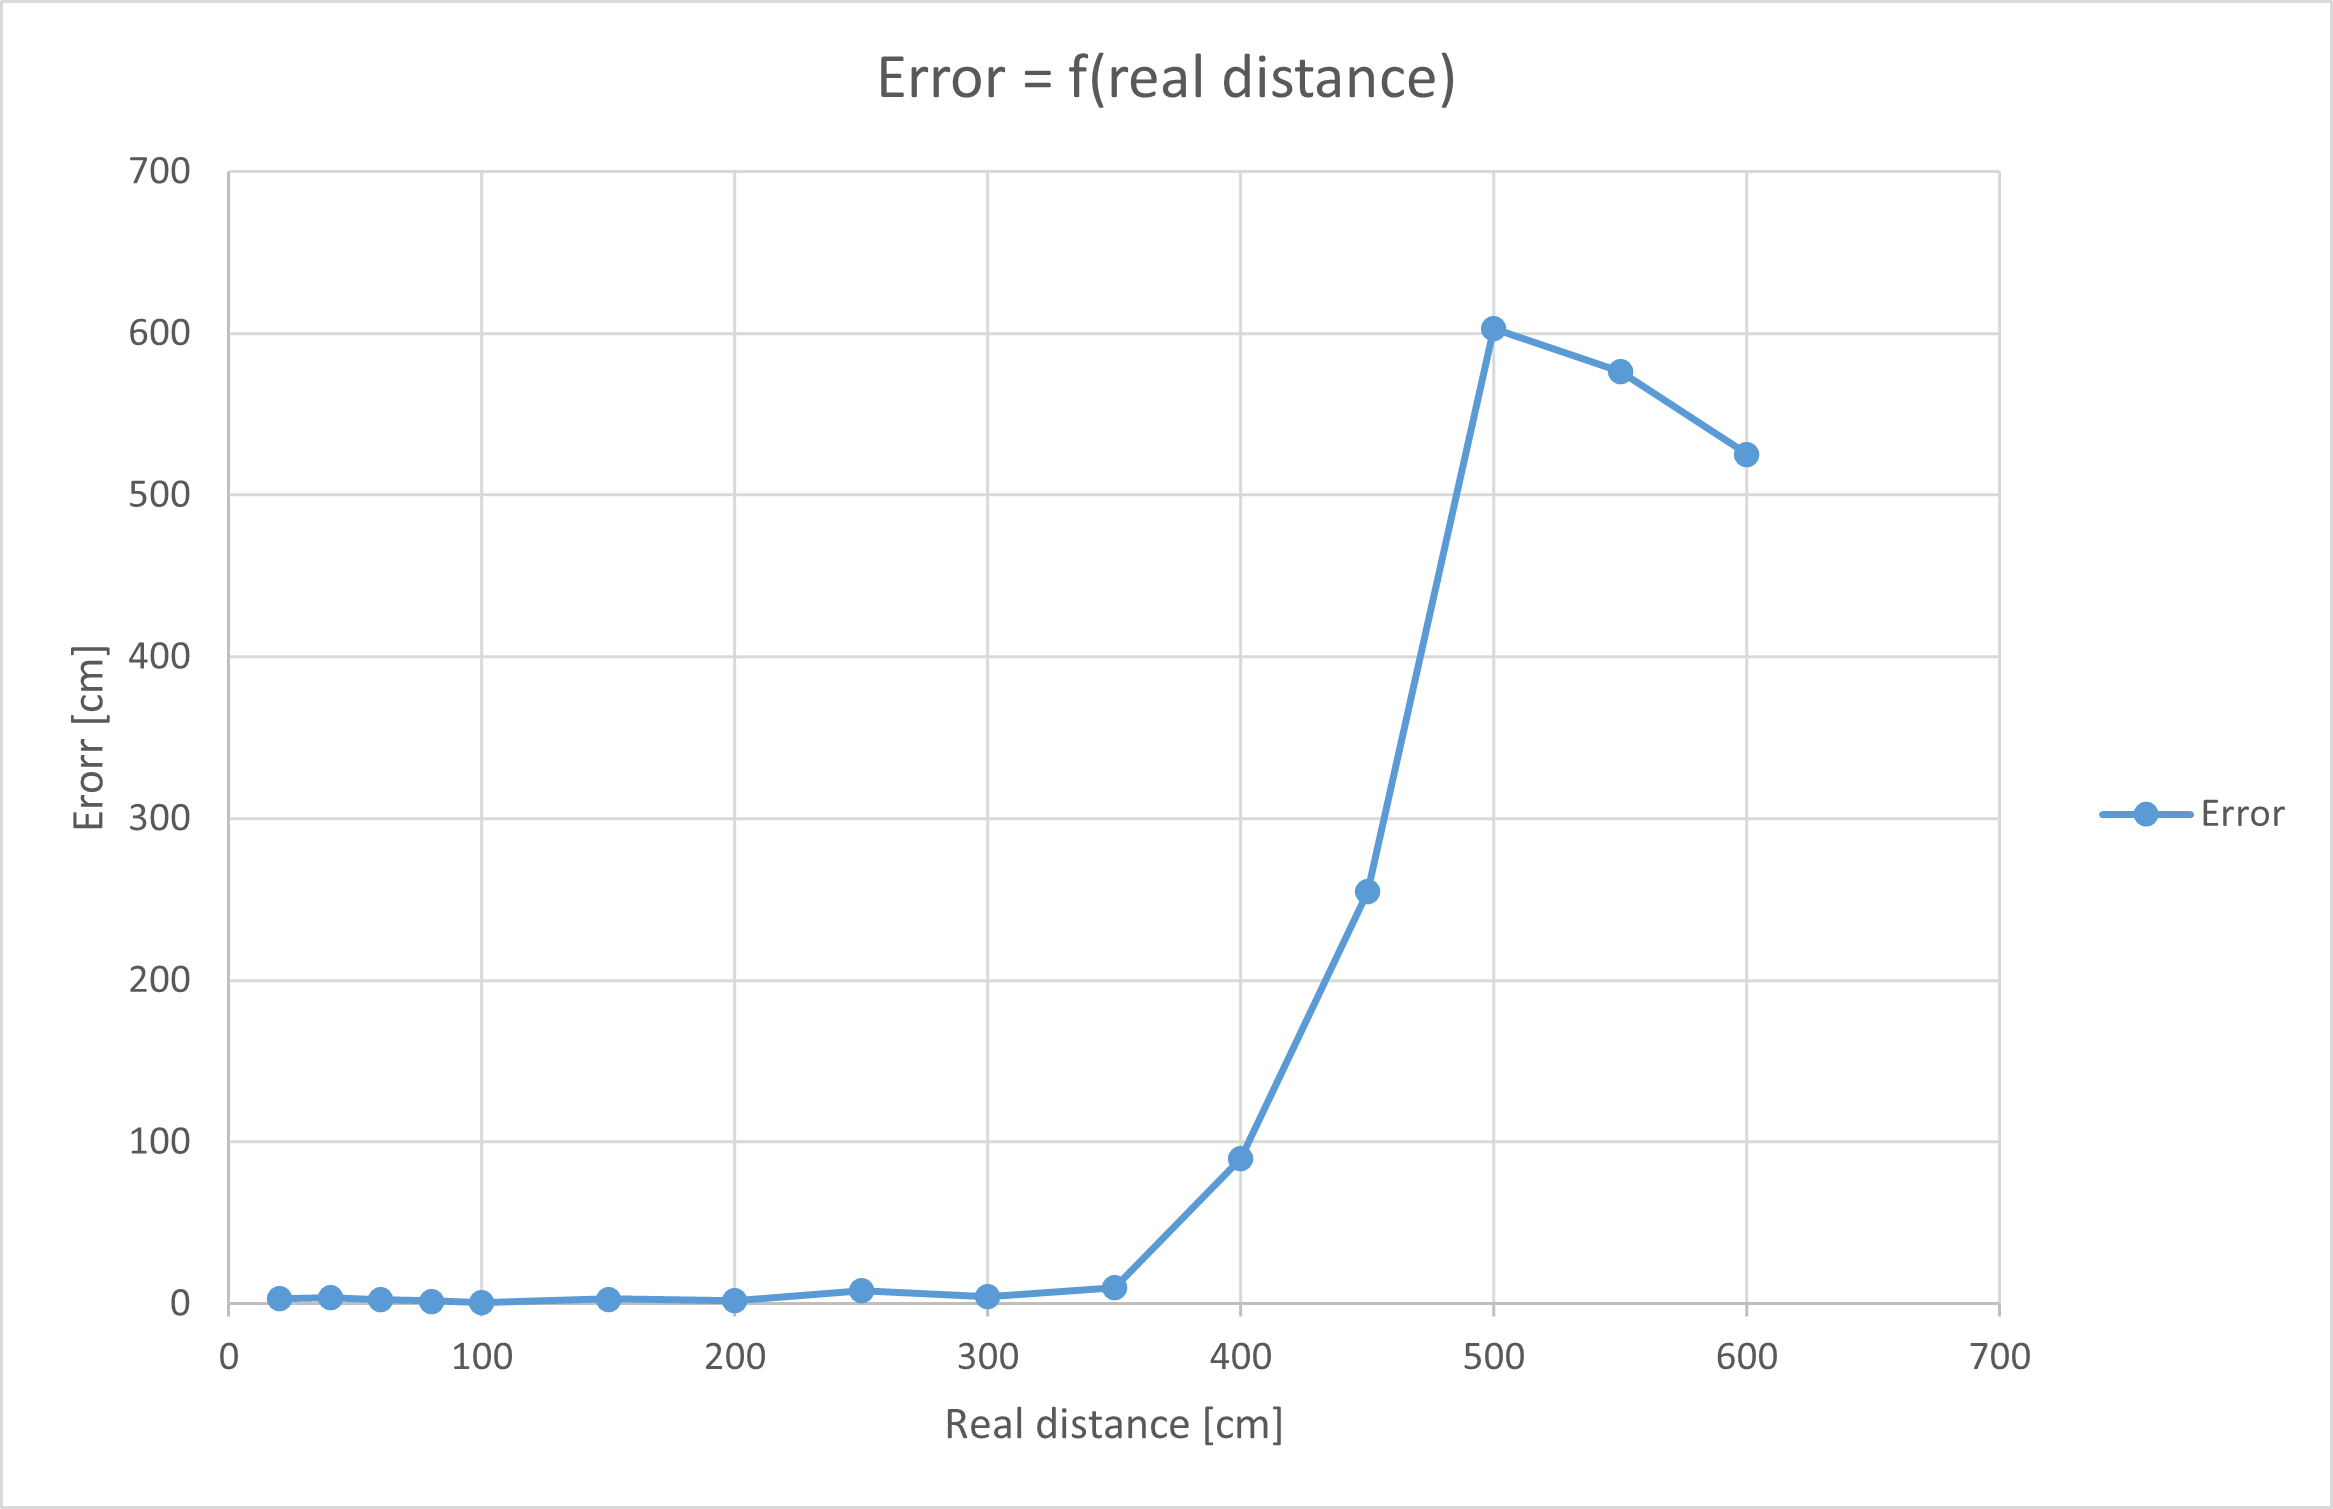
\includegraphics[width=0.8\textwidth]{Images/LiDAR/LiDARRealDistanceGraph_MesDistError.png}
    \caption{Erreur de la distance mesurée par rapport à la distance réelle}
    \label{fig:RealDistanceMesGraphError}
\end{figure}

Nous avons jugé important de zoomer sur la plage utile entre 0 et 3m afin de visualiser les graphes 
de manière plus claire.

\begin{figure}[H]
    \centering
    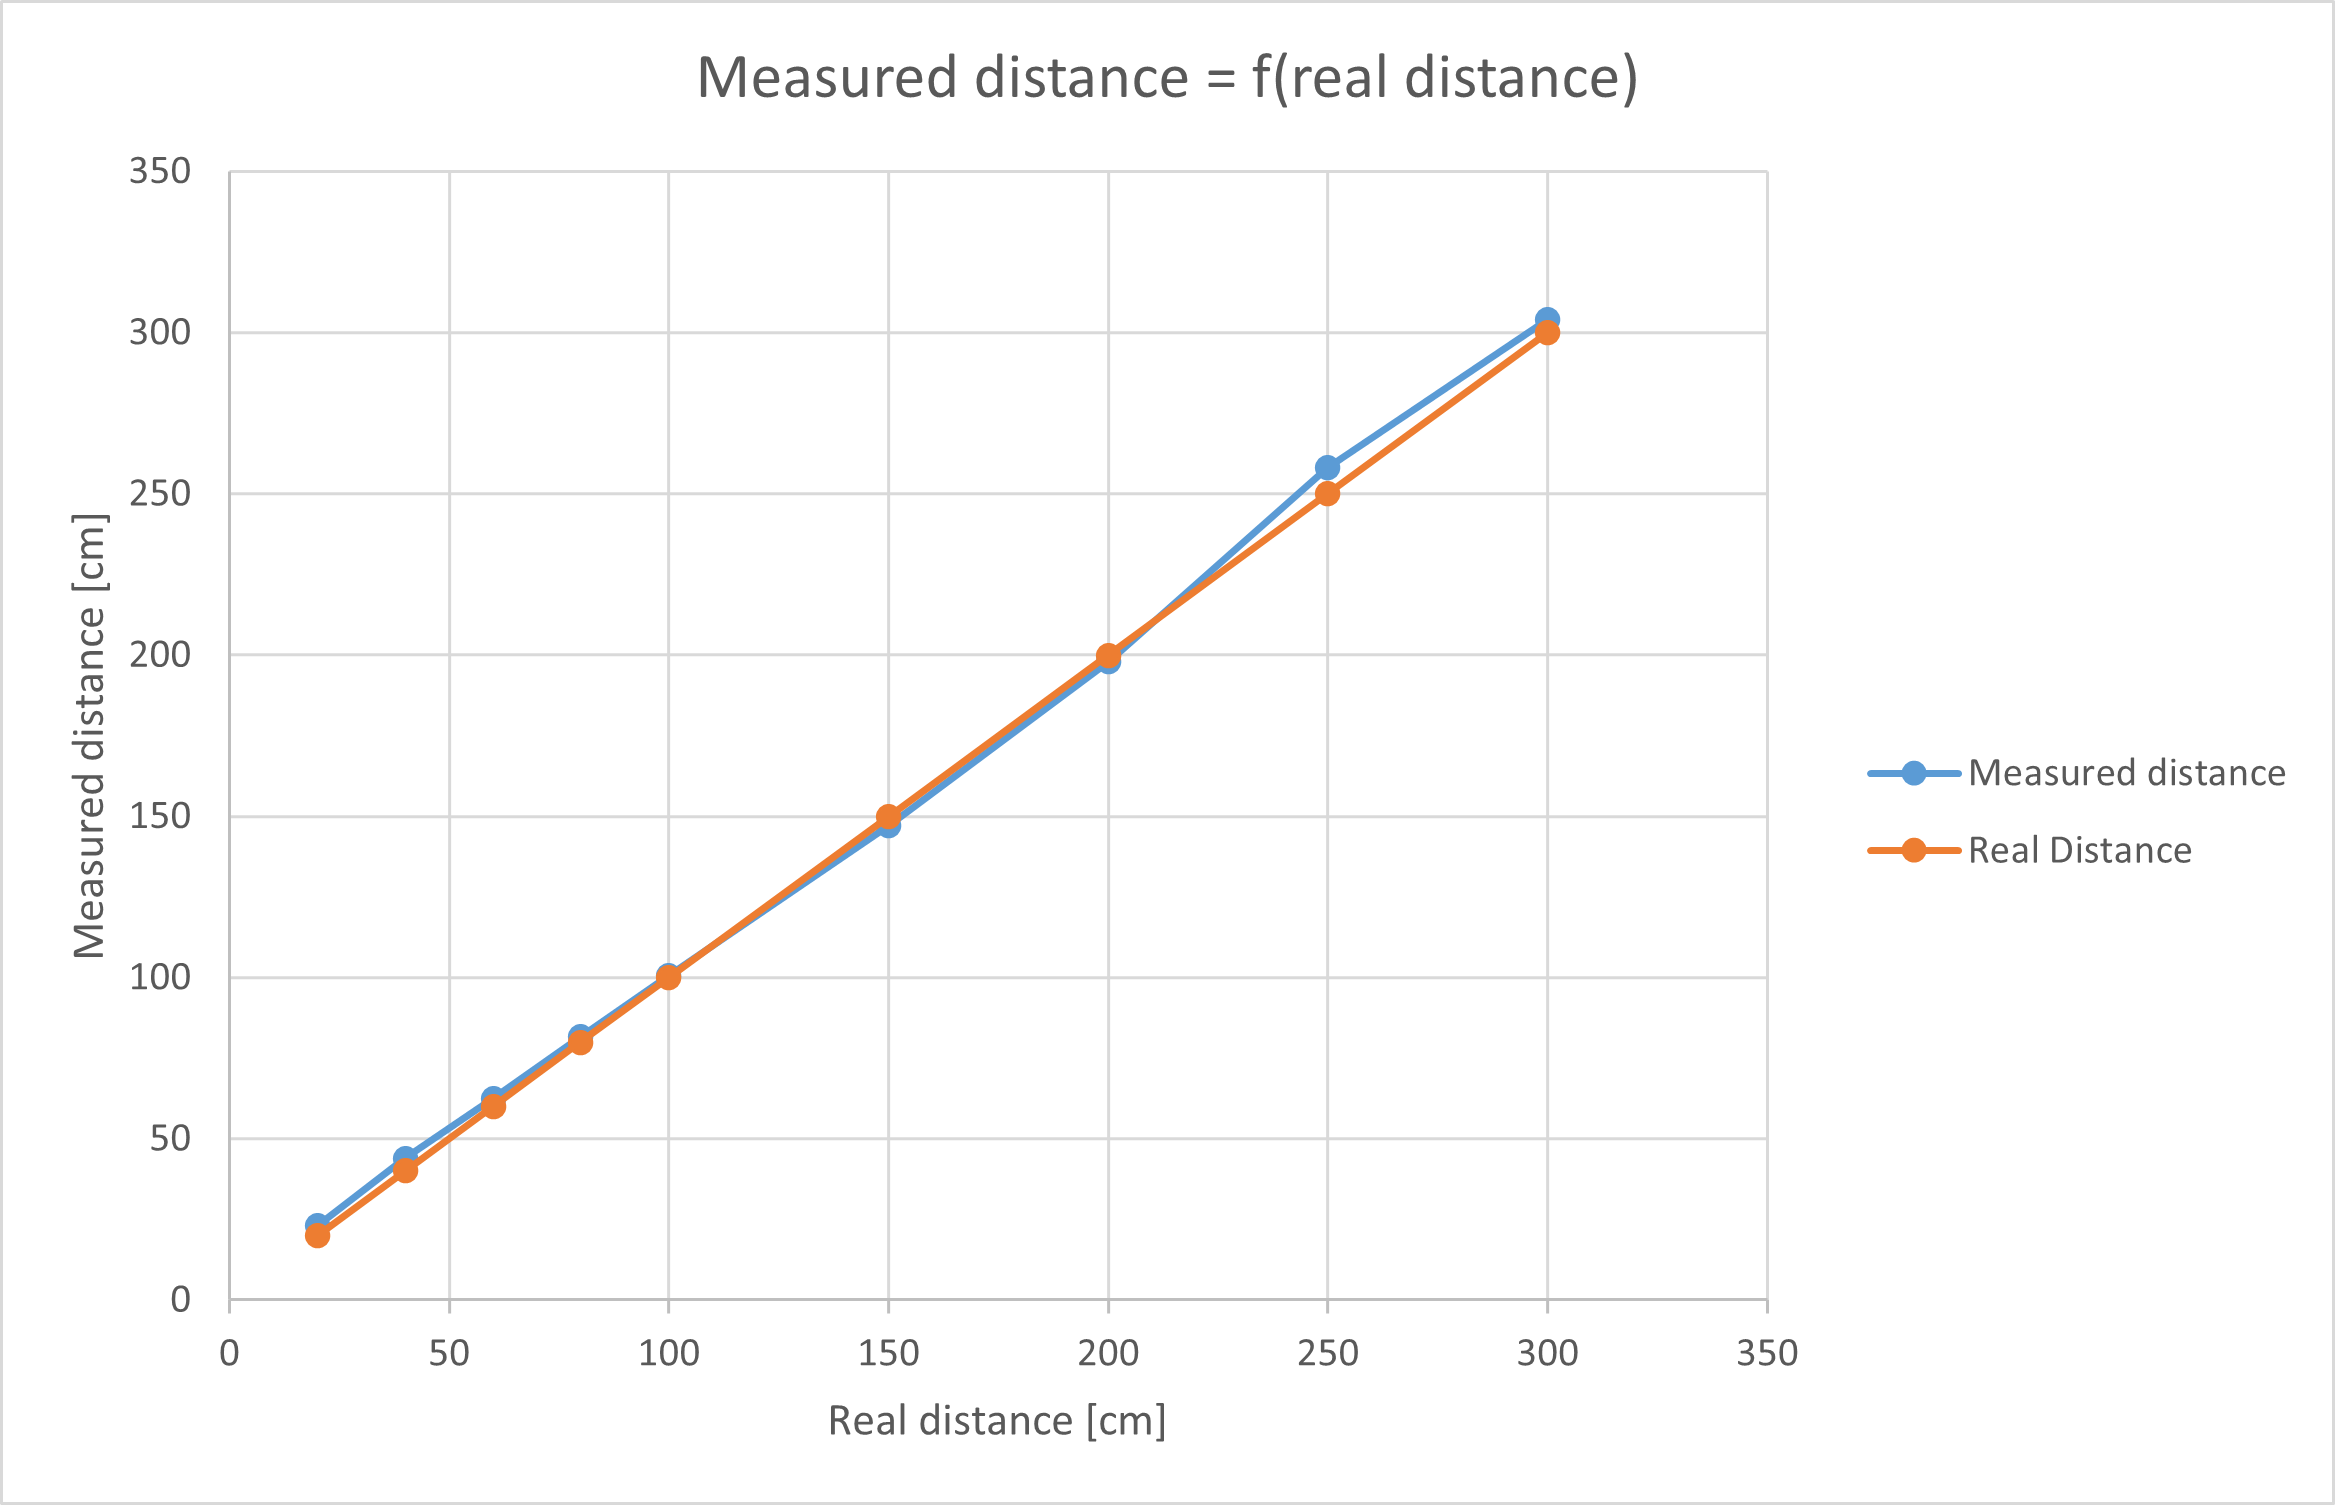
\includegraphics[width=0.8\textwidth]{Images/LiDAR/LiDARRealDistanceGraph_MesDist_Zoom.png}
    \caption{Distance mesurée en fonction de la distance réelle dans la plage utile}
    \label{fig:RealDistanceMesGraphZoom}
\end{figure}

\begin{figure}[H]
    \centering
    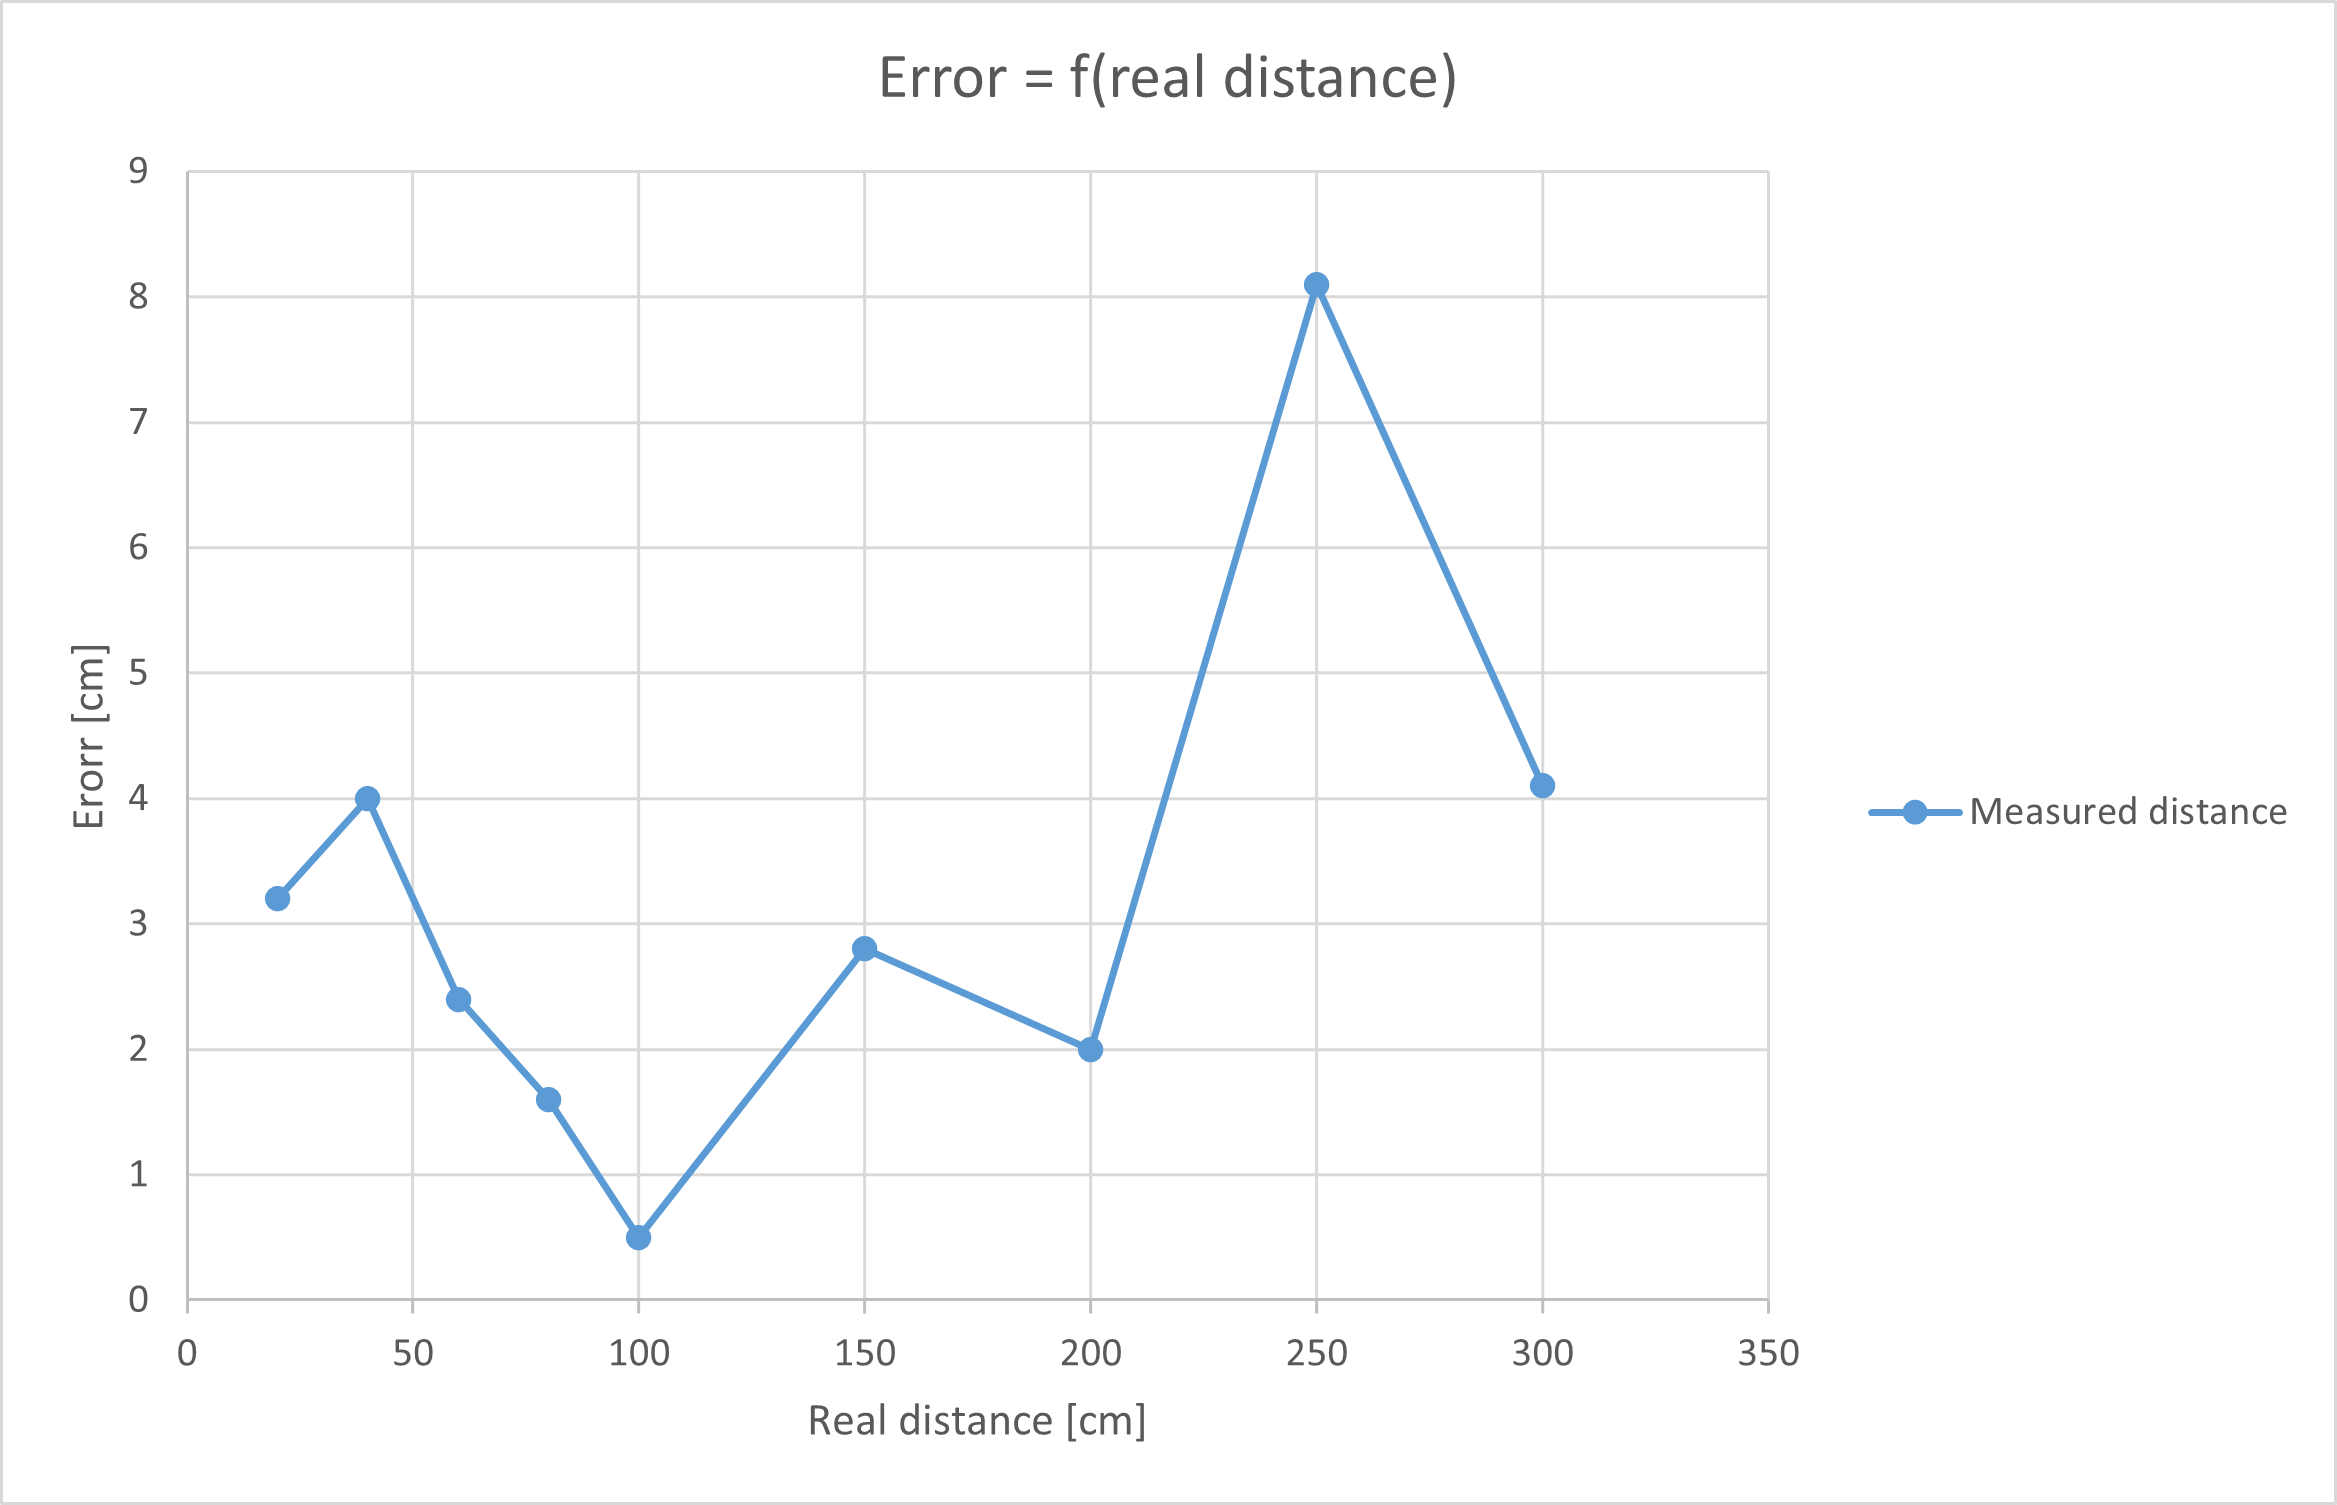
\includegraphics[width=0.8\textwidth]{Images/LiDAR/LiDARRealDistanceGraph_MesDistError_Zoom.png}
    \caption{Erreur de la distance mesurée par rapport à la distance réelle dans la plage utile}
    \label{fig:RealDistanceMesGraphErrorZoom}
\end{figure}

\subsubsection{Conclusion préliminaire}

On constate très facilement sur la figure \ref{fig:RealDistanceMesGraph} que le capteur est perdu au delà
de 3.5m, soit bien moins qu'annoncé par le fabricant. La figure \ref{fig:RealDistanceMesGraphError} nous 
montre une erreur absurde de plus de 5 mètres. On conclut donc que ce capteur ne pourra pas être utilisé
pour des distances de plus de 3.5m.\\
Comme cette grande erreur aplatit totalement les mesures sous 3.5m, nous avons jugé utile d'effectuer un
zoom sur cette plage utile. On constate alors que la distance mesurée par le LiDAR reflète avec plus ou
moins de précision la distance réelle, comme le montre la figure \ref{fig:RealDistanceMesGraphZoom}.
Lorsqu'on trace l'erreur en fonction de la distance réelle, on remarque une erreur généralement bien plus
élevée qu'annoncé (figure \ref{fig:RealDistanceMesGraphErrorZoom}), soit \textpm 1cm pour des distances de 
moins de 2m et \textpm 2cm entre 2 et 4m. Cependant, il faut se rappeler que ce graphe montre uniquement 
l'erreur à la distance réelle, et non l'erreur de répétabilité. Or, comme ces mesures sont un condensé 
de plusieurs séquences espacées dans le temps, on remarque que l'erreur est constante, qui donc peut 
être compensée. De plus, dans le projet, on ne travaille qu'avec des offsets, ce qui limite d'autant 
plus les effets de cette erreur.\par

On peut finalement conclure que ce test est réussi. En effet, malgré une erreur non-négligeable de mesure,
le capteur a une répétabilité constante. Nous pouvons donc passer au test suivant.

\subsection{Mesures de distance dans un environnement perturbé}
\label{fig:MesNoise}

Maintenant que nous savons que le capteur a une répétabilité acceptable, nous cherchons à déterminer comment 
le LiDAR réagit dans un environnement perturbé. Ainsi, un banc de test a été construit afin de projeter 
des confettis devant le capteur lorsqu'il mesure. Les détails de sa construction sont expliqués dans la
section correspondante. Le but final est de générer du bruit de mesure afin de représenter au mieux une
situation réelle, par exemple en pleine tempête de neige. Nous pourrons ainsi développer une méthode
de mesure qui permet en tout temps de mesurer une hauteur de neige.

\subsubsection{Méthode}

Afin de vérifier ce test, le capteur ainsi que la plaque de développement ont été montés sur un trépied
à environ 1.5m au-dessus du sol, avec un angle de 60° par rapport à la verticale. Le LiDAR pointe le sol,
nettoyé au préalable et donc sans confetti. 100 mesures de distance sont réalisées à chaque série afin
d'avoir assez d'échantillons pour quantifier le bruit généré.\\
Sur l'appui du bouton utilisateur de la carte, le programme lance une série de 100 mesures en direction
du sol. Cela nous permet dans un premier temps d'avoir une distance de référence à comparer, sans aucune
perturbation. \\
Ensuite, quatre autres séries de mesures sont effectuées, avec quatre niveaux arbitraires de perturbation
différents, générés manuellement par les opérateurs, comme le montre la figure \ref{fig:ErrorMesSetup}.

\begin{figure}[H]
    \centering
    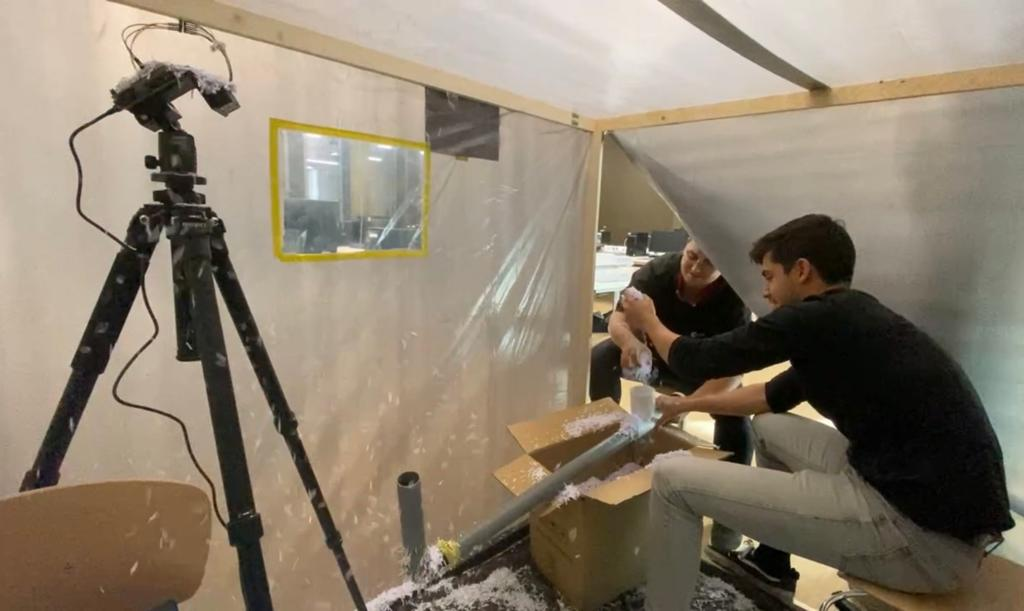
\includegraphics[width=0.75\textwidth]{Images/LiDAR/ErrorMesSetup.jpeg}
    \caption{Mise en place du test de perturbation}
    \label{fig:ErrorMesSetup}
\end{figure}

\subsubsection{Résultats du test}

\begin{figure}[H]
    \centering
    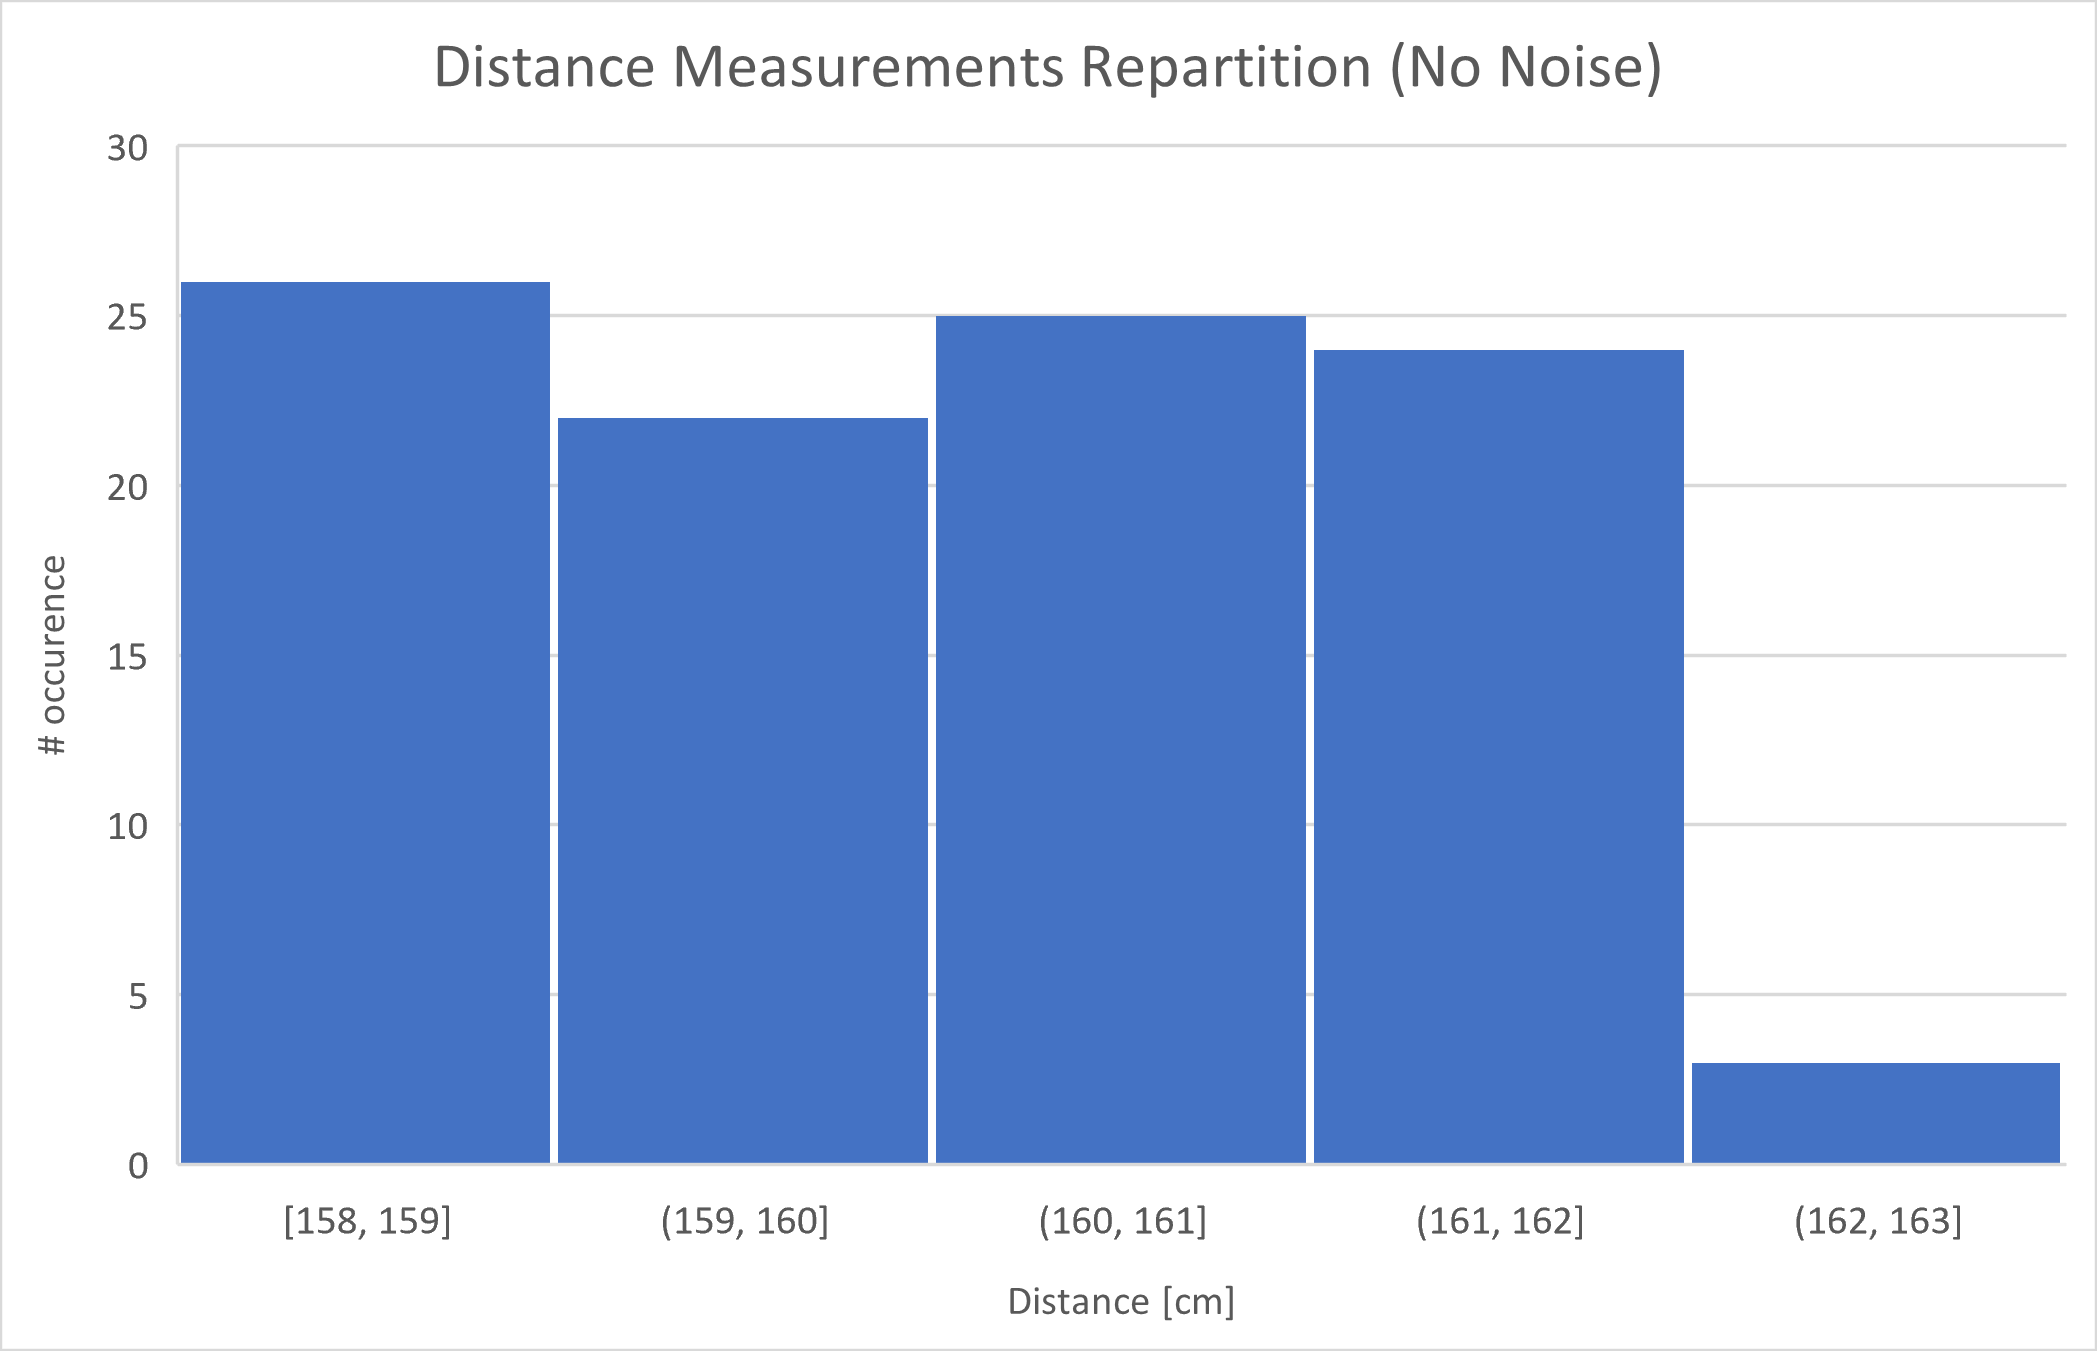
\includegraphics[width=0.8\textwidth]{Images/LiDAR/LiDAR_ErrorMes_NoNoise.png}
    \caption{Histogramme de la mesure de référence}
    \label{fig:ErrorMesRefDist}
\end{figure}

\begin{figure}[H]
    \centering
    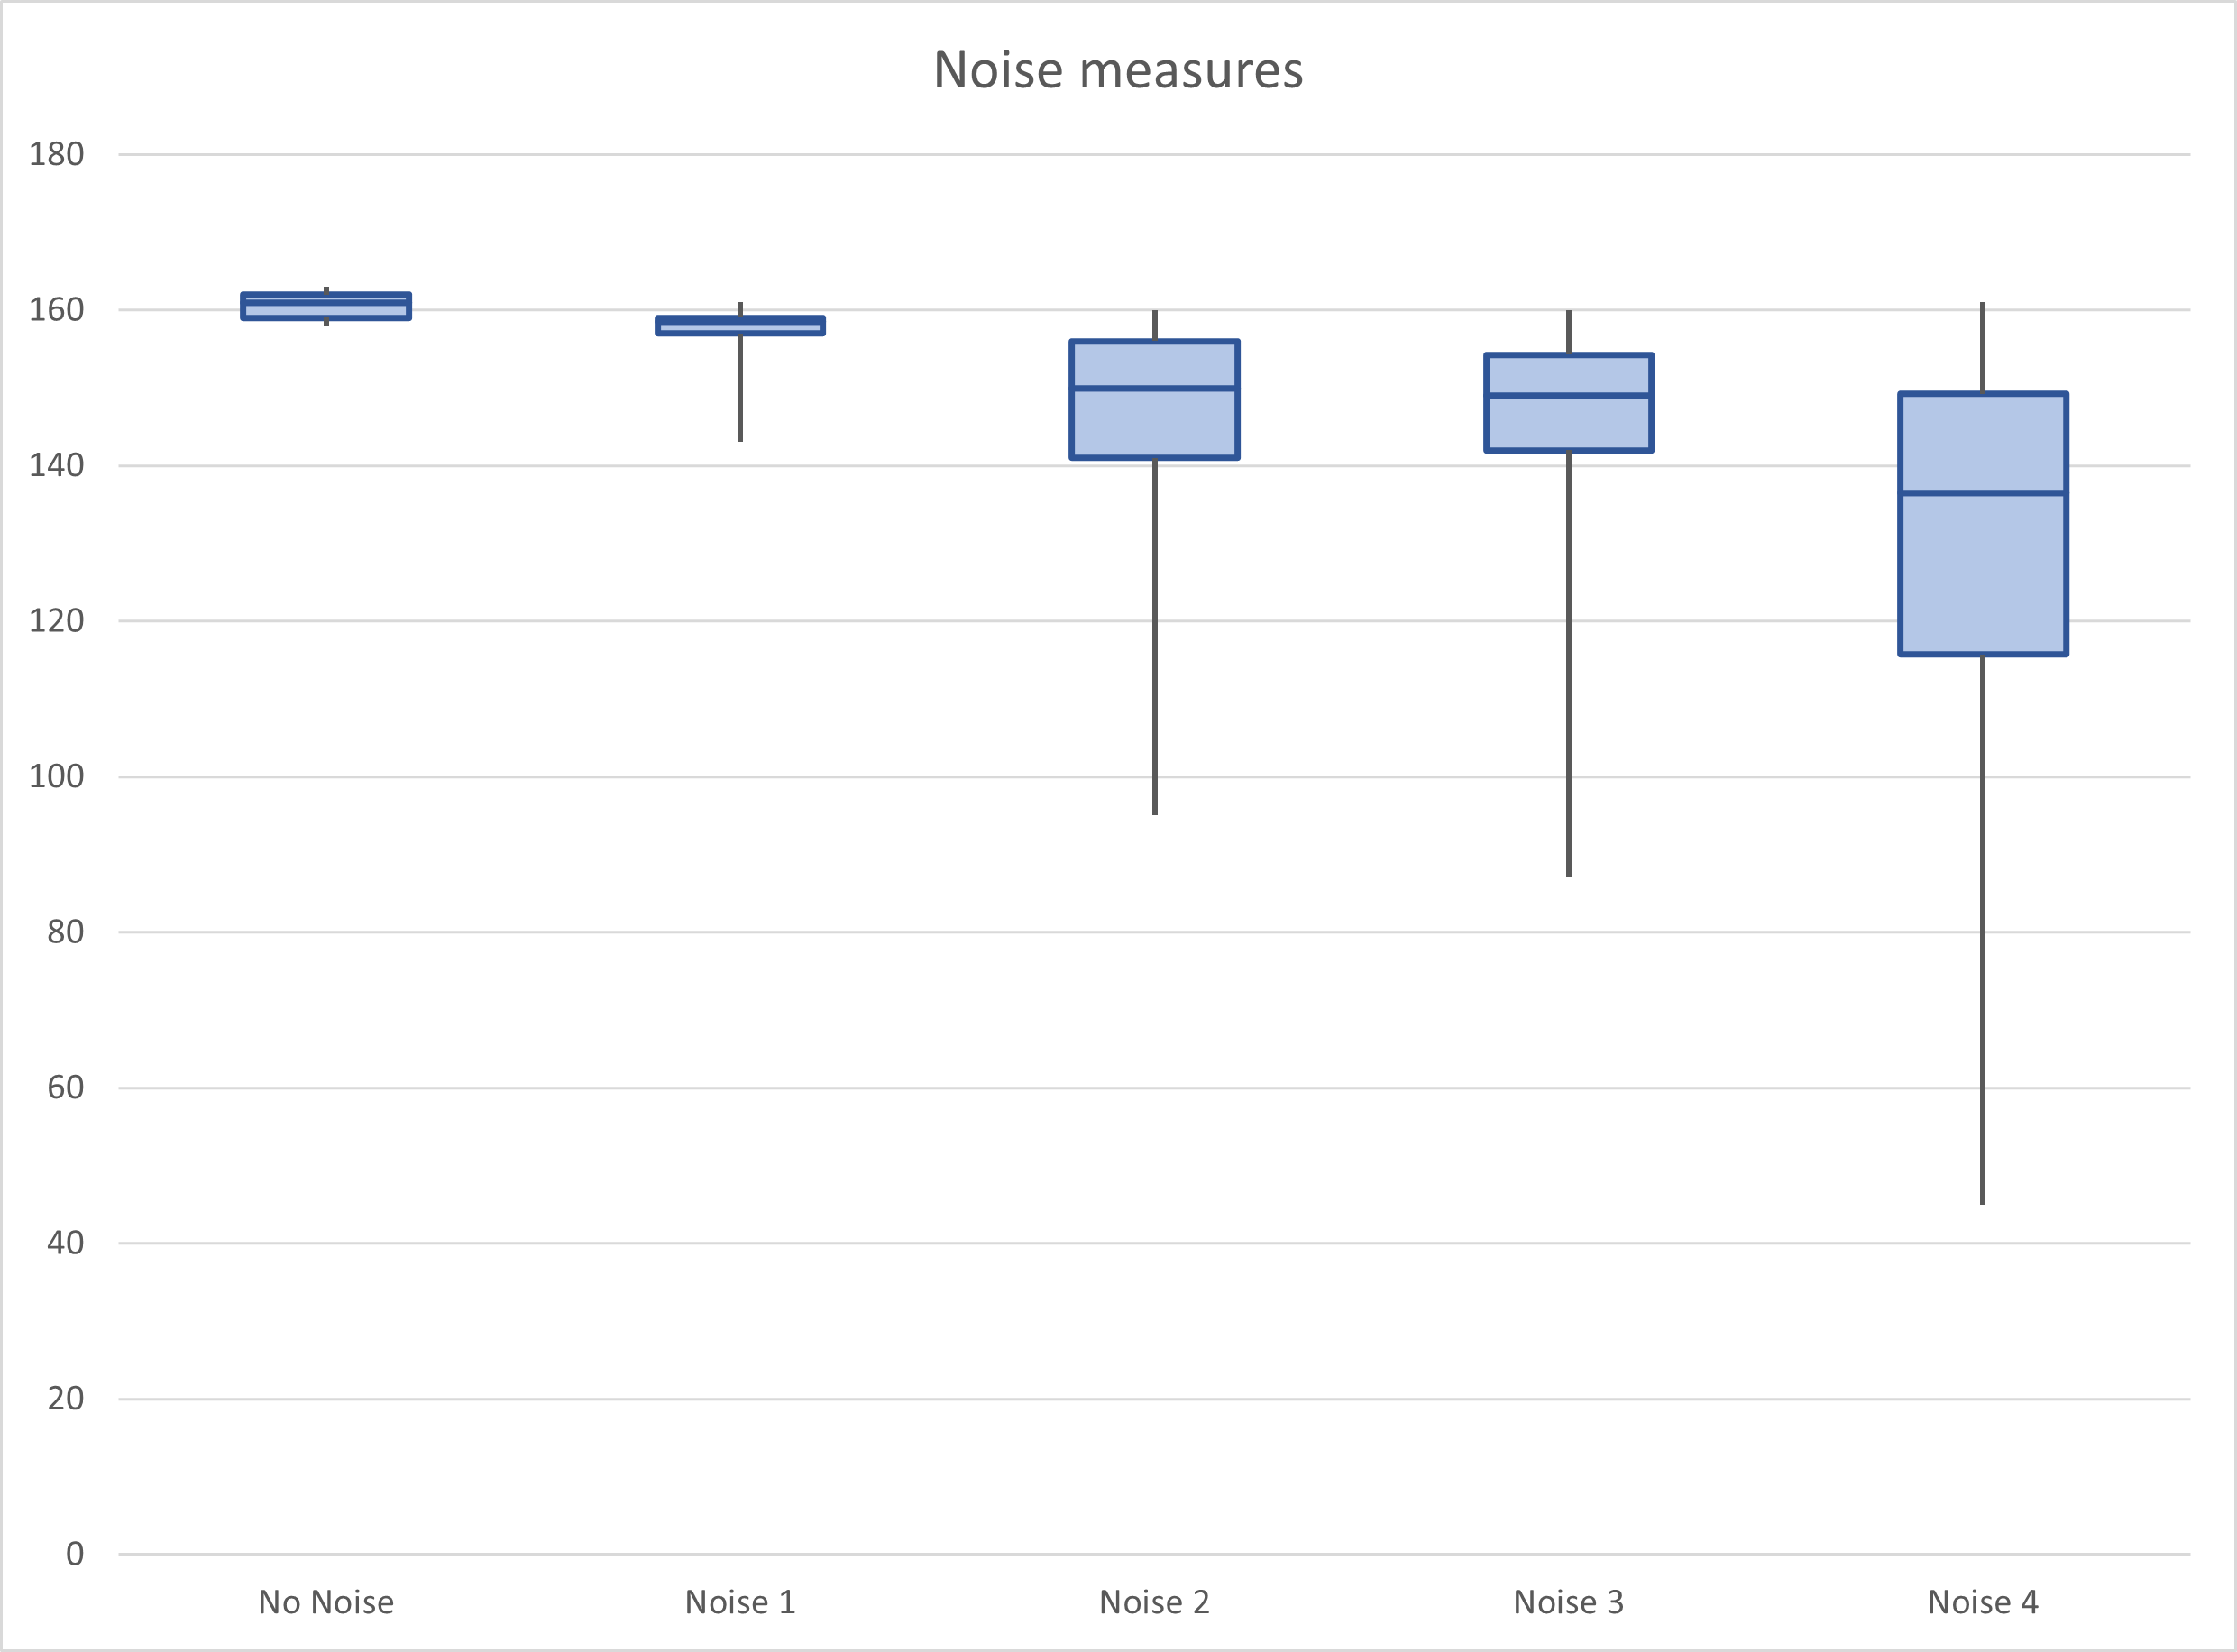
\includegraphics[width=0.8\textwidth]{Images/LiDAR/LiDAR_ErrorMes_Moustache.png}
    \caption{Comparaison des 5 mesures effectuées}
    \label{fig:ErrorMesMoustache}
\end{figure}

Les 5 mesures ont été regroupées en un seul graphe de type "Boîte à moustaches" afin de pouvoir
comparer avec plus d'aisance les mesures entre-elles. De gauche à droite, on retrouve une augmentation
graduelle du bruit généré par les opérateurs.

\begin{table}[H]
    \centering
    \begin{tabular}{|c|c|c|c|c|c|}
        \hline
        & No Noise & Noise 1 & Noise 2 & Noise 3 & Noise 4 \\
        \hline\hline
        Mean & 160.52 & 157.77 & 145.44 & 145.06 & 127.78 \\
        \hline
        Median & 161 & 158.8 & 150 & 149 & 136.5 \\
        \hline
        Max & 163 & 161 & 160 & 160 & 161 \\
        \hline
        
    \end{tabular}
    \caption{Différentes méthodes de calcul de distance (en cm)}
    \label{table:ComputingMethods}
\end{table}

Afin d'avoir la méthode la plus représentative possible de la distance au sol, trois solutions 
ont été envisagées. À partir de la série de mesures, nous avons calculé la moyenne, la médiane
ainsi que le maximum afin de déterminer laquelle de ces valeurs représente le plus la réalité.\\
//ANNEXE A : HISTOGRAMME DE CHACUNE DES MESURES

\subsubsection{Conclusion préliminaire} 

Premièrement, la figure \ref{fig:ErrorMesRefDist} montre l'histogramme des 100 mesures de référence au sol.
Elles s'avèrent plutôt rassurantes car on remarque que la répétabilité des mesures est respectée, avec
une précision typique de \textpm 2cm. La plupart des mesures sont réparties uniformément autour de 160cm.\par
On distingue ensuite sur la figure \ref{fig:ErrorMesMoustache} que le bruit de mesure a bel et bien augmenté
au fil des séries, représenté par la longueur des barres d'erreur. Comme l'indique le principe des boîtes
à moustache, le trait central du rectangle représente la médiane des valeurs, alors que les deux autres
sont le premier et troisième quartiles. Ainsi, les valeurs médianes des séries s'éloignent de plus en 
plus de la distance au sol (de référence).\par
Le but final de la figure \ref{fig:ErrorMesMoustache} est d'aider à déterminer quelle est la méthode
de mesure la plus efficace pour calculer des distances dans un environnement perturbé. On remarque
ainsi d'ores et déjà que la médiane n'est pas un outil fiable, puisque sa valeur d'éloigne de plus en
plus de la référence au fil des séries. Cependant, on voit facilement que les valeurs maximales de chaque
boîte s'approche très fortement de la distance de référence.\\
La table \ref{table:ComputingMethods} nous aide à y voir plus clair en ce qui concerne l'efficacité de ces
trois méthodes. Pour rappel, selon la mesure de référence, la distance au sol à mesurer est de 160cm.

\begin{description}
    \item[Moyenne] \hfill \\ 
    La moyenne représente la meilleure méthode dans le cas d'une mesure sans aucune 
    perturbation. Cependant, on voit que cette méthode devient très imprécise lorsque du bruit
    apparaît devant le capteur.
    \item[Médiane] \hfill \\ 
    Malgré le fait que la médiane soit généralement plus proche de la réalité par rapport 
    à la moyenne, elle est encore beaucoup trop éloignée de la vraie distance au sol. L'erreur est à 
    nouveau de plus en plus grande dès que les perturbations augmentent. 
    \item[Maximum] \hfill \\ 
    La méthode du maximum semble donner une valeur très proche de la vraie distance,
    et ce peu importe le niveau de perturbation devant le capteur. Il suffit en effet qu'une valeur
    de la série soit la mesure du sol pour que cette méthode fonctionne. Nous comptons donc sur le fait 
    que, statistiquement, on finisse toujours par faire au moins une mesure de la distance au sol dans 
    la série.
\end{description}

Il semblerait que pour le moment, la méthode du maximum obtienne les résultats les plus prometteurs.
Cependant, nous garderons ces 3 méthodes pour les tests suivants afin de confirmer ou non l'efficacité
des techniques de calcul.

\subsection{Stabilité en température des mesures}

Le capteur, intégré dans un boîtier étanche, sera soumis à des températures qui varient constamment,
de -20°C lors d'une nuit glaciale jusqu'à 30 voire 40°C à l'intérieur du boîtier, en plein soleil.
Il est important de savoir comment les mesures prises par le LiDAR vont être influencées par cette 
variation.\\
À titre d'exemple, imaginons que le système prenne une mesure de distance de référence afin d'être
prêt à mesurer des hauteurs de neige. Le soleil vient de se coucher, mais une température de 15°C
reigne encore dans le boîtier. Plus tard dans la nuit, alors qu'il fait -5°C, il commence à neiger.
Le système de détection se met en marche et commence à mesurer des offsets. Ces derniers seront
peut-être faussés par une différence de 20°C entre la mesure de référence et la mesure actuelle !

\subsubsection{Méthode}

Le LiDAR et la plaque de développement sont fixés sur un trépied et sont placés dans une chambre
climatique (de la marque \emph{Vötsch}, modèle 4010) afin de faire varier la température ambiante.
Comme décrit dans le paragraphe ci-dessus, le système sera soumis à des températures entre -20°C et
40°C. C'est pour cela que le capteur sera soumis à cette même plage de températures, par pas de 5°C.\\
La distance entre le capteur et la paroi opposée de la chambre climatique est de 47cm. Les mesures 
sont récupérées via le port COM qui lie la carte à l'ordinateur. La figure \ref{fig:TempError} montre 
la mise en place du test, avec le capteur à l'intérieur de la chambre.

\begin{figure}[H]
    \centering
    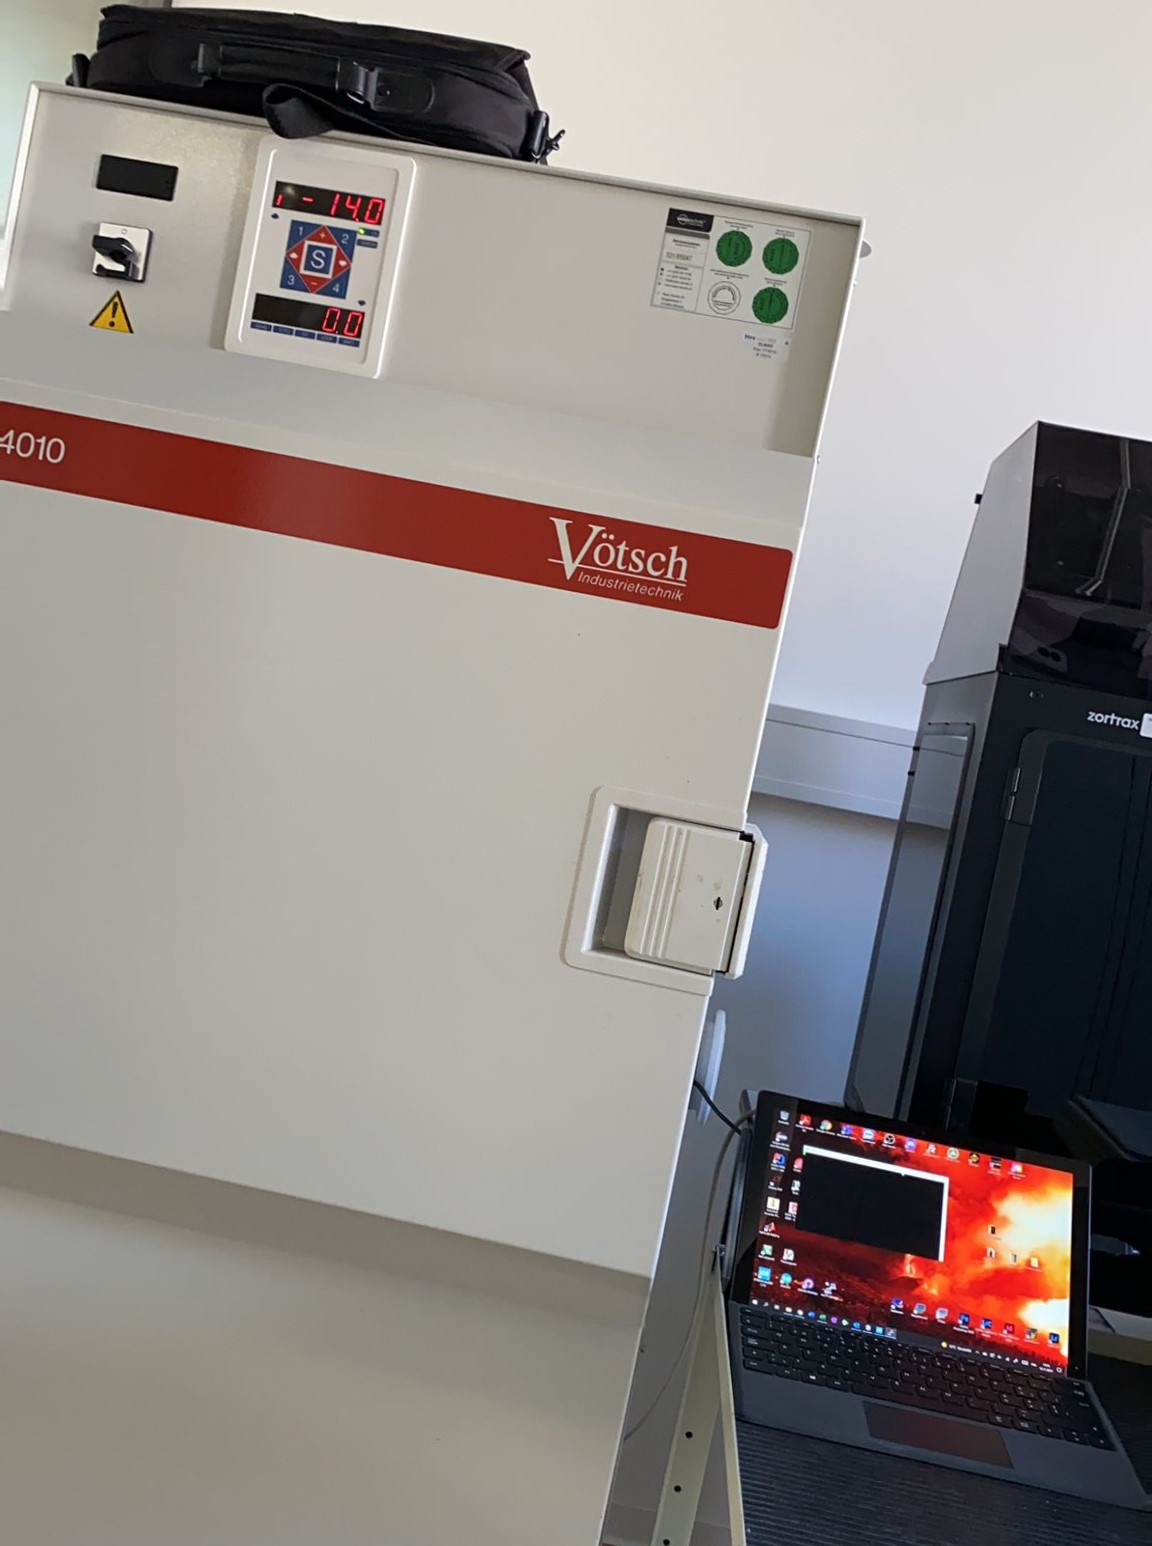
\includegraphics[width=0.5\textwidth]{Images/LiDAR/TempMes.jpeg}
    \caption{Mise en place du test en température}
    \label{fig:TempError}
\end{figure}

\subsubsection{Résultats du test}

\begin{figure}[H]
    \centering
    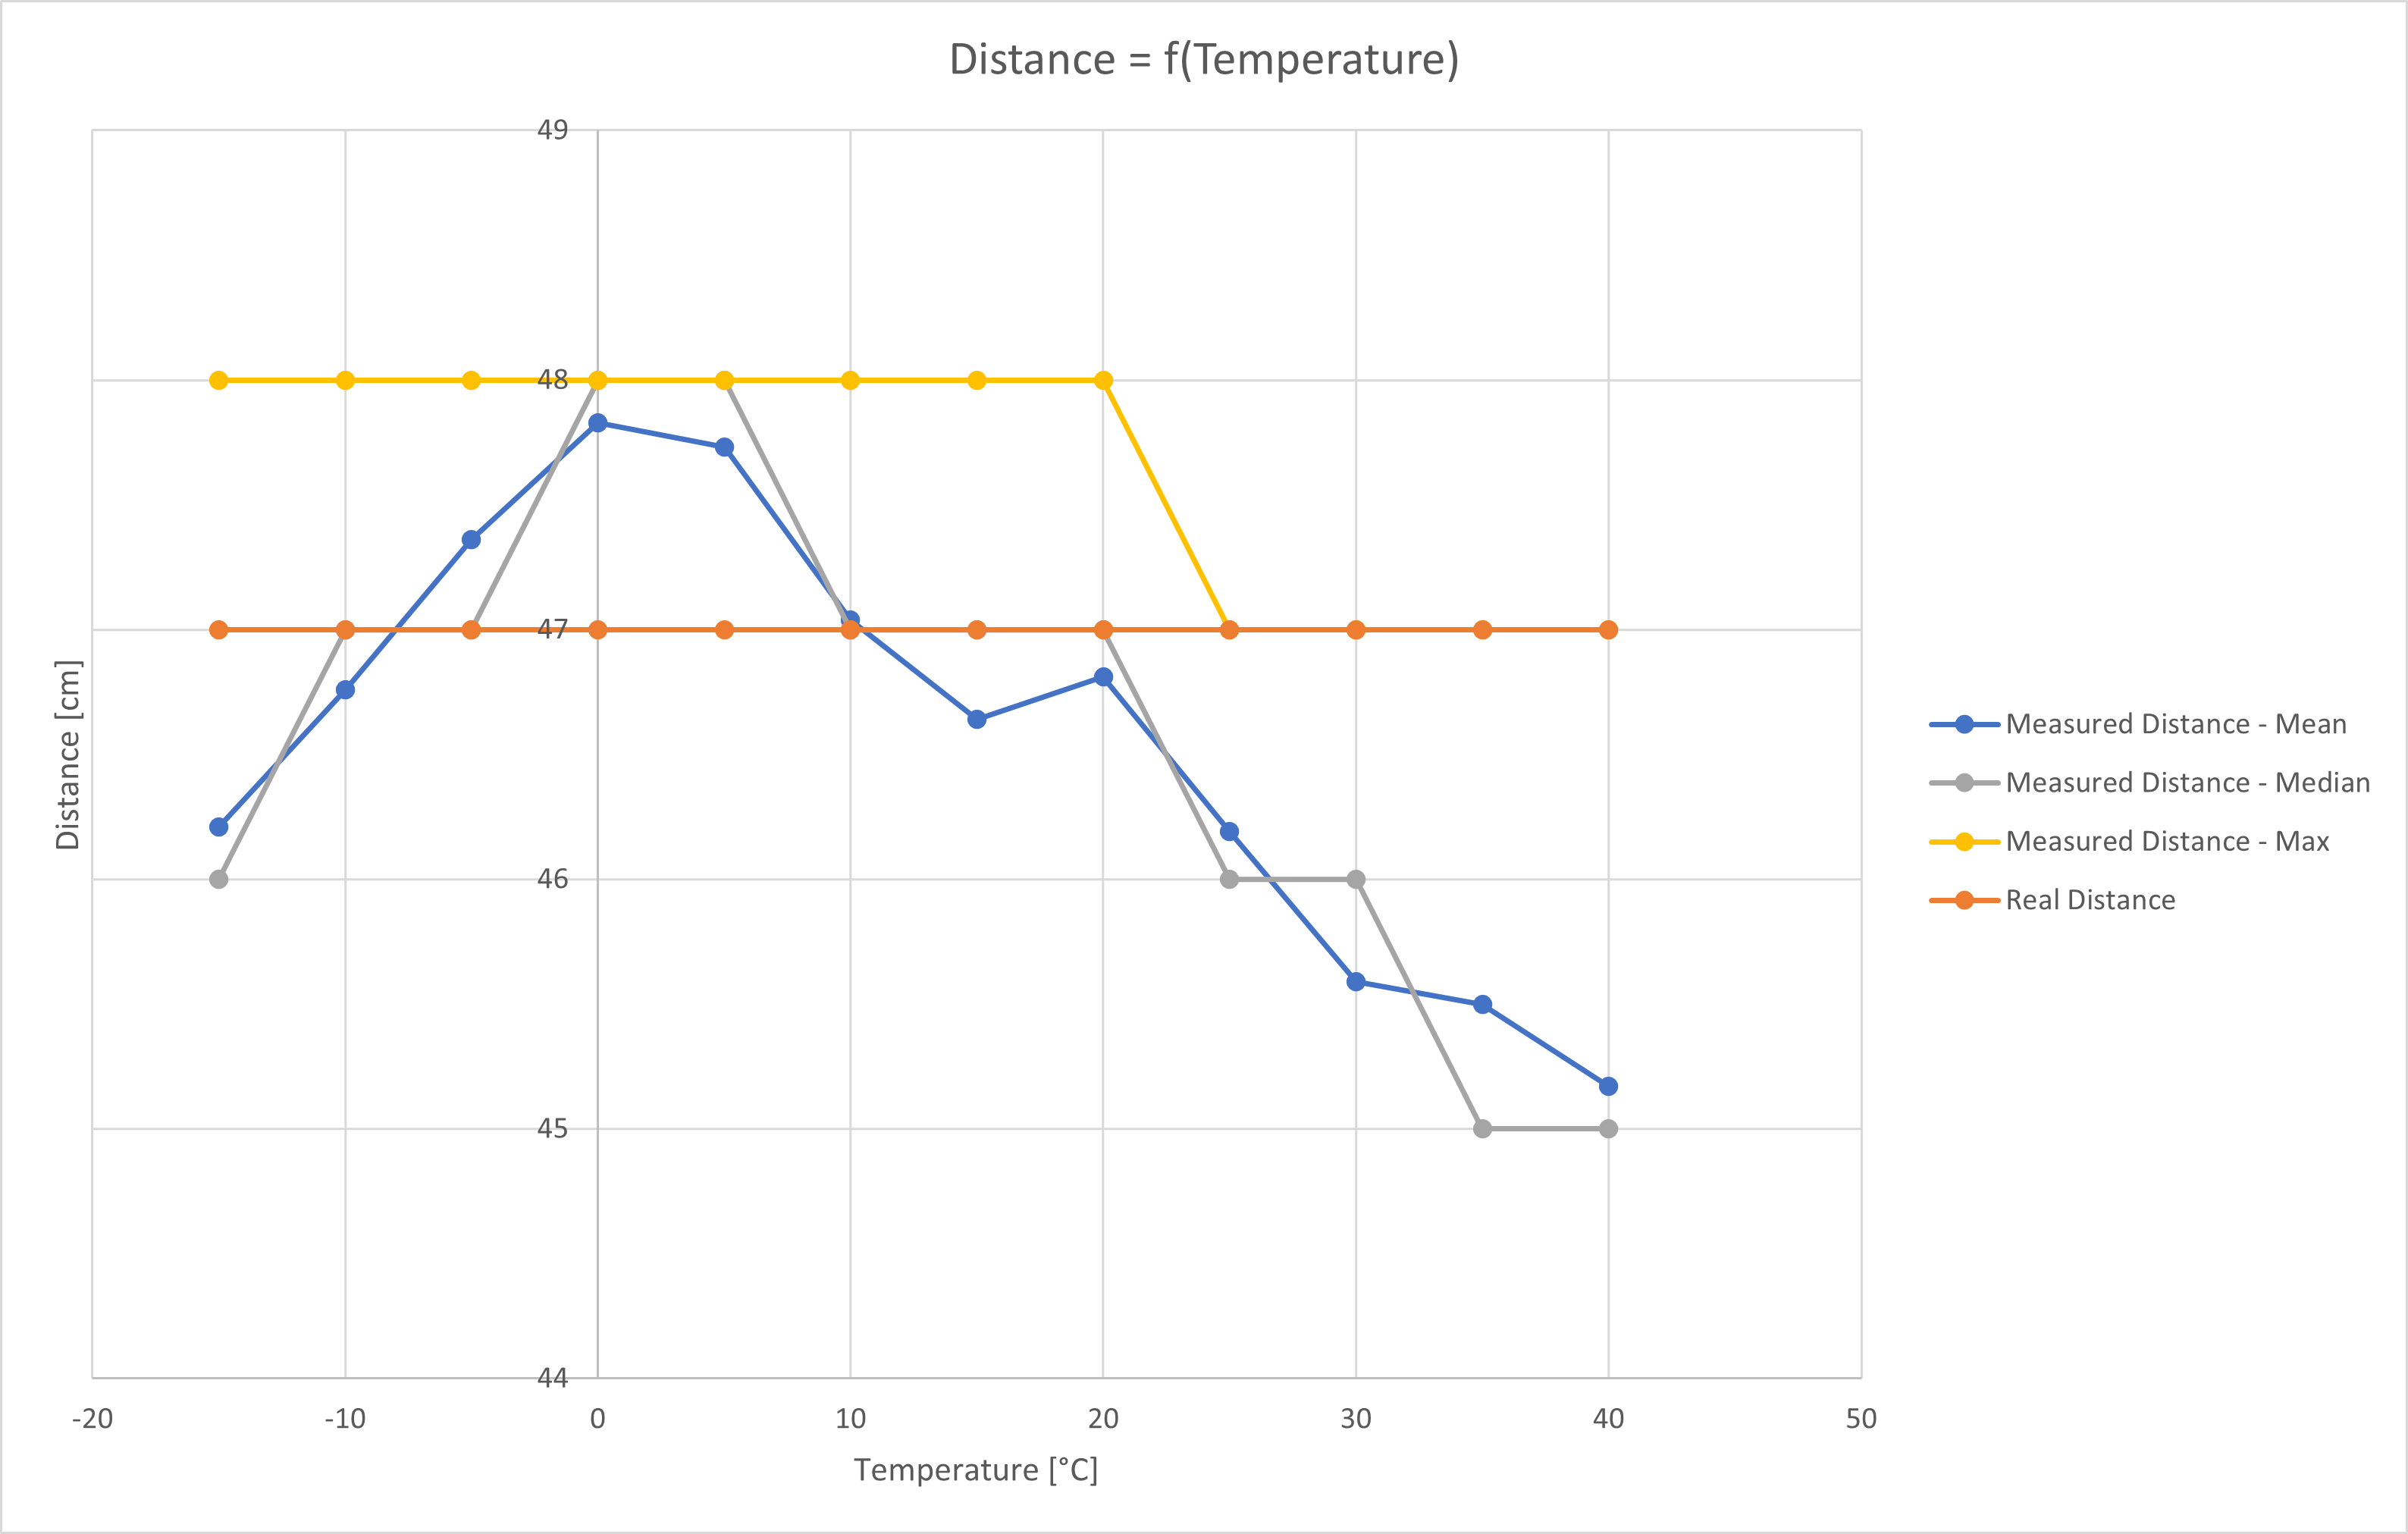
\includegraphics[width=0.8\textwidth]{Images/LiDAR/LiDAR_TempStabilityGraph.png}
    \caption{Graphe de stabilité en température du LiDAR}
    \label{fig:TempErrorGraph}
\end{figure}

Le test a été réalisé à partir d'une température de -15°C et non pas de -20°C. En effet, la chambre
climatique utilisée n'était pas en mesure d'atteindre cette consigne dans un temps raisonnable.\\
Les trois méthodes décrites dans le test précédent ont été reprises afin de mieux comprendre la
répartition des valeurs mesurées.

\subsubsection{Conclusion préliminaire} 

Il semblerait que le capteur soit relativement peu influencé par la variation de température. En
effet, en plus de sa résolution fixe de 1cm, nous avons une erreur typique de \textpm 2cm autour
de la valeur réelle.\\
Cependant, on constate tout de même que la moyenne et la médiane sont plus influencées que la méthode
du maximum. On peut ainsi conclure que le capteur est plutôt stable en température, surtout si on
utilise le maximum comme méthode de mesure.\par 
On peut considérer finalement que le capteur est fiable pour une mesure de référence et de hauteur
de neige prises à des températures différentes, comme cette différence est noyée dans sa précision
typique.

\subsection{Mesure de hauteur en laboratoire}

Maintenant que nous avons caractérisé ce capteur pour plusieurs situations, nous pouvons procéder aux
véritables mesures d'épaisseur en laboratoire. En effet, il faut à présent vérifier si la méthode de
calcul de la section \ref{sec:MethodeDeMesure} est réalisable en condition de laboratoire dans un premier
temps.

\subsubsection{Méthode}

Pour effectuer ce test, le capteur est placé dans le banc de test à une hauteur $h$ de 133cm au-dessus
du sol. L'angle $\alpha$ du LiDAR a été fixé à 60°, alors que l'angle $\beta$ est de 0°. Ces informations 
ont été fournies au programme de test afin de calculer des bons offsets. La figure \ref{fig:OffsetMes_Labo}
montre la préparation au test.\\
Le but est de mesurer tout d'abord une distance de référence au sol, sans aucun obstacle ni bruit de
mesure. Ensuite, une fois la plaque placée, on effectue quatre mesures différentes, la première sans
bruit puis avec un bruit graduel généré par les opérateurs.\\
L'obstacle utilisé est une plaque en mousse blanche de protection, d'une épaisseur de 6.6cm.

\begin{figure}[H]
    \centering
    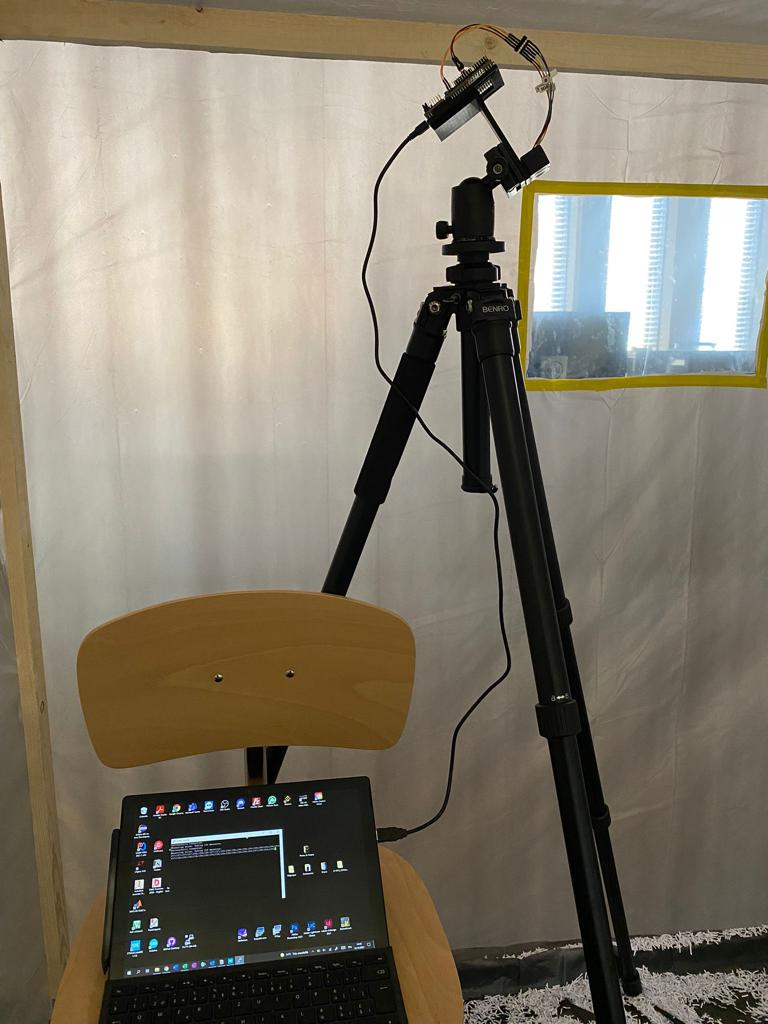
\includegraphics[width=0.5\textwidth]{Images/LiDAR/OffsetMes_InLab.jpeg}
    \caption{Mise en place du test de mesure d'épaisseur}
    \label{fig:OffsetMes_Labo}
\end{figure}

\subsubsection{Résultats du test}

\begin{figure}[H]
    \centering
    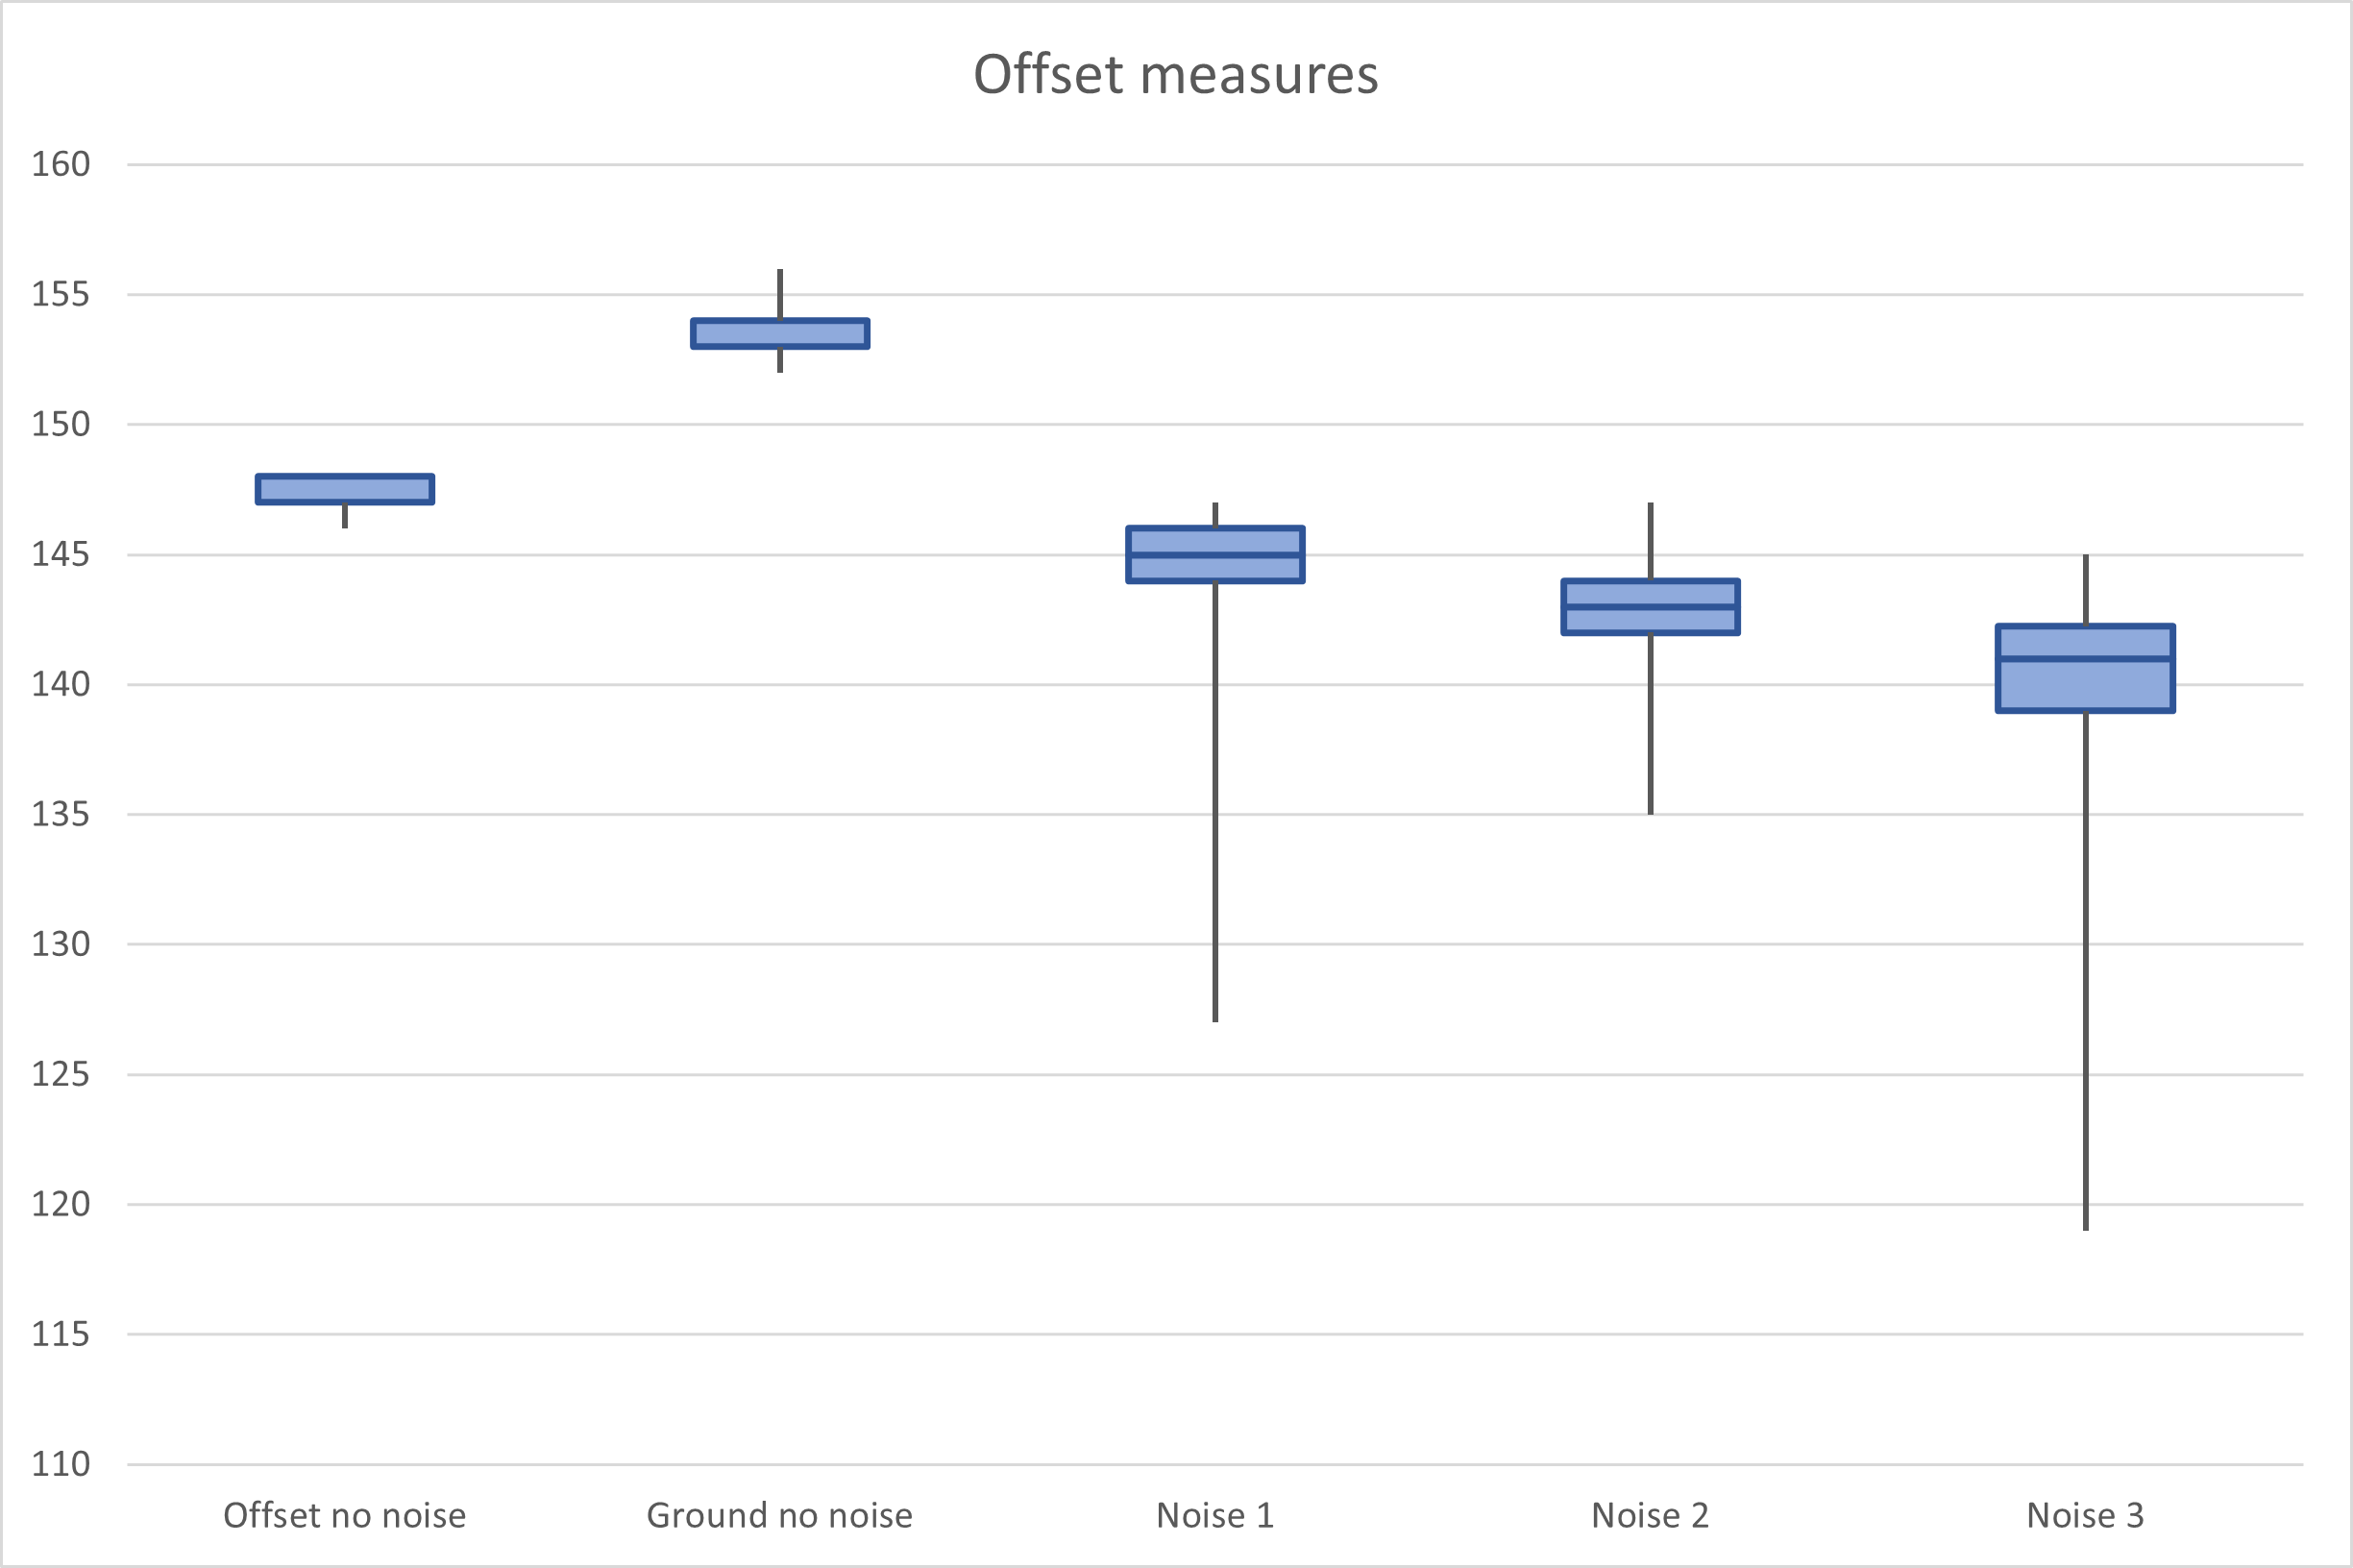
\includegraphics[width=0.8\textwidth]{Images/LiDAR/LiDAR_OffsetMes_Moustache.png}
    \caption{Boîte à moustache des mesures d'épaisseur}
    \label{fig:OffsetMes_Moustache}
\end{figure}

Il est important de noter que pour la série de mesure \emph{Noise 3}, la valeur maximale n'atteint
pas celle des autres séries. Cela est dû majoritairement au fait qu'une couche de 2cm de confettis
se sont accumulés sur la plaque au fil des mesures.

\begin{figure}[H]
    \centering
    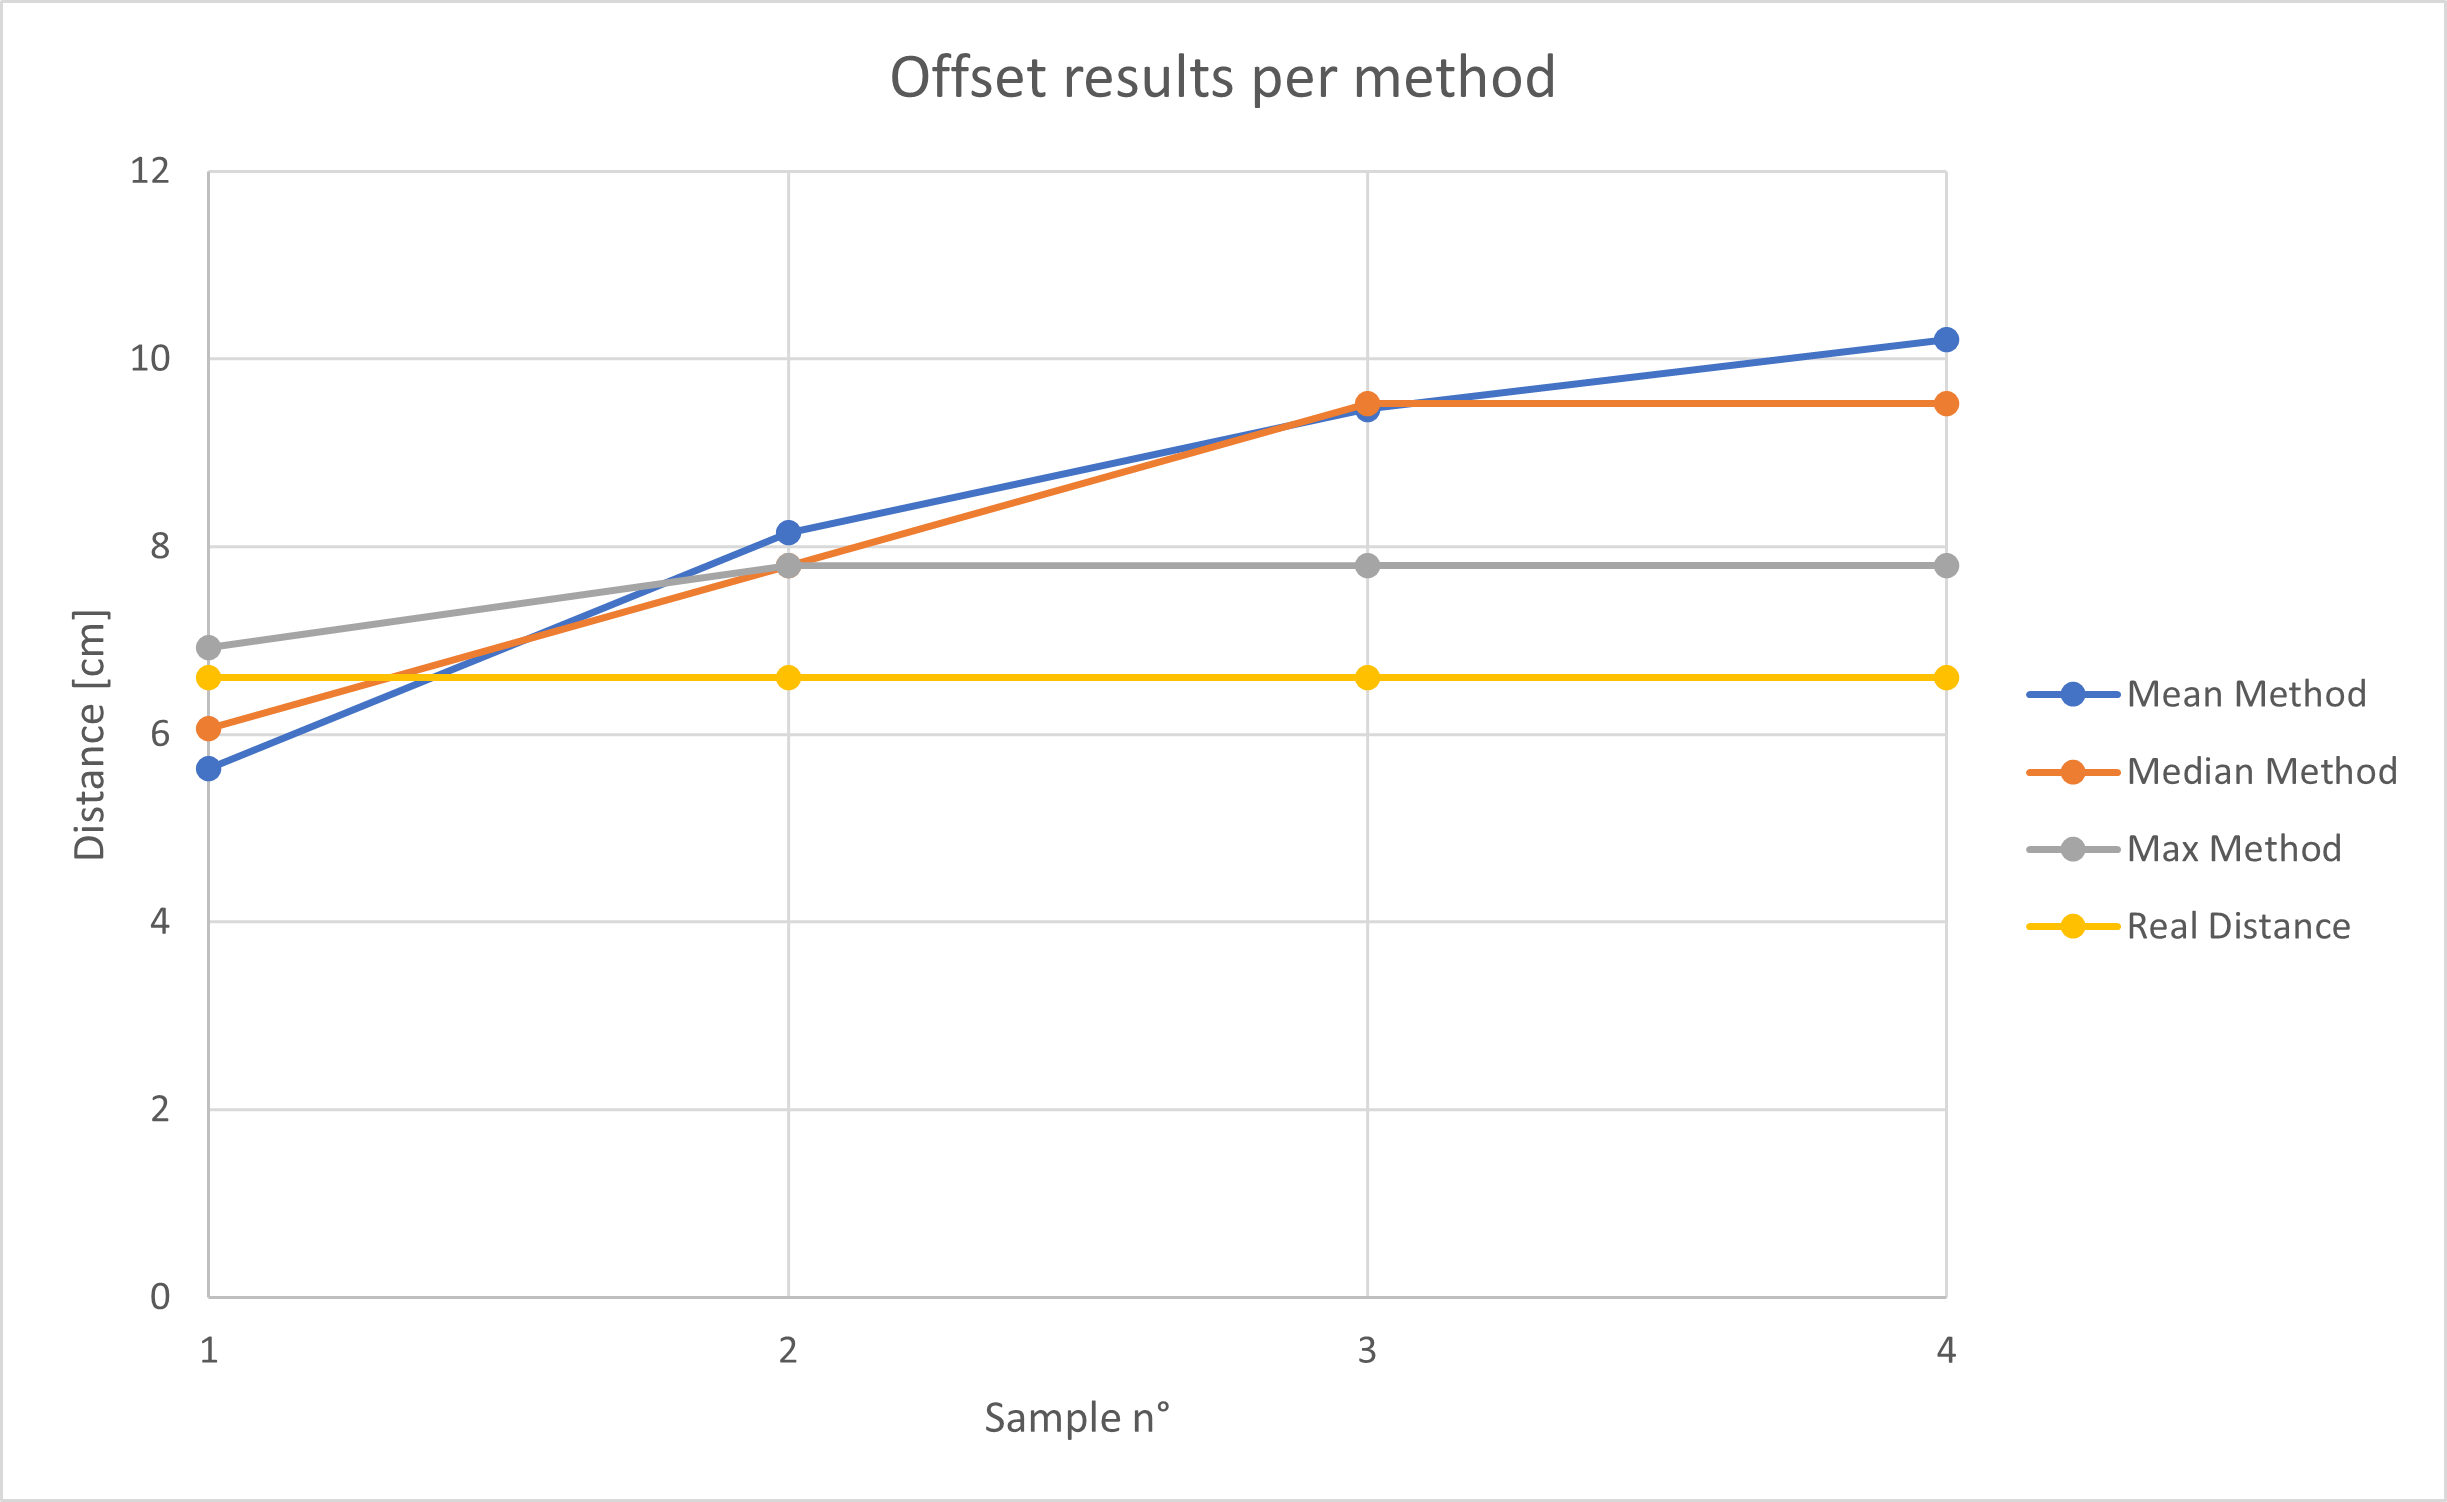
\includegraphics[width=0.8\textwidth]{Images/LiDAR/LiDAR_OffsetMes_PerMethods.png}
    \caption{Résultat des calculs d'offset par méthode}
    \label{fig:OffsetMes_PerMethod}
\end{figure}

\subsubsection{Conclusion préliminaire} 

Le graphe \ref{fig:OffsetMes_Moustache} montre la répartition des mesures effectuées sous la forme d'une
boîte à moustache. Cela permet de représenter facilement la répartition des mesures autour de la médiane.\\
On remarque sur les séries \emph{Noise 1} à \emph{Noise 3} que du bruit a bien été généré par les
opérateurs, ce qui n'est pas le cas pour les deux premières séquences de mesure. Hormis cela, le graphe
est très similaire aux tests dans un environnement perturbé, à la section \ref{fig:MesNoise}. On retrouve
en effet une médiane qui s'éloigne de plus en plus de la vraie distance, alors que le maximum s'approche
le plus de la réalité.\par
On voit sur la figure \ref{fig:OffsetMes_PerMethod} l'épaisseur calculée à l'aide de la méthode de la section
\ref{sec:MethodeDeMesure} pour les 3 solutions proposées, à savoir la moyenne, la médiane et le maximum. Ce
calcul d'offset a été réalisé pour les quatre séries de mesures à disposition, avec un bruit graduel. On 
peut ici conclure que la méthode du maximum est la plus proche de la réalité. Pour cette raison, elle sera
utilisée pour les tests sur le terrain.

\subsection{Mesure de hauteur en situation réelle}

Après avoir prouvé le fonctionnement du capteur en laboratoire, il est essentiel de le tester en conditions
réelles, sous la neige. Pour ce faire, des tests ont été réalisés la nuit du 3 au 4 décembre 2021 à Ayent.
Un boitier temporaire a été confectionné afin de protéger le LiDAR et la carte de développement des 
précipitations.

\subsubsection{Méthode}

Le boitier a été installé sur un trépied à 140cm au-dessus du sol, sous un couvert, à l'abri de la majorité
des flocons. Le LiDAR pointe vers le sol avec un angle de 45° par rapport à la verticale, donnant une
distance de 197cm entre le capteur et la route. Les données récoltées sont enregistrées via un câble 
USB sur un ordinateur.\\
Le but est de mesurer des épaisseurs de neige en partant de 0cm (la route a été nettoyée au préalable)
afin de mettre à l'épreuve l'efficacité du capteur et de nos méthodes de mesure. Chaque mesure d'épaisseur 
est réalisée chaque 30 secondes, et ce pendant plus d'une heure. En parallèle, une double-mètre est posé 
dans la neige afin de relever périodiquement la hauteur de neige présente sur la route. Une mesure
qualitative du débit de neige est aussi effectuée. La figure \ref{fig:RealTest_Setup} montre la mise en
place du test. Le double-mètre et l'ordinateur ne sont pas visibles ici.

\begin{figure}[H]
    \centering
    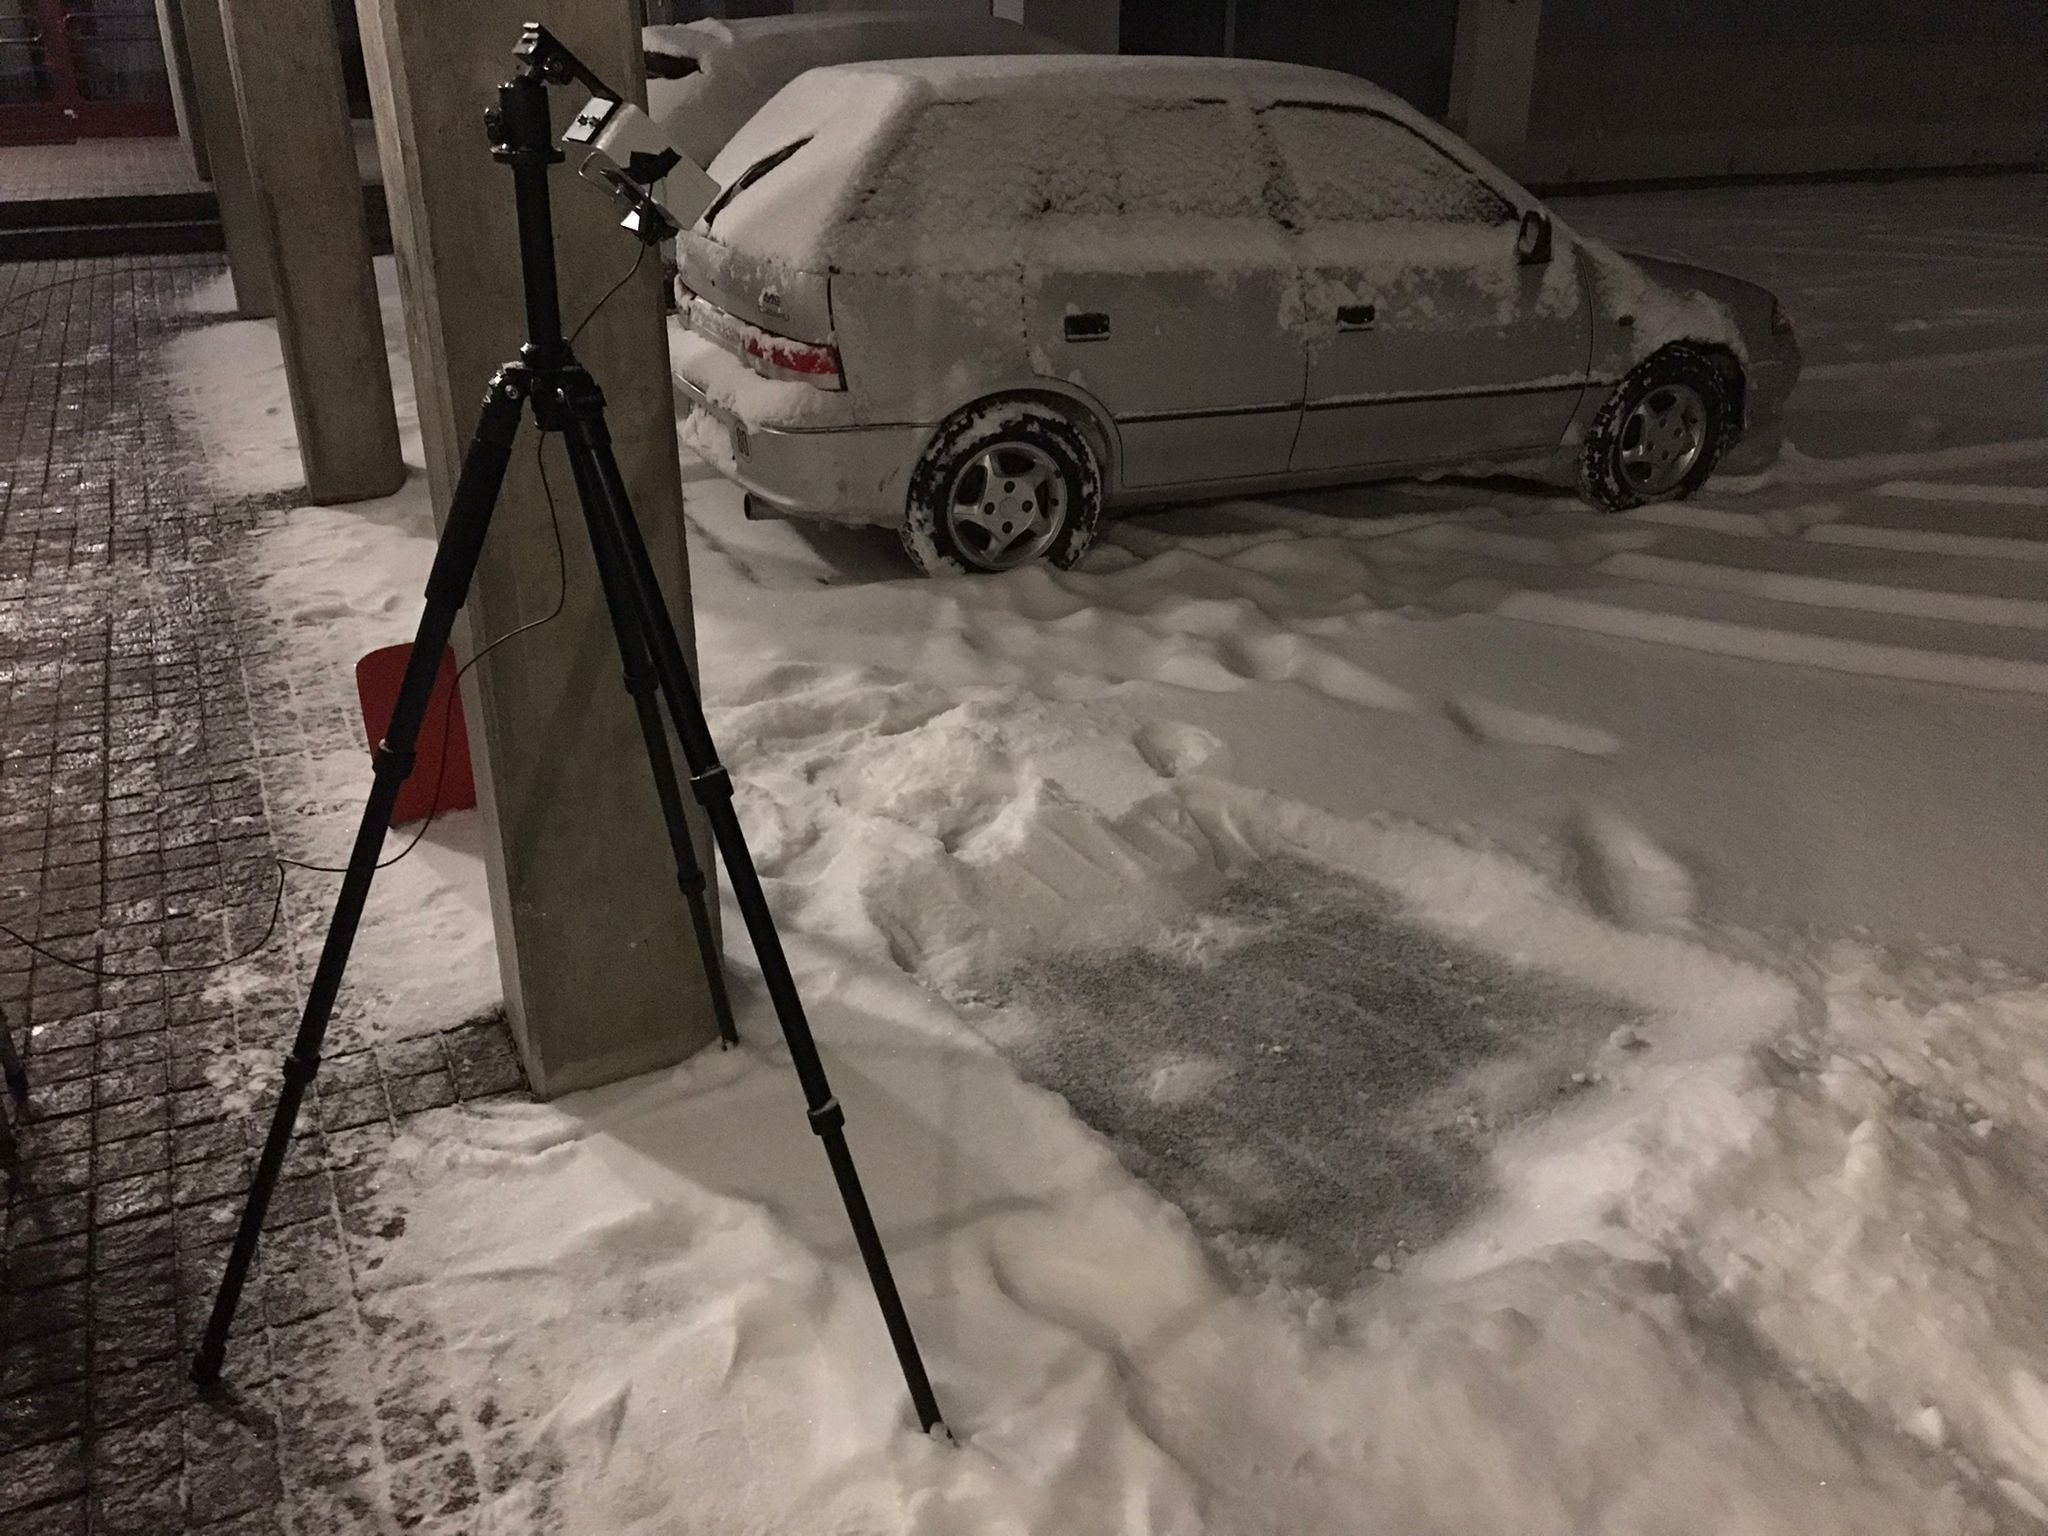
\includegraphics[width=0.75\textwidth]{Images/LiDAR/ReadTests_Setup.jpeg}
    \caption{Mise en place du test en condition réelle}
    \label{fig:RealTest_Setup}
\end{figure}

\subsubsection{Résultats du test}

\begin{table}[H]
    \centering
    \begin{tabular}{|c|c|c|c|c|}
        \hline
        Mesure n° & Hauteur réelle [cm] & Hauteur mesurée [cm] & Type de précipitation & Heure \\
        \hline\hline
        1 & 0 & 0 & Petits flocons & 04h28 \\
        \hline
        2 & 0.5 & 0.71 & Petits flocons & 04h39 \\
        \hline
        3 & 0.8 & 1.41 & Quelques gros flocons & 04h48 \\
        \hline
        4 & 1.5 & 1.41 & Quelques gros flocons & 05h00 \\
        \hline
        5 & 2 & 2.12 & Quelques gros flocons & 05h08 \\
        \hline
        6 & 2.5 & 2.12 & Quelques gros flocons & 05h14 \\
        \hline
        7 & 2.8 & 2.86 & Quelques gros flocons & 05h21 \\
        \hline
        8 & 3 & 2.86 & Quelques gros flocons & 05h32 \\
        \hline
        
    \end{tabular}
    \caption{Mesures relevée lors du test}
    \label{table:SnowingState}
\end{table}

\begin{figure}[H]
    \centering
    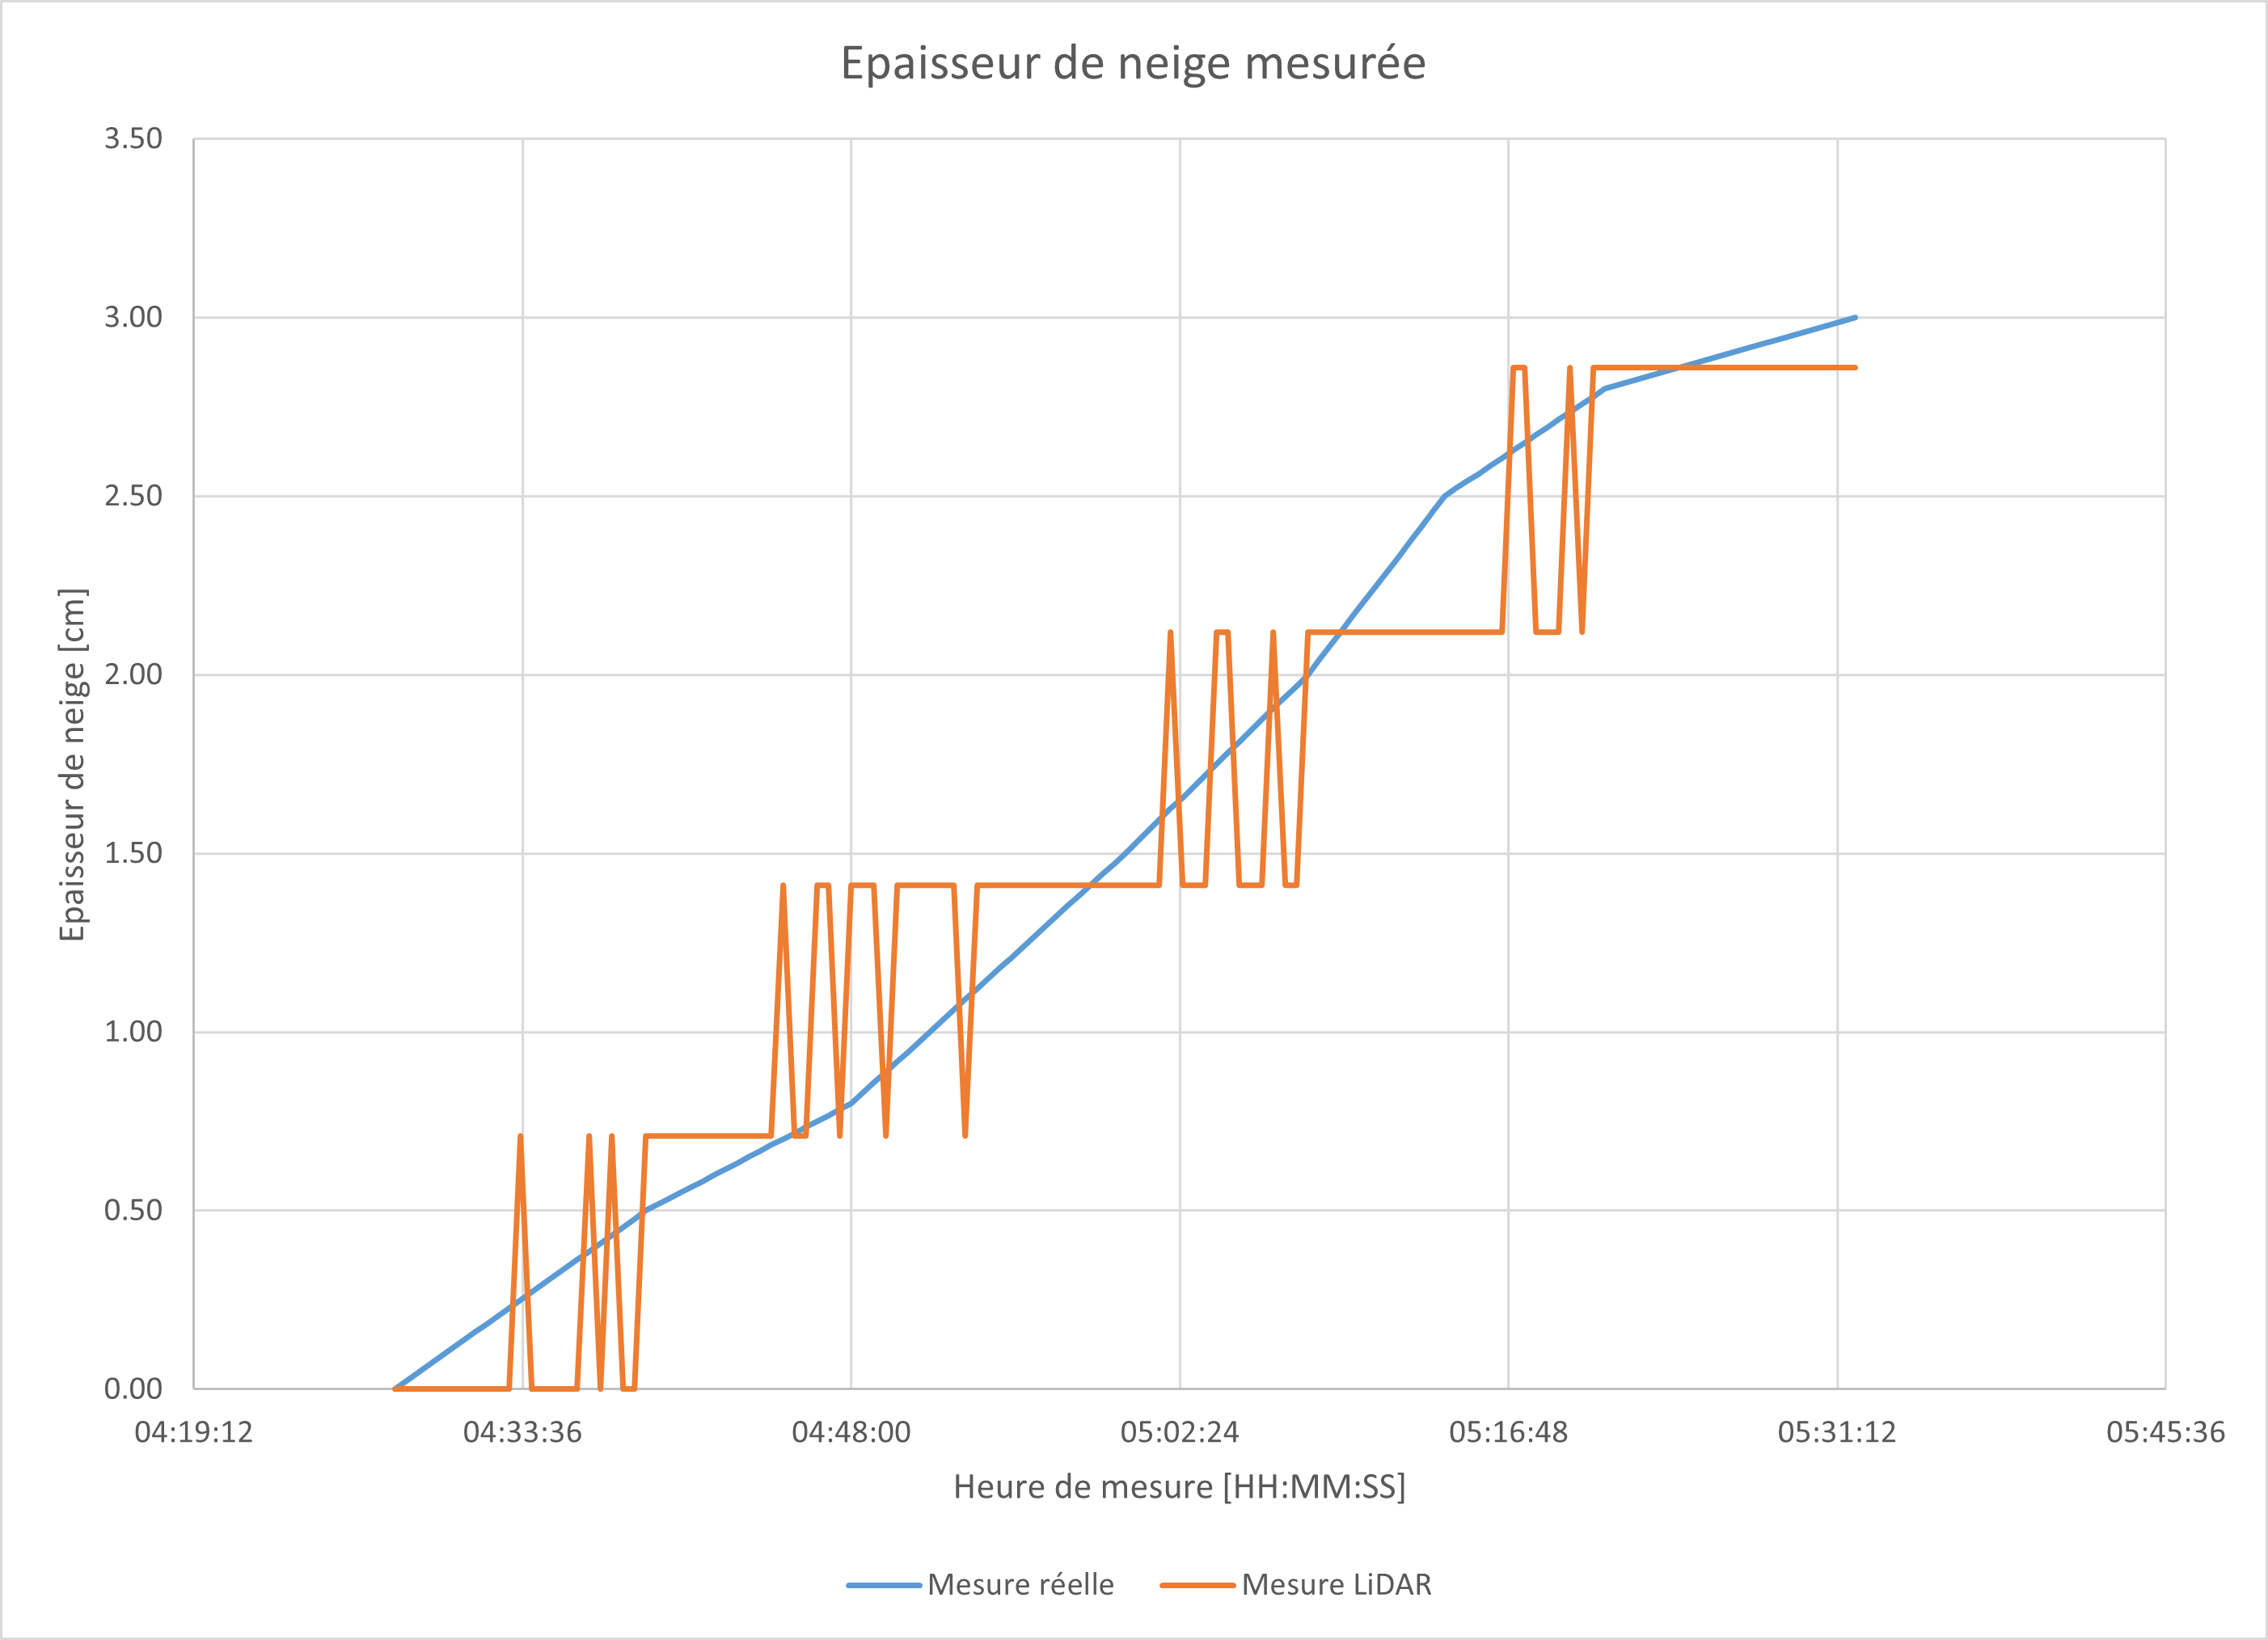
\includegraphics[width=0.75\textwidth]{Images/LiDAR/ReadTests_Results.png}
    \caption{Résultat des mesures effectuées}
    \label{fig:RealTest_Results}
\end{figure}

La température lors des mesures oscillait entre -2°C et 0°C, sans aucun vent.\par 
Afin de réaliser la courbe \emph{Mesure réelle} de la figure \ref{fig:RealTest_Results}, une interpolation
linéaire a été utilisée entre les différents points de mesure.

\subsubsection{Conclusion préliminaire} 

Après avoir passé plusieurs heures dans un froid glacial à mettre à l'épreuve notre projet, nous avons 
enfin pu obtenir des résultats.\\
Le tableau \ref{table:SnowingState} montre les différentes heures de mesures, mettant notamment en évidence
l'erreur entre la valeur réelle et mesurée. Malgré une légère oscillation lors d'un changement proche
de valeur (figure \ref{fig:RealTest_Results}), on peut conclure que le LiDAR arrive bel et bien à mesurer 
une hauteur de neige, et ce depuis le sol.\par 
On constate par la même occasion que le pas de mesure du capteur dépend effectivement de son angle par 
rapport à la verticale.

\chapter{Computer Vision}
La \emph{Computer Vision} (ou vision par ordinateur) comprend l'acquisition, l'analyse et
le traitement des images numériques pour comprendre et extraire des données, informations
ou décisions.\\
Les applications et possibilités de ce domaine sont pour ainsi dire, infinie.

\section{Défis liés à la mesure en extérieur}
La principale difficulté de la mesure de neige par \emph{Computer Vision} est lié au fait
qu'il neige. Les caméras embarquées sont souvent de mauvaise qualité, et les débits
sont mauvais à cause des processeurs embarqués qui sont limités en puissance de calcul.

\begin{figure}[H]
    \centering
    
\includegraphics[width=0.4\textwidth]{Images/computer_vision/perfect_snow.jpg}
    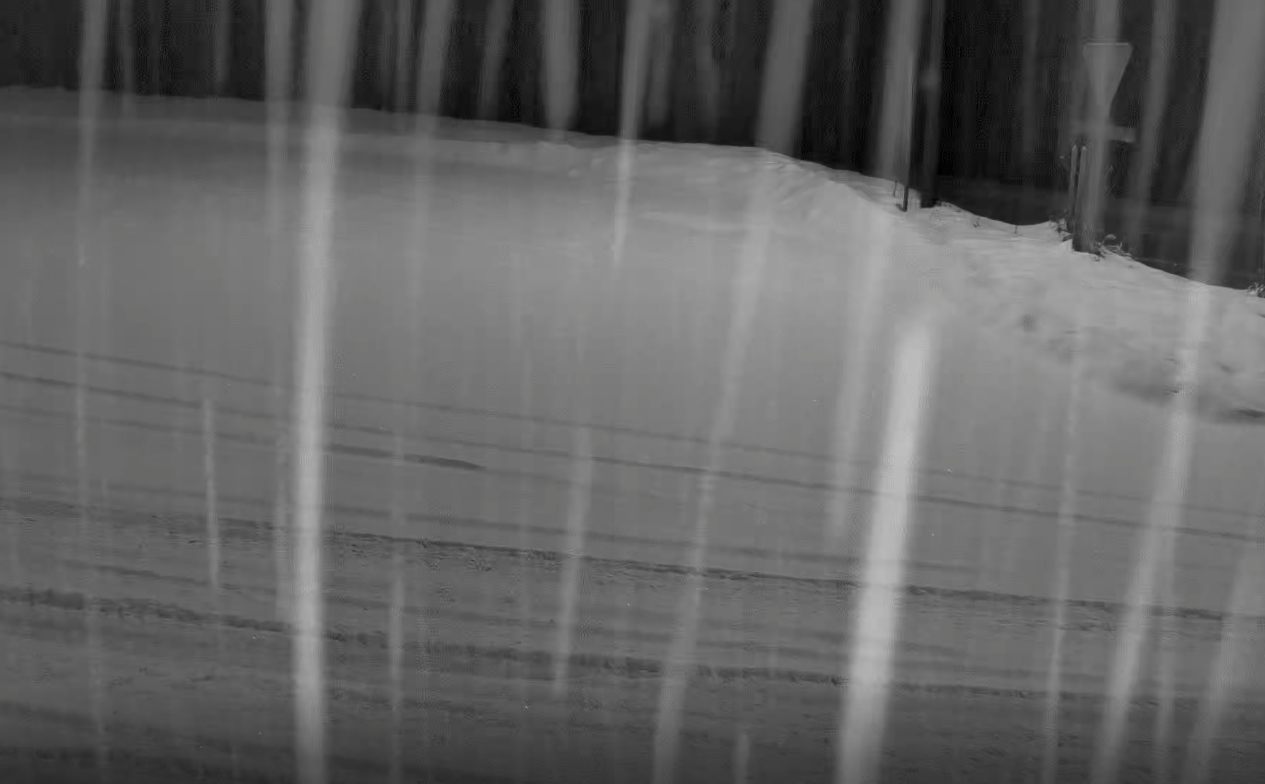
\includegraphics[width=0.4\textwidth]{Images/computer_vision/real_snow.png}
    \caption[Comparaison image de neige HD et cas concret]{Comparaison entre une image idéale \footnotemark[1] et un cas concret\footnotemark[2]}
    \label{fig:Snow comparison}
\end{figure}
\footnotetext[1]{Wallpaper from WallpaperCave, by caveman, https://wallpapercave.com/w/scDoVwf
(last accessed: 20 January 2022)}
\footnotetext[2]{VibroSnow camera, implemented at route du Pralan, Ayent, Suisse}

\noindent
Il faut donc trouver une méthode ne demandant pas trop de ressources de calcul, et pouvant fournir
des résultats utiles pour informer sur l'état des routes.

\section{Applications pour la mesure de neige}
Les possibilités de la \emph{Computer Vision} étant vaste, plusieurs méthodes ont été discutées.

\newpage

\subsection{Mesure de niveau sur une règlette}
Les mesures de niveau de neige manuel se font déjà avec une réglette plantée dans la neige.

\begin{figure}[H]
    \centering
    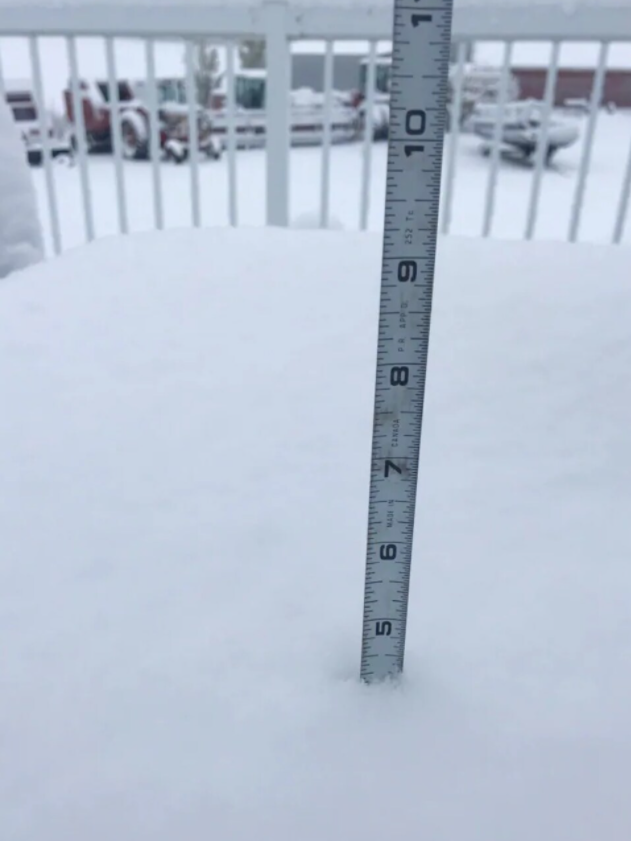
\includegraphics[width=0.3\textwidth]{Images/computer_vision/snow_meter.PNG}
    \caption[Mesure de neige à la règle]{Mesure d'environ 4.5 pouces de neige à Manitoba, Canada\footnotemark[1]}
    \label{fig:Snow meter}
\end{figure}
\footnotetext[1]{Image by Jerry Zachedniak, https://ici.radio-canada.ca/nouvelle/1338531/hiver-tempete-parc-mont-riding
(last accessed: 20 January 2022)}
\noindent
La mesure pourrait être réalisé en plaçant la caméra en face de la règlette.
Deux méthodes sont possibles :
\begin{description}
    \item[Avoir une règlette graduée] \hfill \\
    et compter le nombre de graduation encore visible pour déterminer la hauteur de neige.
    \item[Avoir un piquet d'une taille connue] \hfill \\
    comparer la hauteur de ce piquet au nombre de pixel quand il n'y a pas de neige,
    puis mesurer le nombre de pixels non-ensevelis pour mesurer la hauteur de neige.
\end{description}
\noindent
Cependant mesurer une règlette peut paraître simple d'un point de vue de l'implémentation,
mais présente plusieurs désavantages lors du fonctionnement:

\begin{description}
    \item[Il faut déneiger devant la caméra et la règlette] \hfill \\
    demandant probablement à un ouvrier de descendre de son chasse-neige pour déneiger l'installation.
    \item[L'installation ne doit pas être trop proche d'une route] \hfill \\ 
    de risque d'être ensevelie ou endommagée lors du passage d'un chasse-neige.
    \item[Si on utilise une règlette graduée] \hfill \\ 
    il faut s'assurer d'avoir un matériau surlequel la neige ne colle pas ou 
    ne réfléchis pas trop la lumière du soleil.
    \item[L'utilisation d'un piquet peut demander l'usage d'une intelligence artificielle] \hfill \\
    pour reconnaitre le piquet d'autres objets (p. ex.: arbres, lampadaires, ...) \cite{SnowTimeLapse}%\footnotemark[2])
    Cela demanderait trop de puissance de calcul pour un système embarqué basse consommation.
    Une autre solution serait de calibrer chaque installation pour reconnaître le piquet.
    Cependant la caméra étant intégrée dans un système embarqué, cette calibration serait certainement
    fastidieuse et demanderait une interface utilisateur supplémentaire pour la réaliser.
\end{description}
%\footnotetext[2]{\emph{Snow Depth Measurement via Time Lapse Photography and Automated Image Recognition},
%by Kevin S. J. Brown and Steven R. Fassnacht at Colorado State University,
%Departement of Ecosystem Science and Sustainability, 2019, http://www.codos.org/\#lit}
\newpage

\subsection{Mesure de niveau par Stéréovision}
La Stéréovision est une méthode de mesure se servant d'images provenant de plusieurs point de vue.
Typiquement, deux caméras côte à côte, peuvent mesurer des profondeurs comme des yeux.

\begin{figure}[H]
    \centering
    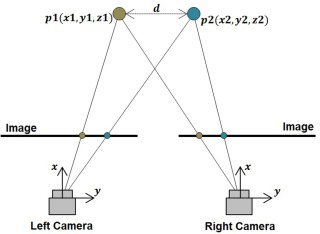
\includegraphics[width=0.5\textwidth]{Images/computer_vision/stereovision.jpg}
    \caption[Schéma de principe stéréovision]{Schéma de principe de mesure de distance par stéréovision}
    \label{fig:Stereovision}
\end{figure}
\noindent
Beaucoup de caméra spécialisée dans la reconnaissance d'image par Intelligence artificielle utilise se principe
pour estimer les distances (ex: OpenCV OAK cameras).
Cette méthode demande trop de puissance de calcul pour un système embarqué basse consommation et ne fournit
pas de résultat suffisamment précis pour mesurer une couche de neige.
\newpage

\subsection{Mesure du débit de chute de neige}
Une mesure simple et rapide est d'estimer le débit de chute de neige en isolant les flocons.
\begin{figure}[H]
    \centering
    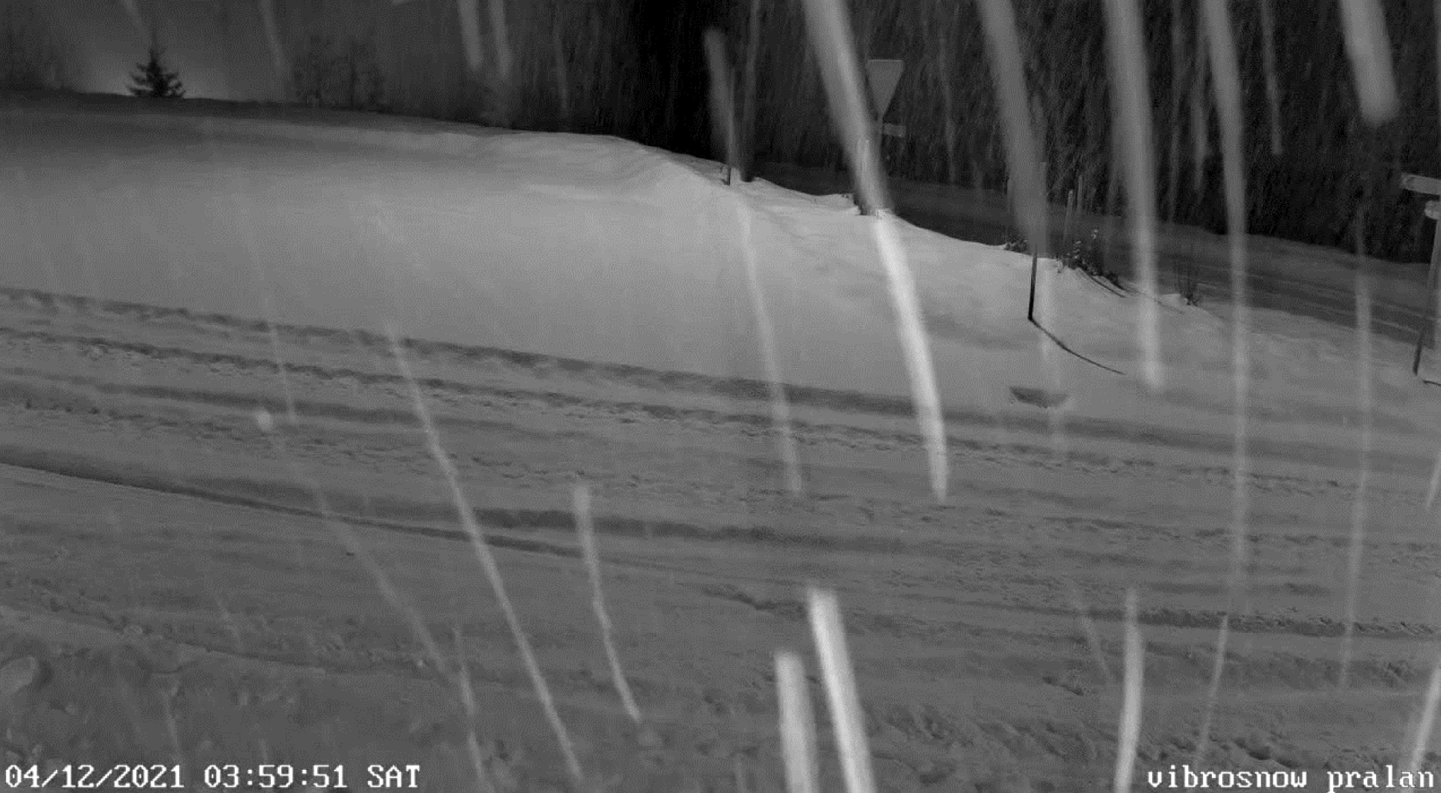
\includegraphics[width=0.35\textwidth]{Images/computer_vision/snow_cam.png}
    
\includegraphics[width=0.35\textwidth]{Images/computer_vision/snowfall.png}
    \caption[Comparaison image source et bruit sur image]{Image source de la caméra VibroSnow\footnotemark[1] et image avec les flocons isolés}
    \label{fig:Snowfall}
\end{figure}
\footnotetext[1]{VibroSnow camera, implemented at route du Pralan, Ayent, Suisse}
\noindent
Cette mesure, en parrallèle à une mesure de hauteur de neige, permettrait d'estimer 
l'augmentation de cette hauteur au fil du temps. Fournissant ainsi une information supplémentaire
aux services de déneigement.

\subsection{Détection de route enneigée}
Étant donné que la mesure de hauteur de neige par \emph{Computer Vision} serait trop complexe
pour un système embarqué basse consommation, détecter si la route est enneigée ou non
permettrait de fournir une redondance à une mesure de hauteur de neige fournie par un autre capteur.
Si la petite zone mesurée par le capteur se retrouve mal déneigée, ou qu'un objet, comme un caillou, mal placé
fausse la mesure du capteur, savoir si le segment de route est enneigé ou non permettrait d'éliminer ces erreurs.

\subsection{Méthodes retenues}
Les méthodes retenues pour ce projet de recherche sont \textbf{la mesure du débit de chute de neige}
et \textbf{la détection de route enneigée}. Elles peuvent fournir des informations pertinentes
pour le déneigement, tout en demandant relativement peu de puissance de calcul.
\newpage

\section{Implémentation}
Pour tester les algorithmes de mesure avec des vidéos sur le terrain,
Dr. Mudry Pierre-André et M. Matter Fabien nous on aimablement laissé accès à
la caméra de notre projet parent \emph{VibroSnow\cite{VibroSnow}} et nous
les remercions énormément.

\subsection{Récupération des vidéos}
La caméra de \emph{VibroSnow} détecte le passage d'objet (voitures, chute de neige,...) et
enregistre une vidéo qui est ensuite transmise à un serveur \emph{Windows}.
Bien que l'accès aux vidéos nous a été donné, nous ne pouvons pas aller chercher les vidéos
directement sur le serveur \emph{Windows} car il est utilisé pour d'autres projets auxquels nous
n'avons pas accès.\\
Il a donc fallu créer un script \emph{Powershell}, transferant chaque jour les vidéos
cumulées sur le serveur \emph{Windows} vers un serveur auquel nous avons accès.
Un \emph{Raspberry Pi} a été mis en place comme serveur pour récuperer les vidéos.

\subsection{Mesure du débit de chute de neige}
La méthode utilisée pour détecter les chutes de neige se décompose ainsi :
\begin{description}
    \item[Soustraction de deux images] \hfill \\
    pour isoler les éléments qui ont bougé entre les deux images
    \item[Seuillage des niveaux de blancs sur l'image] \hfill \\
    pour accentuer les chutes de neige
    \item[Calcul du ratio de pixels blancs] \hfill \\
    pour avoir un nombre correspondant au débit de chute de neige    
\end{description}

\begin{figure}[H]
    \begin{subfigure}{.45\textwidth}
        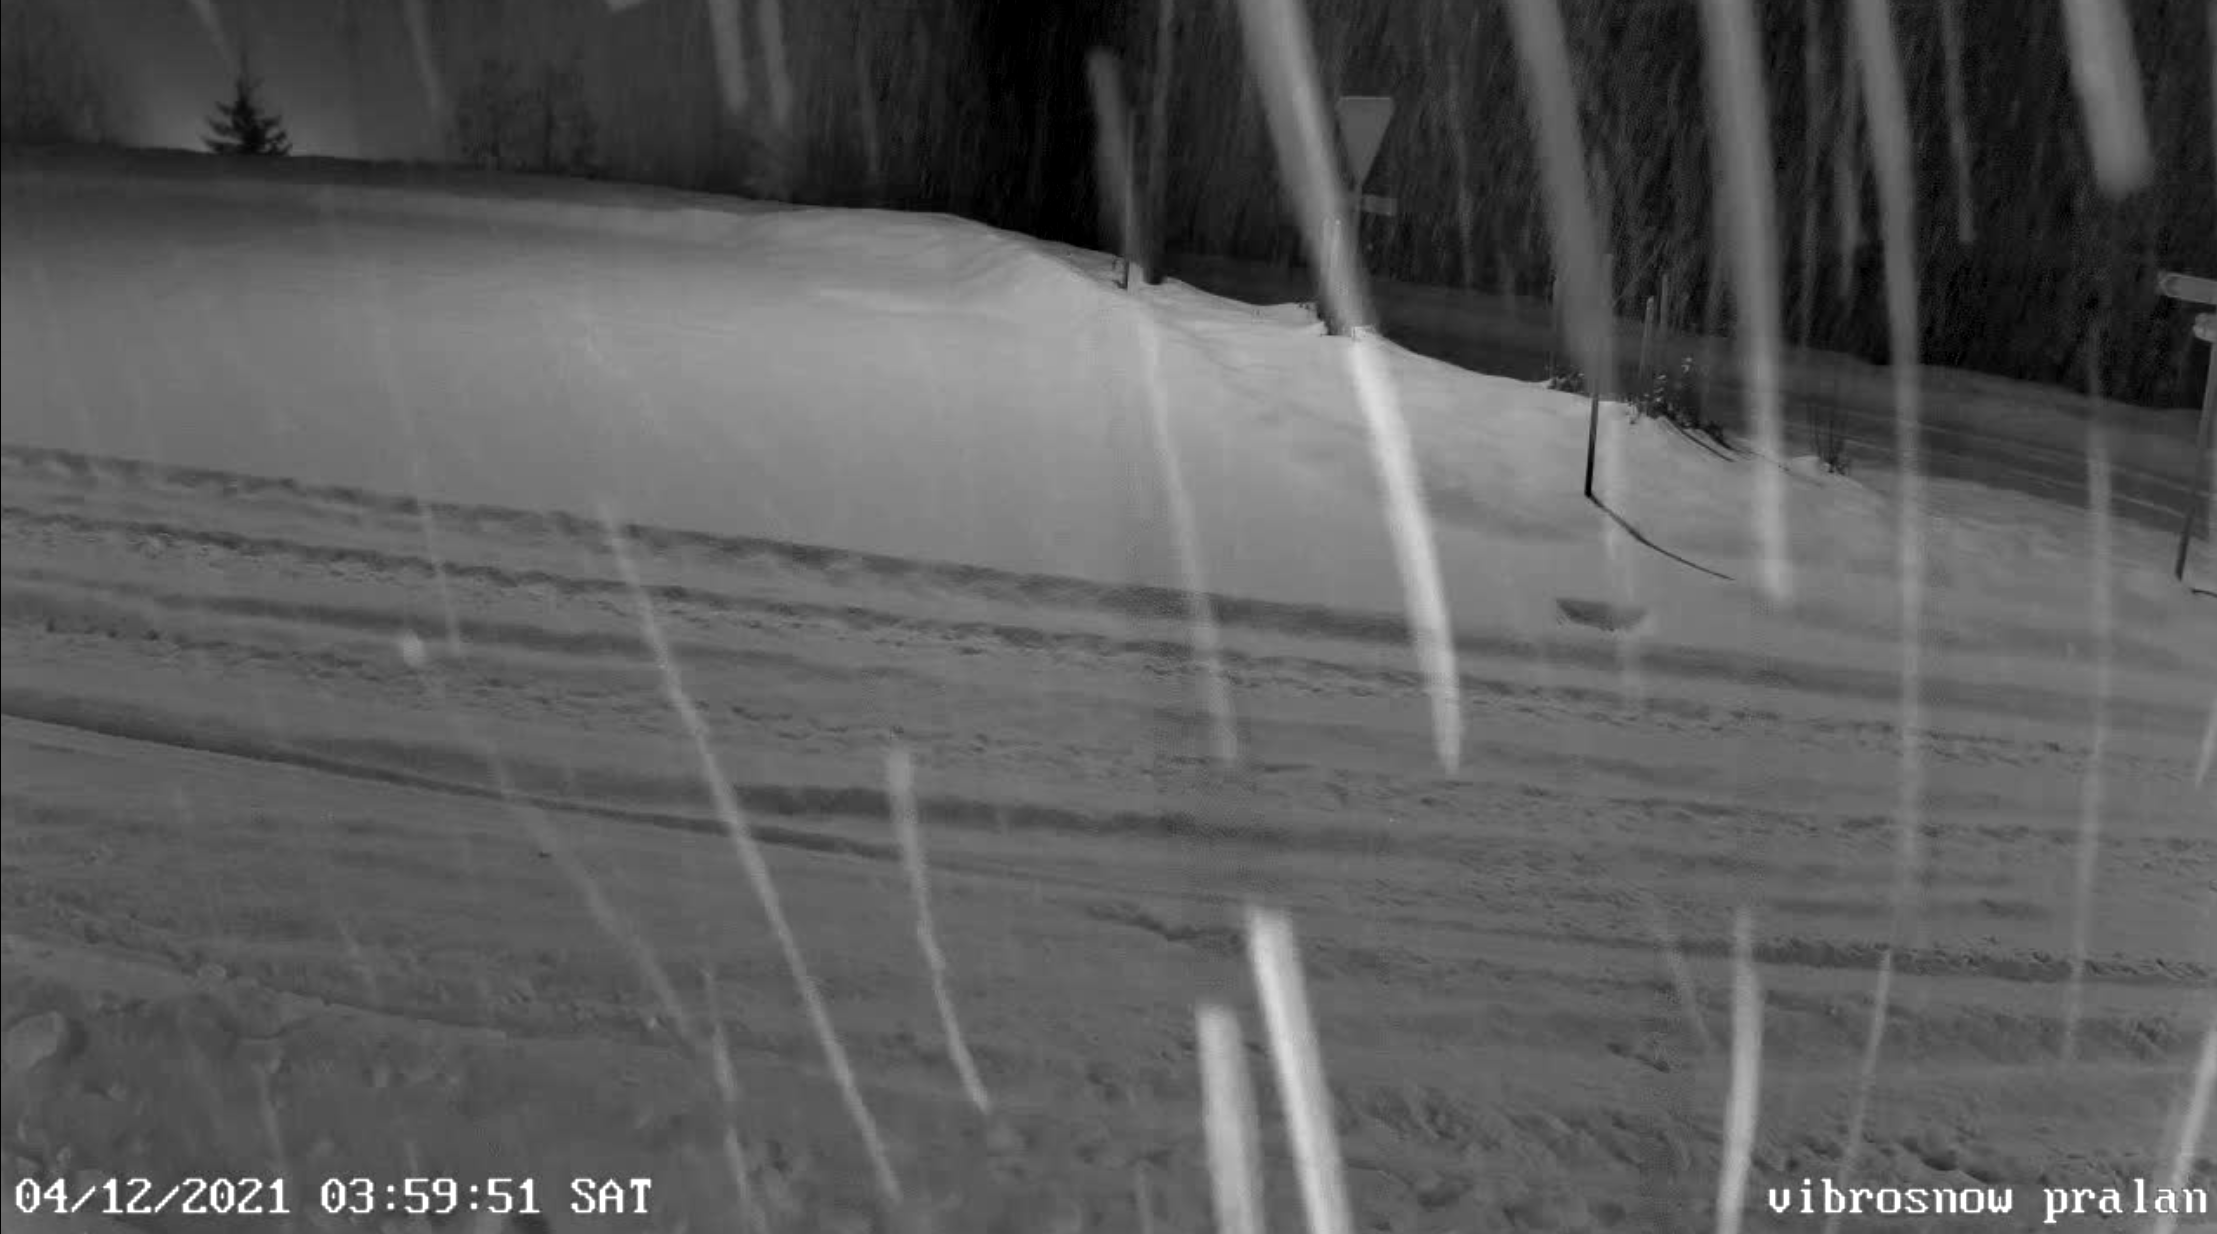
\includegraphics[width=\linewidth]{Images/computer_vision/snowfall/original.png}
        \caption{Image originale}
        \label{fig:Snowfall_original}
    \end{subfigure}
    \hfill
    \begin{subfigure}{.45\textwidth}
        
\includegraphics[width=\linewidth]{Images/computer_vision/snowfall/noise.png}
        \caption{Image avec neige isolée}
        \label{fig:Snowfall_noise}
    \end{subfigure}
    \hfill
    \centering
    \begin{subfigure}{.45\textwidth}
        
\includegraphics[width=\linewidth]{Images/computer_vision/snowfall/snowfall.png}
        \caption{Image seuillée avec calcul du ratio de pixels blancs (9.05\% ici)}
        \label{fig:Snowfall_thres}
    \end{subfigure}
    \caption{Étapes de la mesure de débit de chute de neige}
    \label{fig:Snowfall_algorithm}
\end{figure}
\newpage

\subsection{Détection de route enneigée}
Deux méthodes ont été testées pour détecter si la route est enneigée ou non.\\
La première réalise un simple seuillage des niveaux de blancs, et un calcul
du ratio des pixels blancs sur l'image. On récupère plusieurs images et on
calcul la moyenne du ratio de blanc sur toute les images.
Cette moyenne est ensuite comparée à une moyenne similaire réalisée sur une
vidéo de la route déneigée, en vérifiant qu'on se trouve au même moment de
la journée (jour/nuit, matin/après-midi).\\
La deuxième est identique, à l'exception d'une suppression du bruit réalisée
avant le seuillage. Cette suppresion du bruit reprends la méthode d'isolation
de neige utilisée pour mesurer le débit de chute de neige et soustrait cette image
de bruit à l'image originale. Cette méthode demande un peu plus de calculs mais peut
potentiellement générer un résultat plus fiable.

\begin{figure}[H]
    \begin{subfigure}{.45\textwidth}
        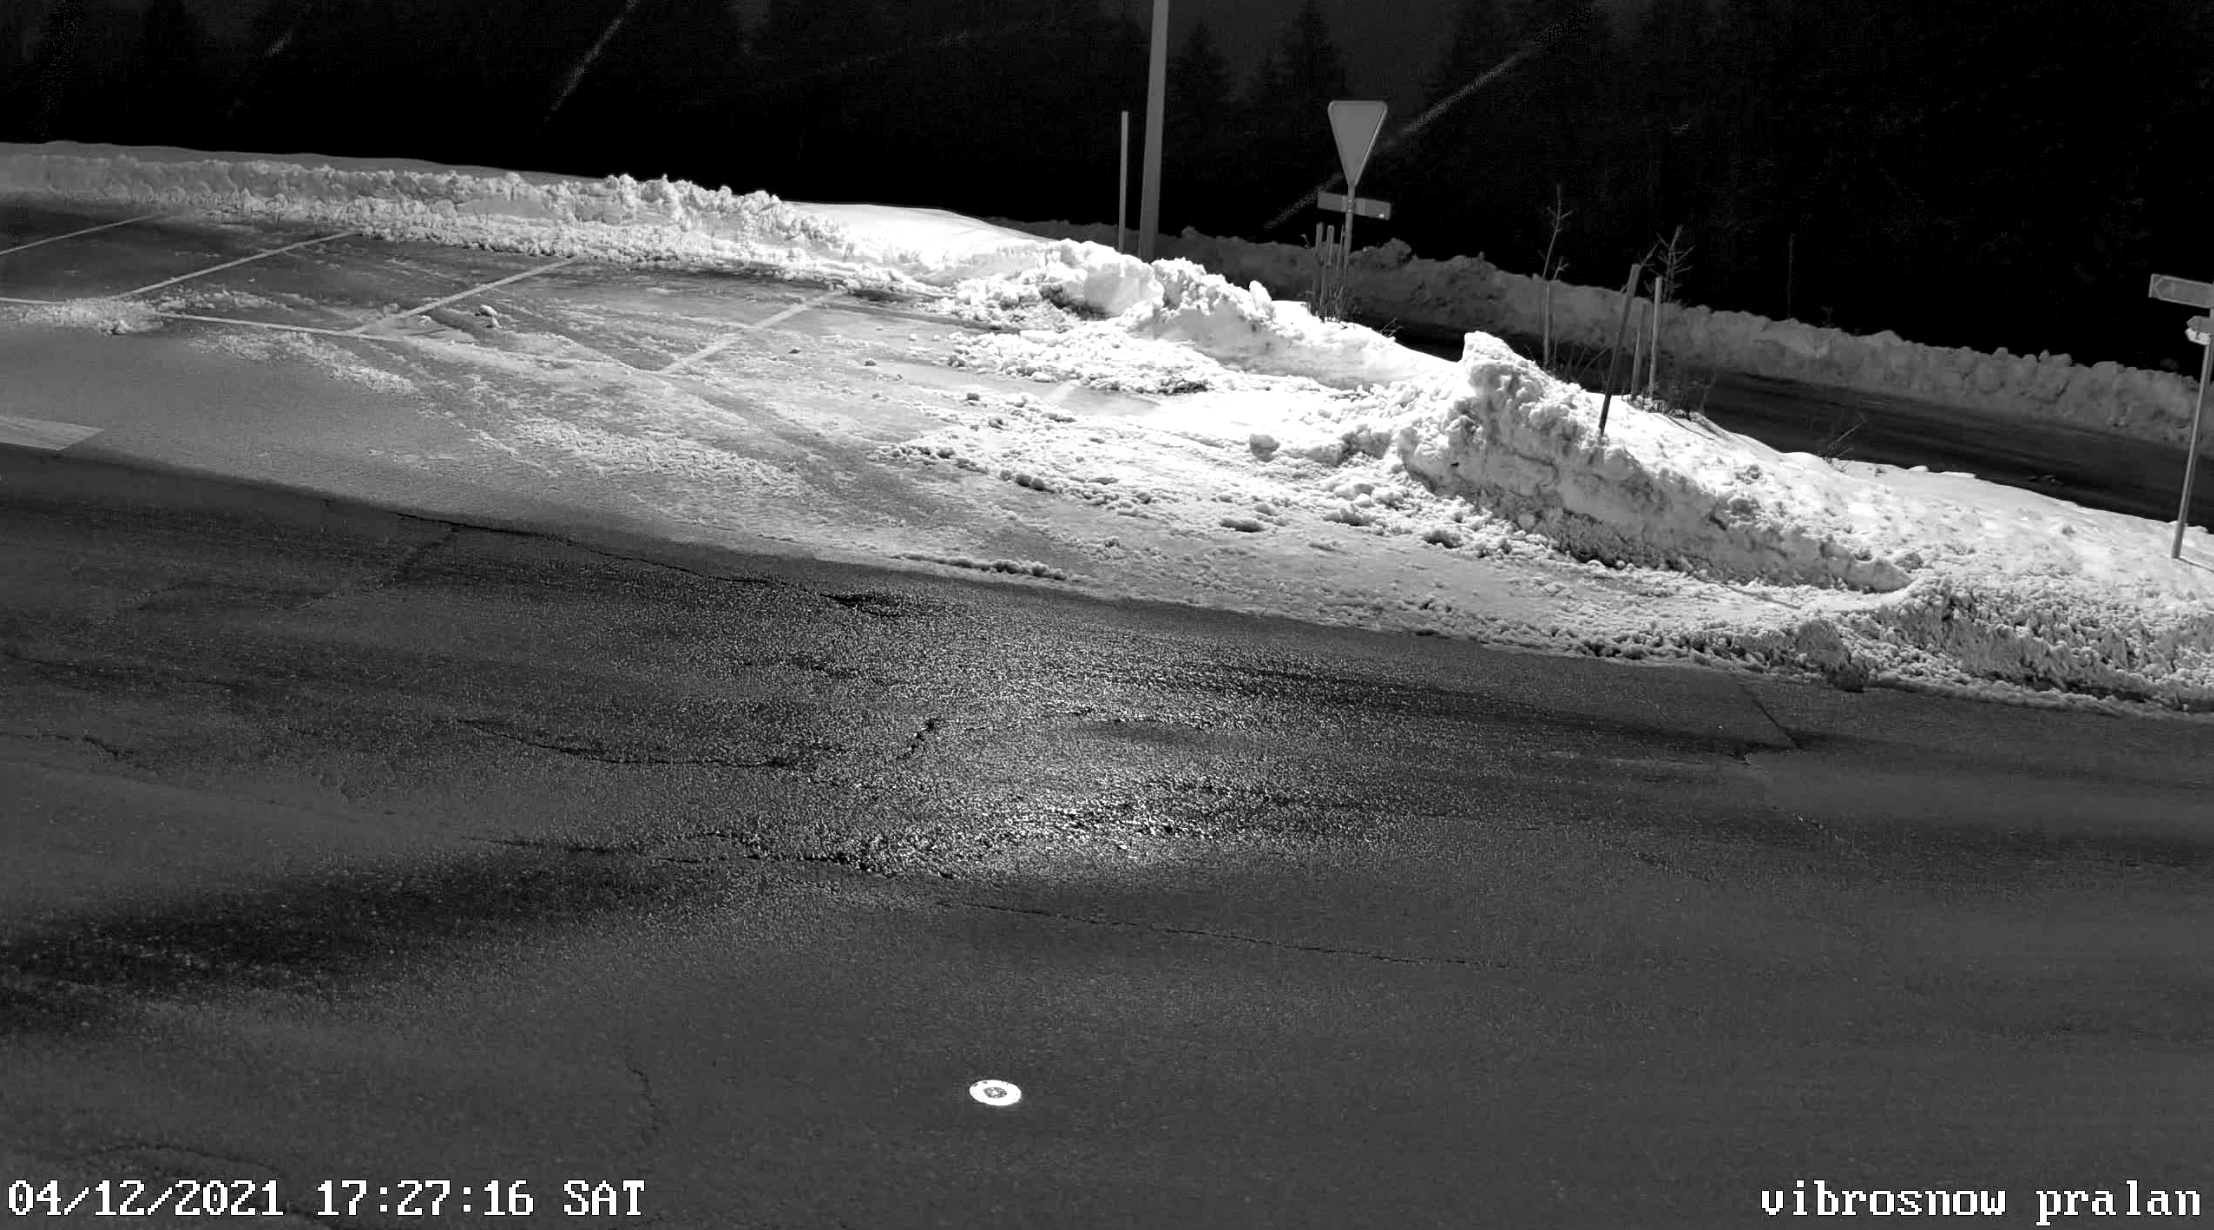
\includegraphics[width=\linewidth]{Images/computer_vision/snowOnRoad/ref_original.png}
        \caption{Image de référence originale}
        \label{fig:SnowOnRoad_ref_original}
    \end{subfigure}
    \hfill
    \begin{subfigure}{.45\textwidth}
        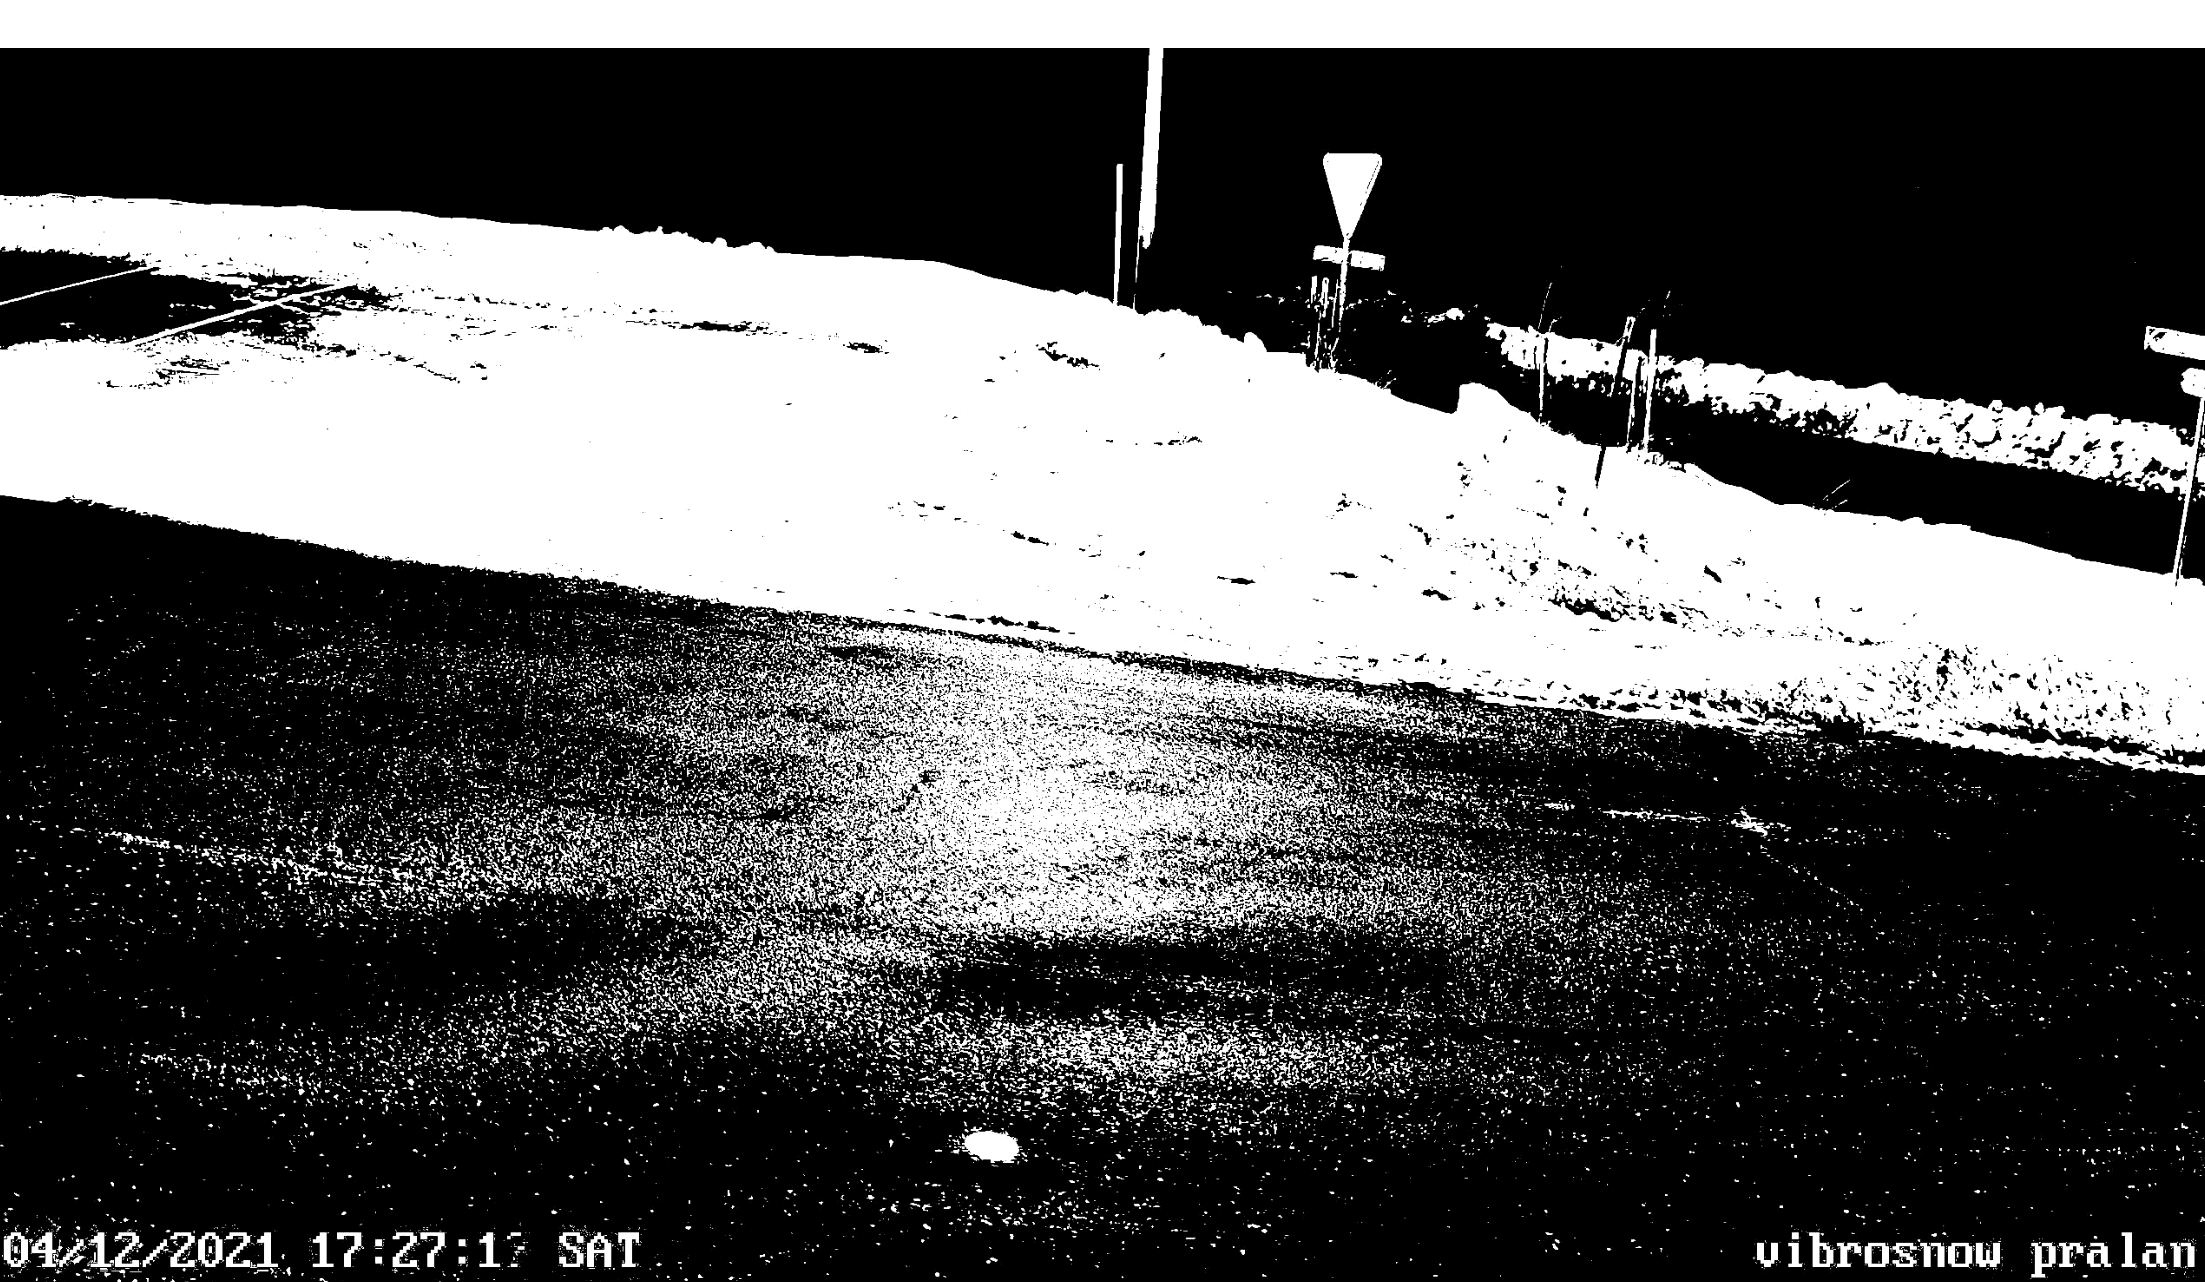
\includegraphics[width=\linewidth]{Images/computer_vision/snowOnRoad/ref_thres.png}
        \caption{Image de référence seuillée}
        \label{fig:SnowOnRoad_ref_thres}
    \end{subfigure}
    \caption{Image de référence}
    \label{fig:SnowOnRoad_ref}
\end{figure}

\begin{figure}[H]
    \begin{subfigure}{.45\textwidth}
        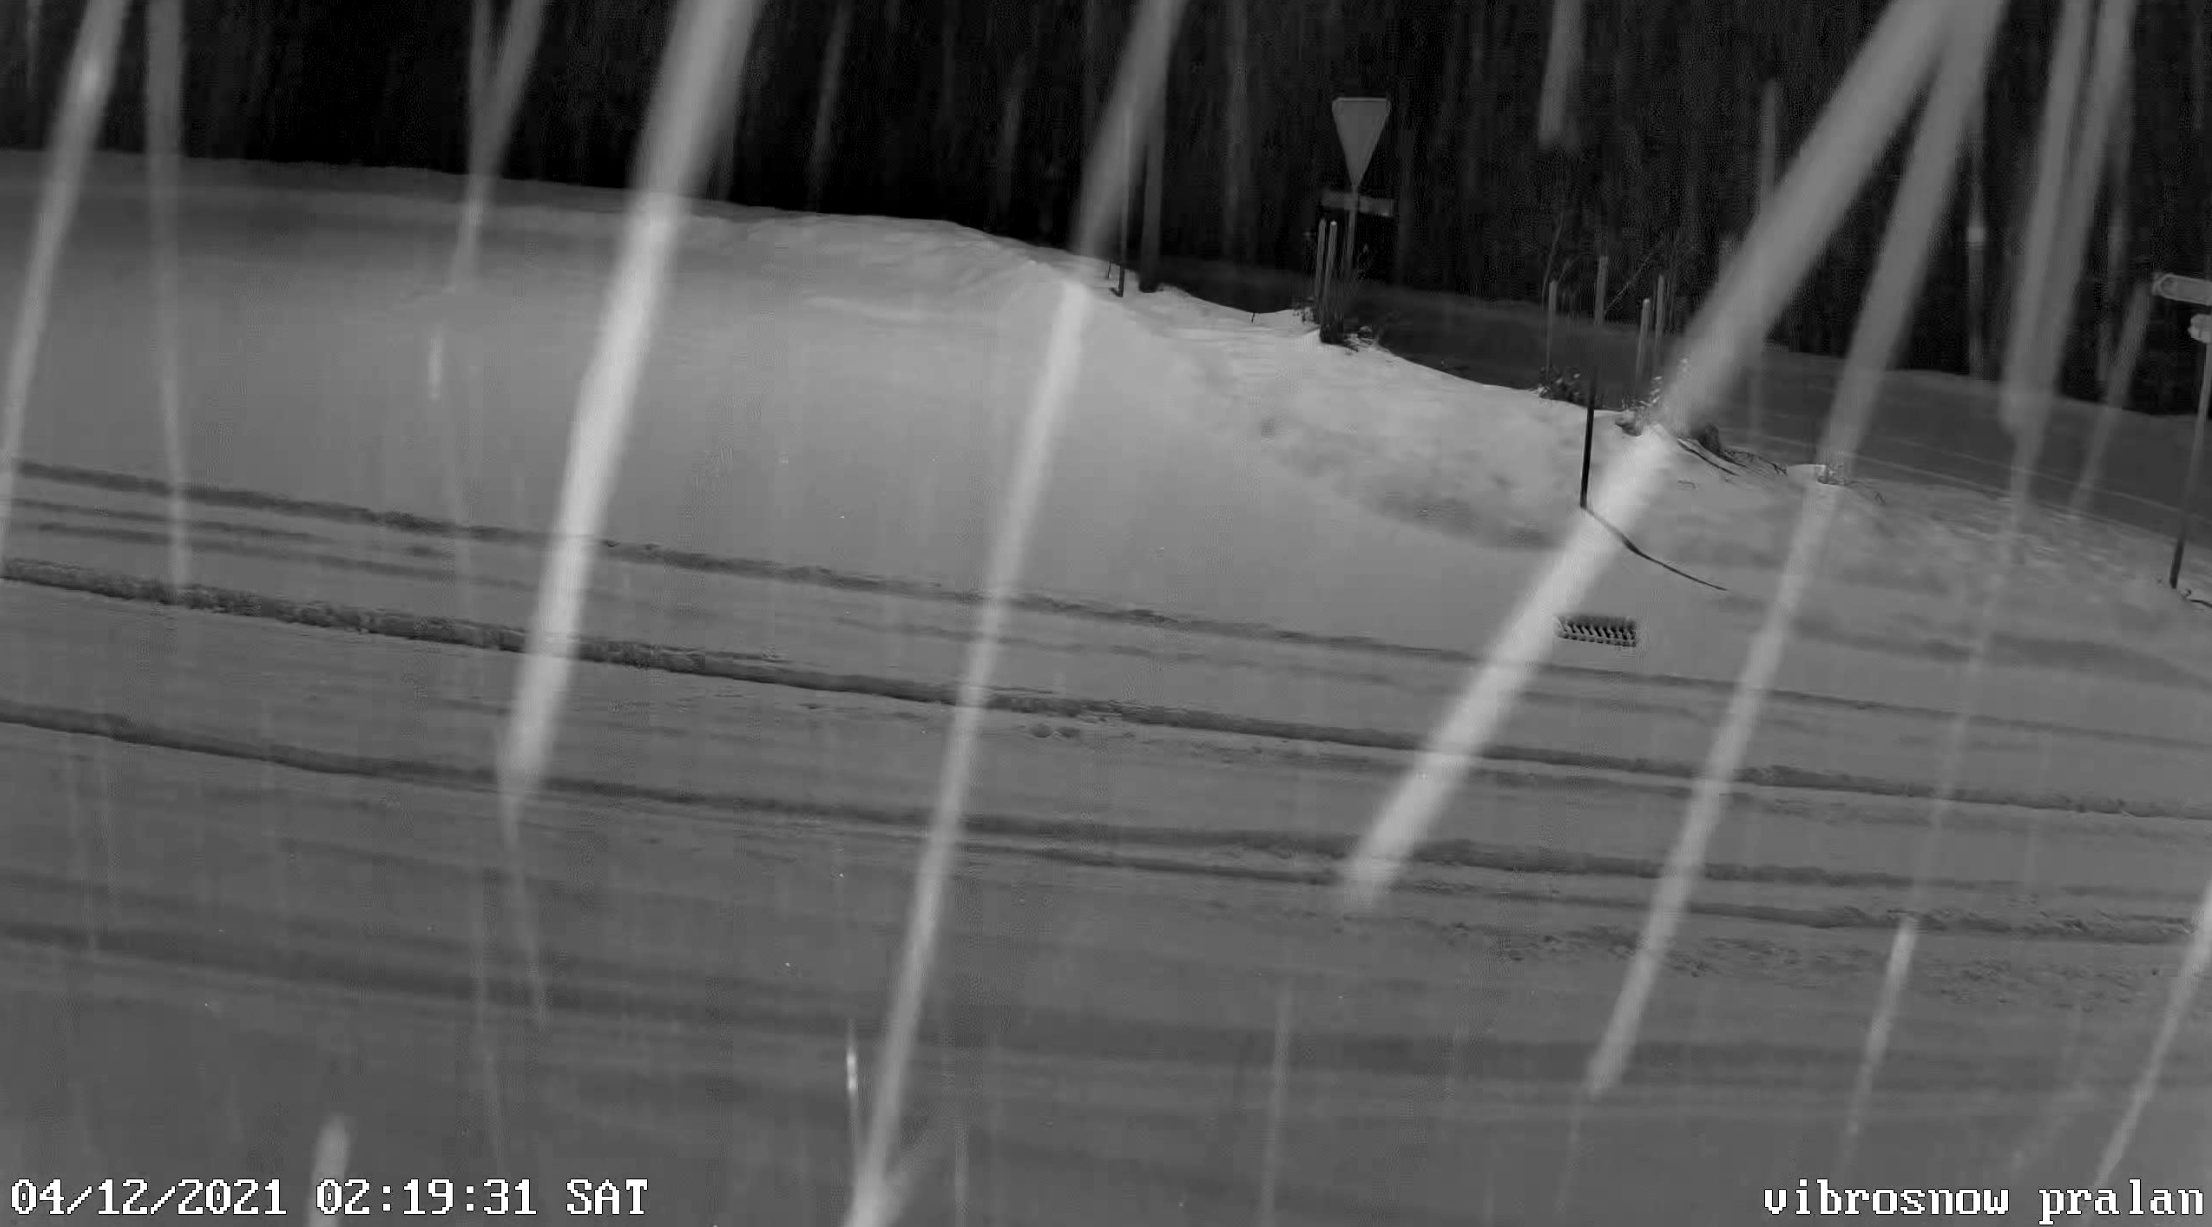
\includegraphics[width=\linewidth]{Images/computer_vision/snowOnRoad/test_original.png}
        \caption{Image de test originale}
        \label{fig:SnowOnRoad_test_original}
    \end{subfigure}
    \hfill
    \begin{subfigure}{.45\textwidth}
        
\includegraphics[width=\linewidth]{Images/computer_vision/snowOnRoad/test_thres.png}
        \caption{Image de test seuillée}
        \label{fig:SnowOnRoad_test_thres}
    \end{subfigure}
    \hfill
    \begin{subfigure}{.45\textwidth}
        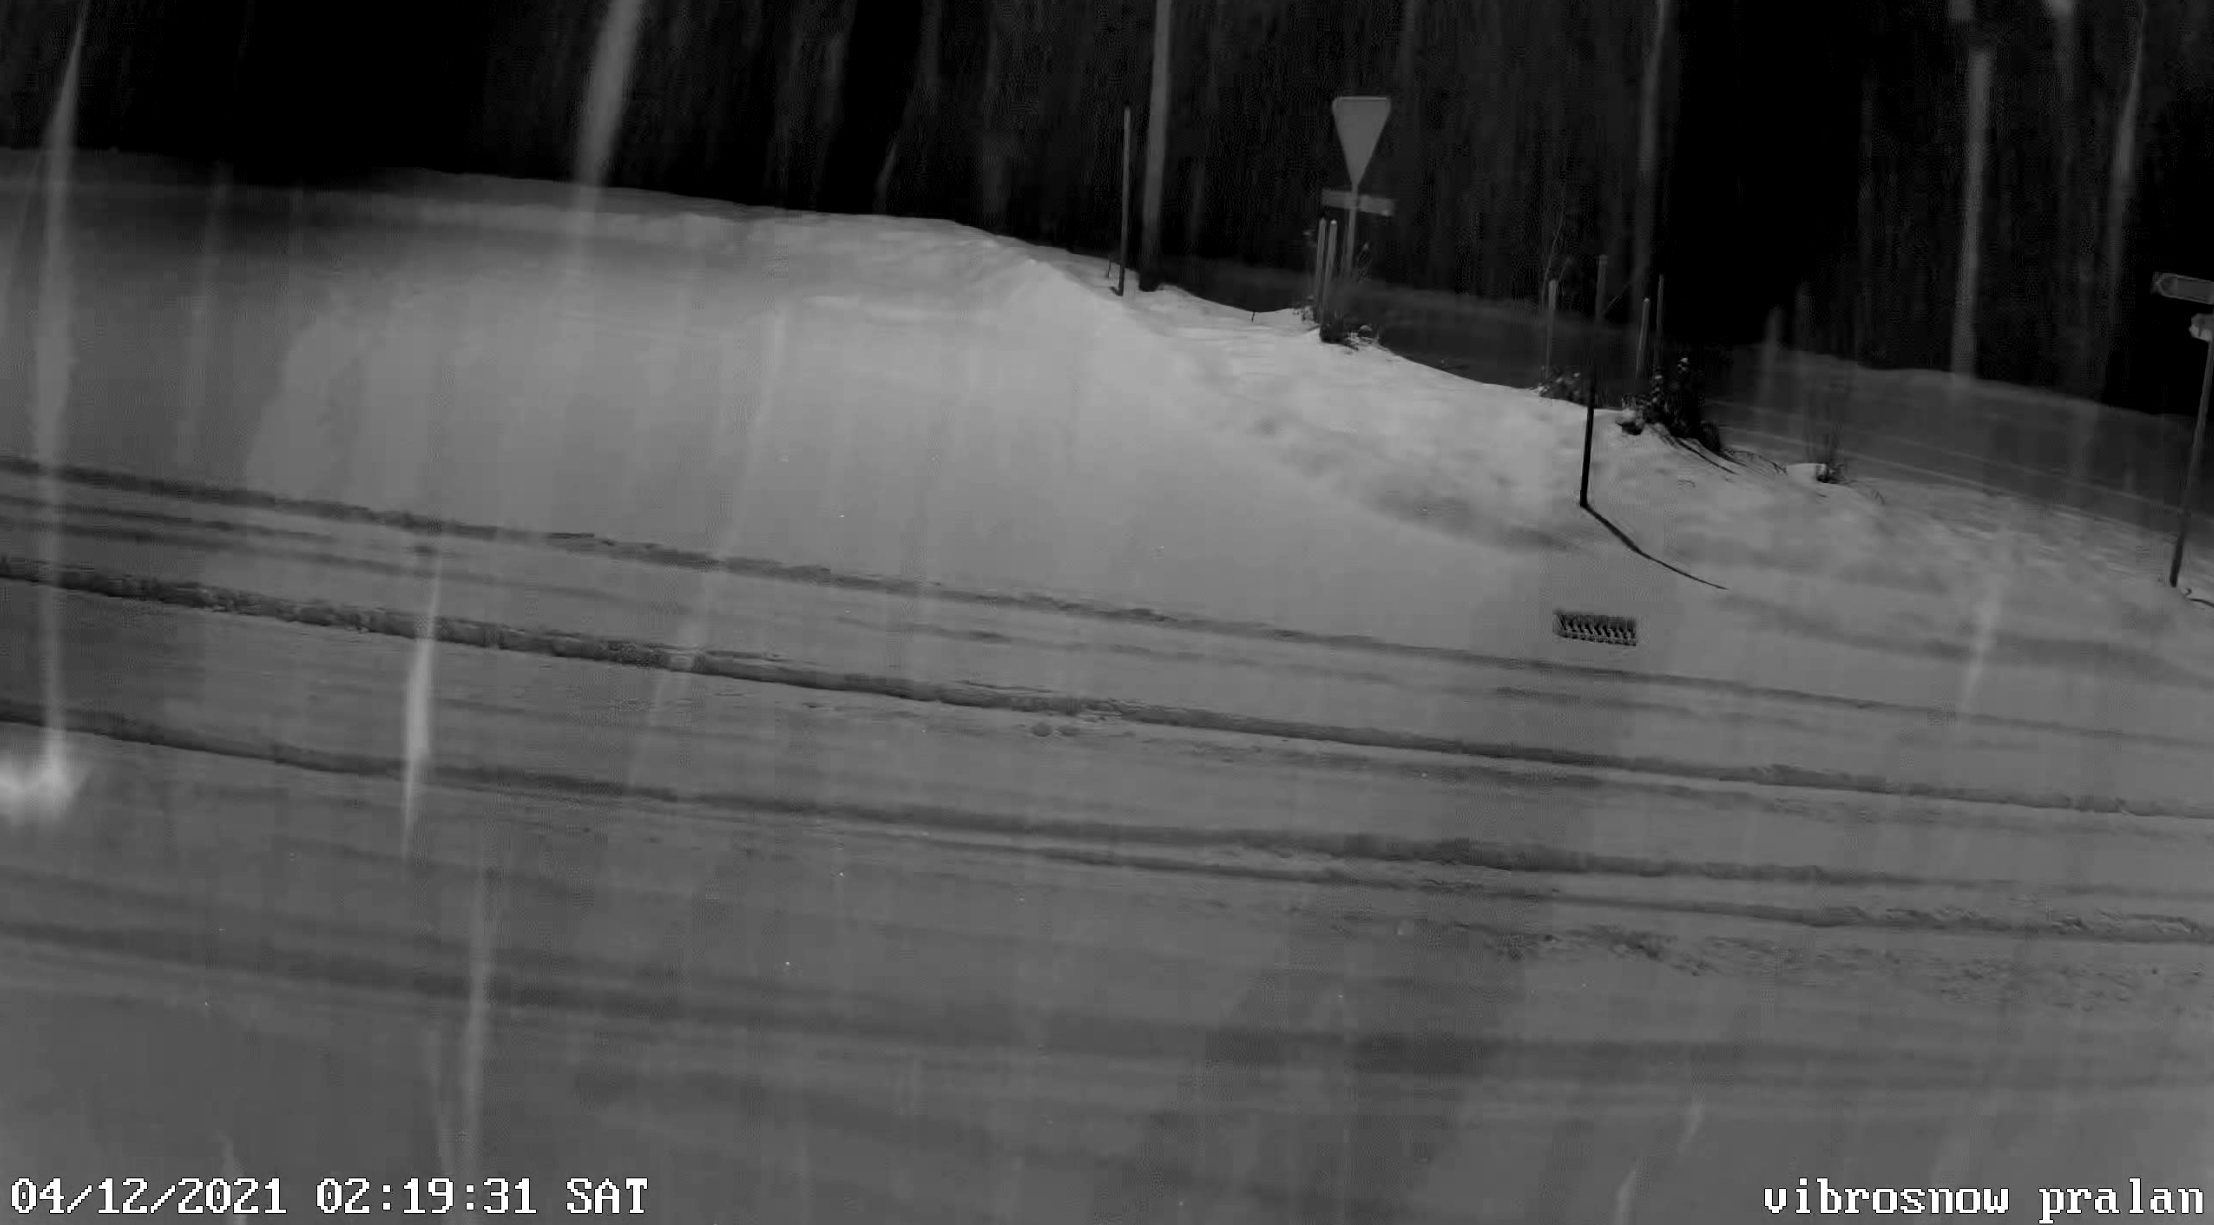
\includegraphics[width=\linewidth]{Images/computer_vision/snowOnRoad/test_denoised.png}
        \caption{Image de test avec suppression de bruit}
        \label{fig:SnowOnRoad_test_denoised}
    \end{subfigure}
    \hfill
    \begin{subfigure}{.45\textwidth}
        
\includegraphics[width=\linewidth]{Images/computer_vision/snowOnRoad/test_denoisedThres.png}
        \caption{Image de test avec suppression de bruit et seuillée}
        \label{fig:SnowOnRoad_test_denoisedThres}
    \end{subfigure}
    \caption{Image de test}
    \label{fig:SnowOnRoad_test}
\end{figure}
\newpage
\section{Résultats}

Ici seront présentés les résultats des tests qui concernent le LiDAR Lite V4. Au fur et à mesure des
résultats, quelques conclusions seront d'ores et déjà tirées.\\
En annexe, se trouve le protocole de test complet du capteur.

\subsection{Caractéristique de l'erreur de mesure}

Le premier test consiste à mesurer une distance connue avec le capteur et de noter sa valeur mesurée
afin de vérifier si la plage de mesure donnée par la fiche technique (5cm à 10m) est vraie.\\
Ceci nous permet de savoir dans quelle mesure la distance fournie par le capteur représente la réalité.
Dans le cas d'une erreur de mesure, il nous est aussi utile de savoir si cette erreur est constante 
entre plusieurs séries espacées dans le temps.

\subsubsection{Méthode}

Pour ce faire, le capteur a été placé le long d'un étalon gradué de 6 mètres. Un objet est ensuite
placé à un interval de 20cm pour le premier mètre, puis à un interval de 50cm. À chaque mesure, on 
note la valeur mesurée par le LiDAR ainsi que la distance réelle.\\
Cela nous permet donc de comparer la plage de mesure effective du capteur, dans les tolérences
annoncées. La figure \ref{fig:RealDistanceMeasures} montre la mise en place du test de distance.

\begin{figure}[H]
    \centering
    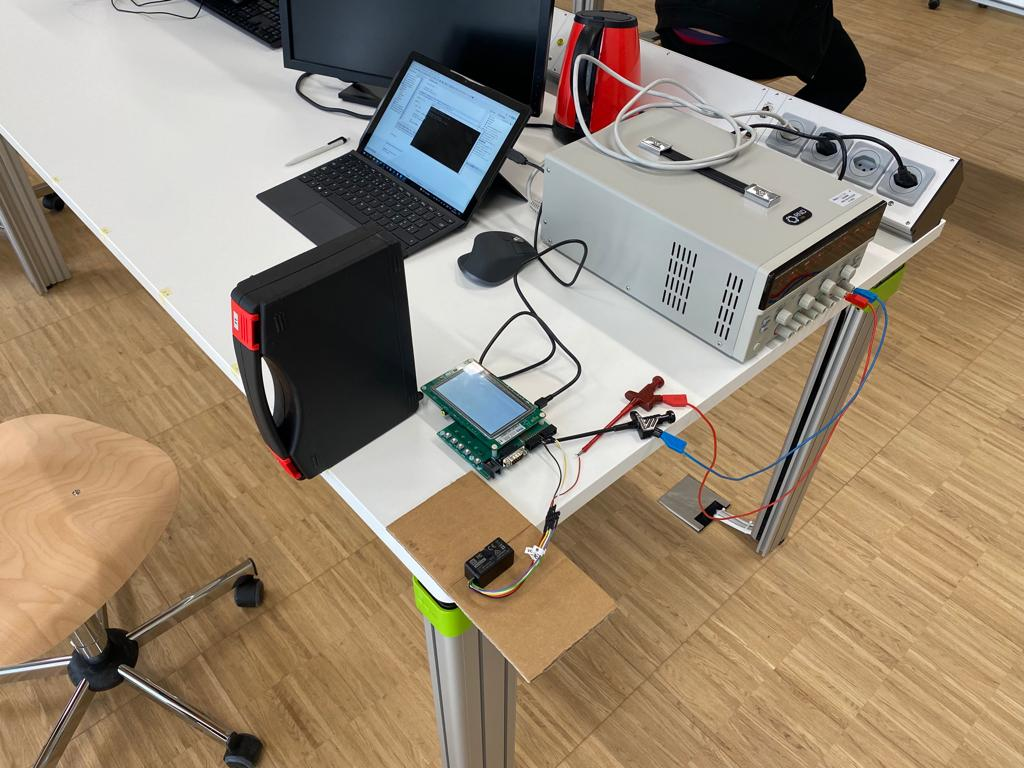
\includegraphics[width=0.5\textwidth]{Images/LiDAR/RealDistanceMes.jpeg}
    \caption{Mesure de distance comparée à la distance réelle}
    \label{fig:RealDistanceMeasures}
\end{figure}

La mesure finale de distance est une moyenne de 10 mesures. Cela permet notamment d'éliminer partiellement
l'erreur due à la résolution finie du capteur.\\
Le test a été réalisé en intérieur, en l'absence total d'élément perturbateur, notamment de rayons 
infrarouges, à température ambiante (25°C).

\subsubsection{Résultats du test}

\begin{figure}[H]
    \centering
    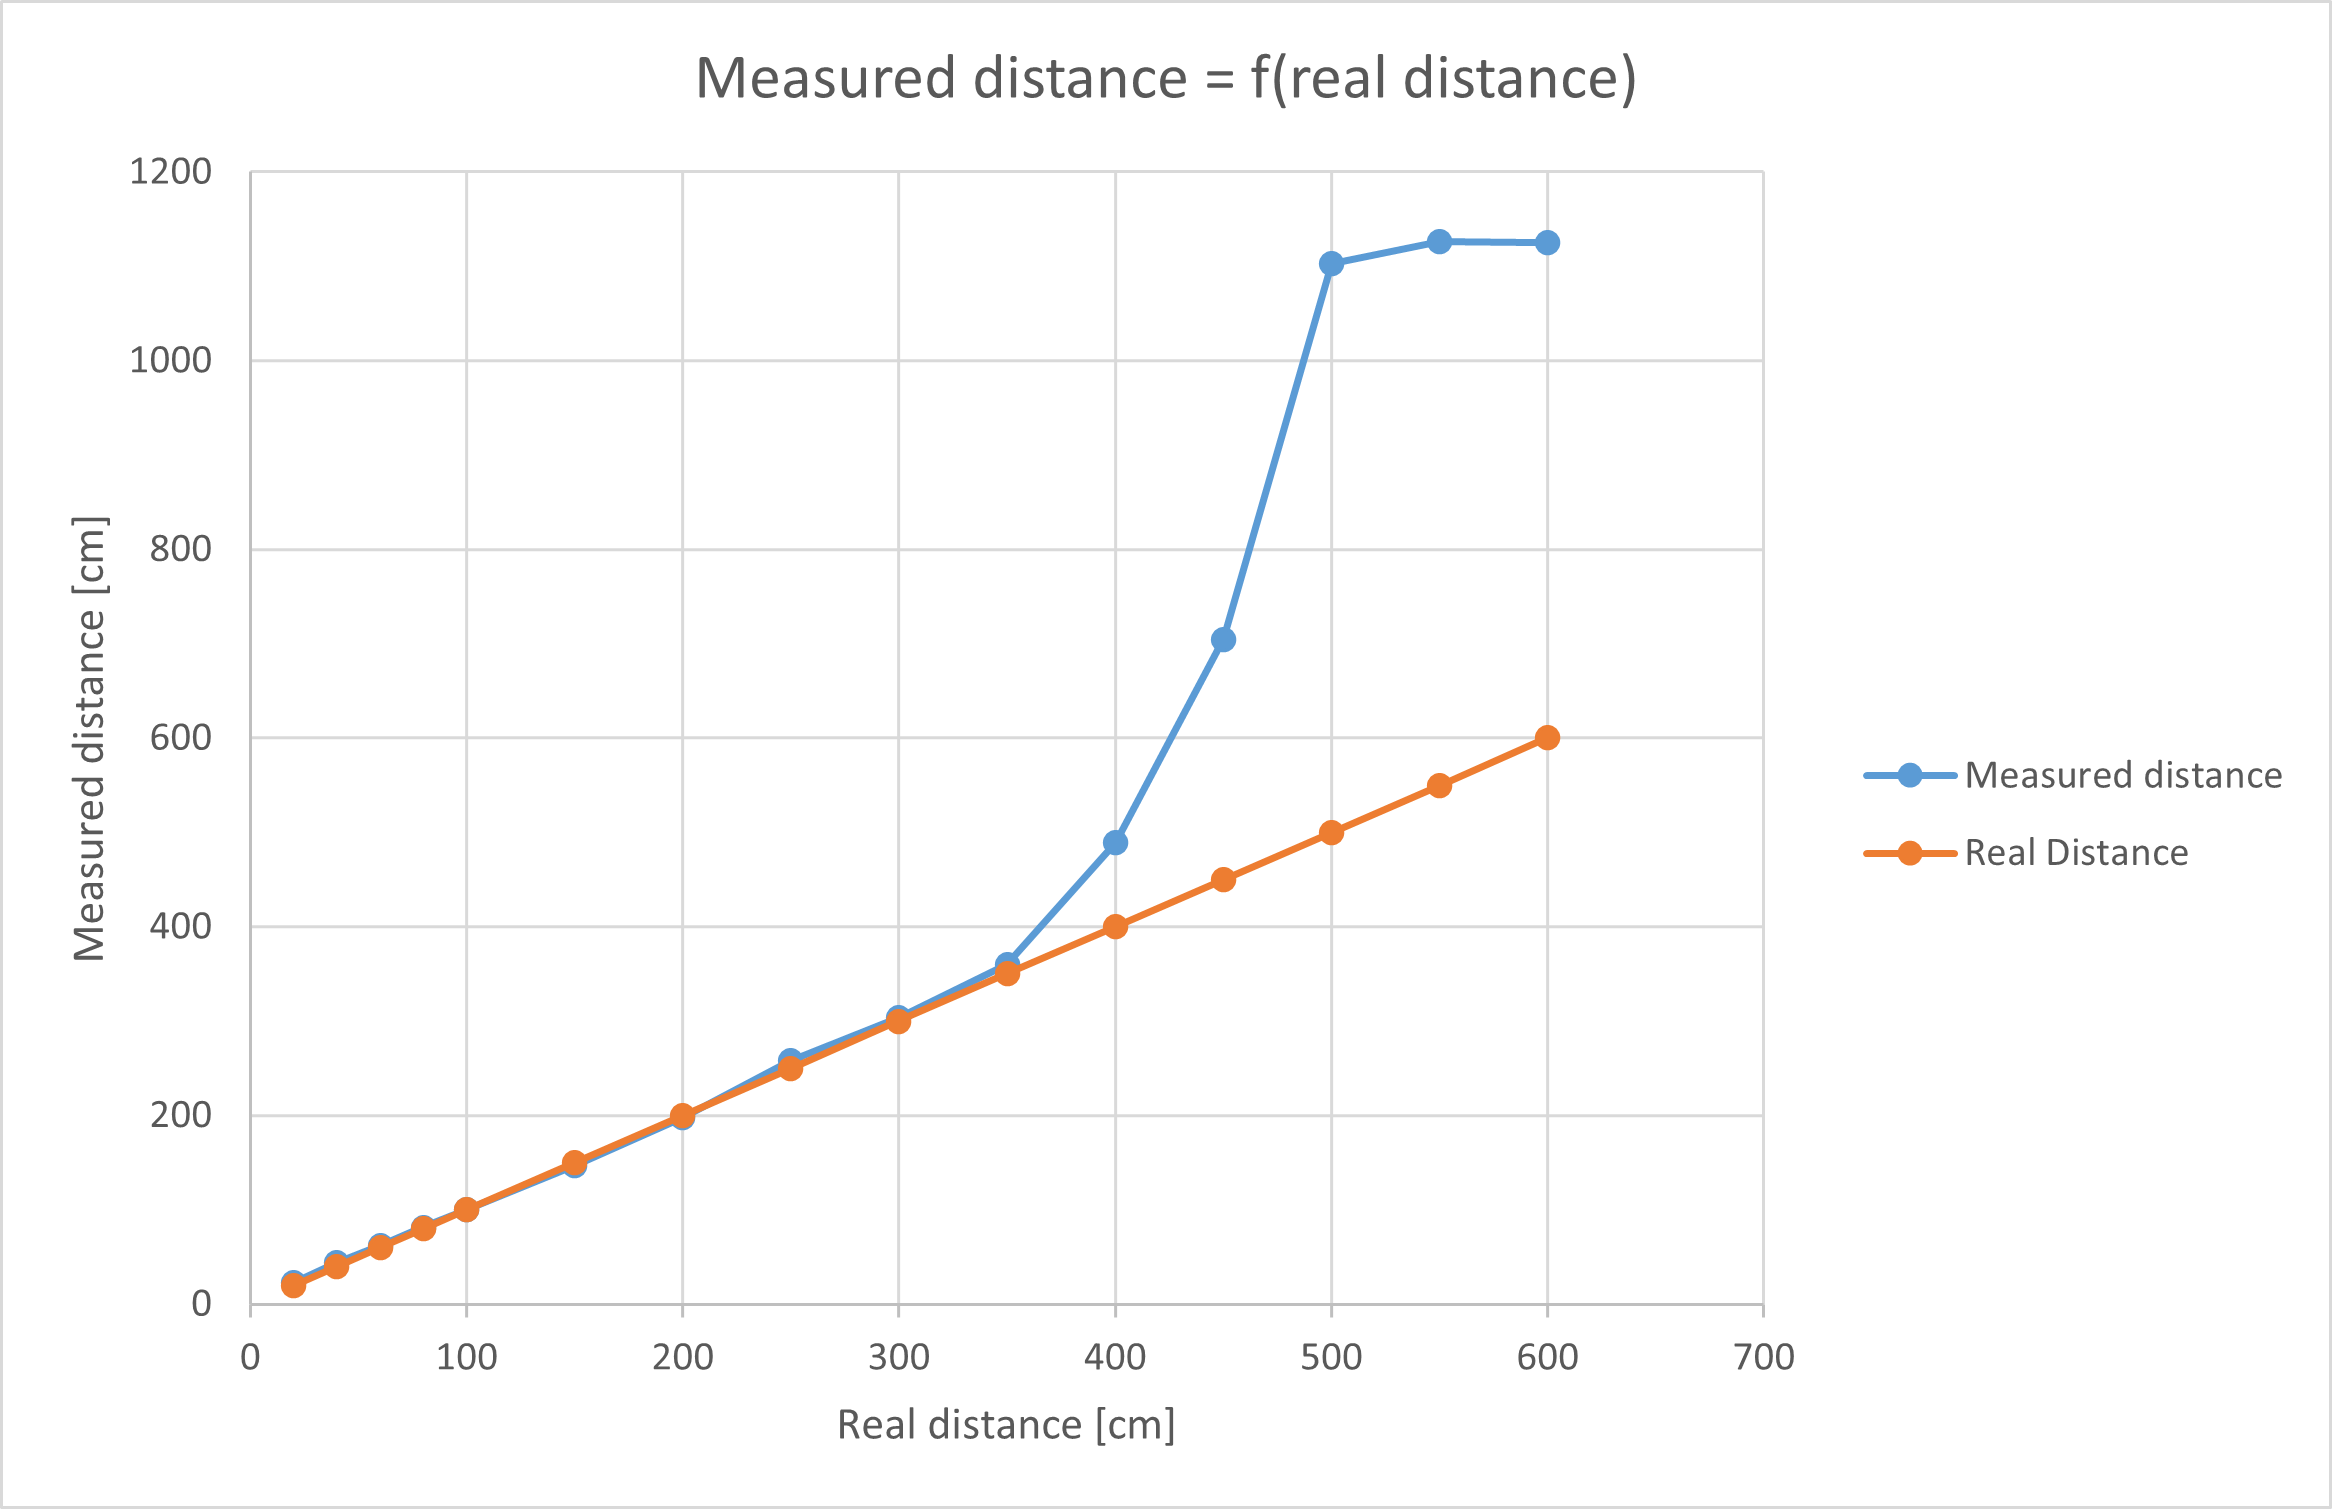
\includegraphics[width=0.8\textwidth]{Images/LiDAR/LiDARRealDistanceGraph_MesDist.png}
    \caption{Distance mesurée en fonction de la distance réelle}
    \label{fig:RealDistanceMesGraph}
\end{figure}

\begin{figure}[H]
    \centering
    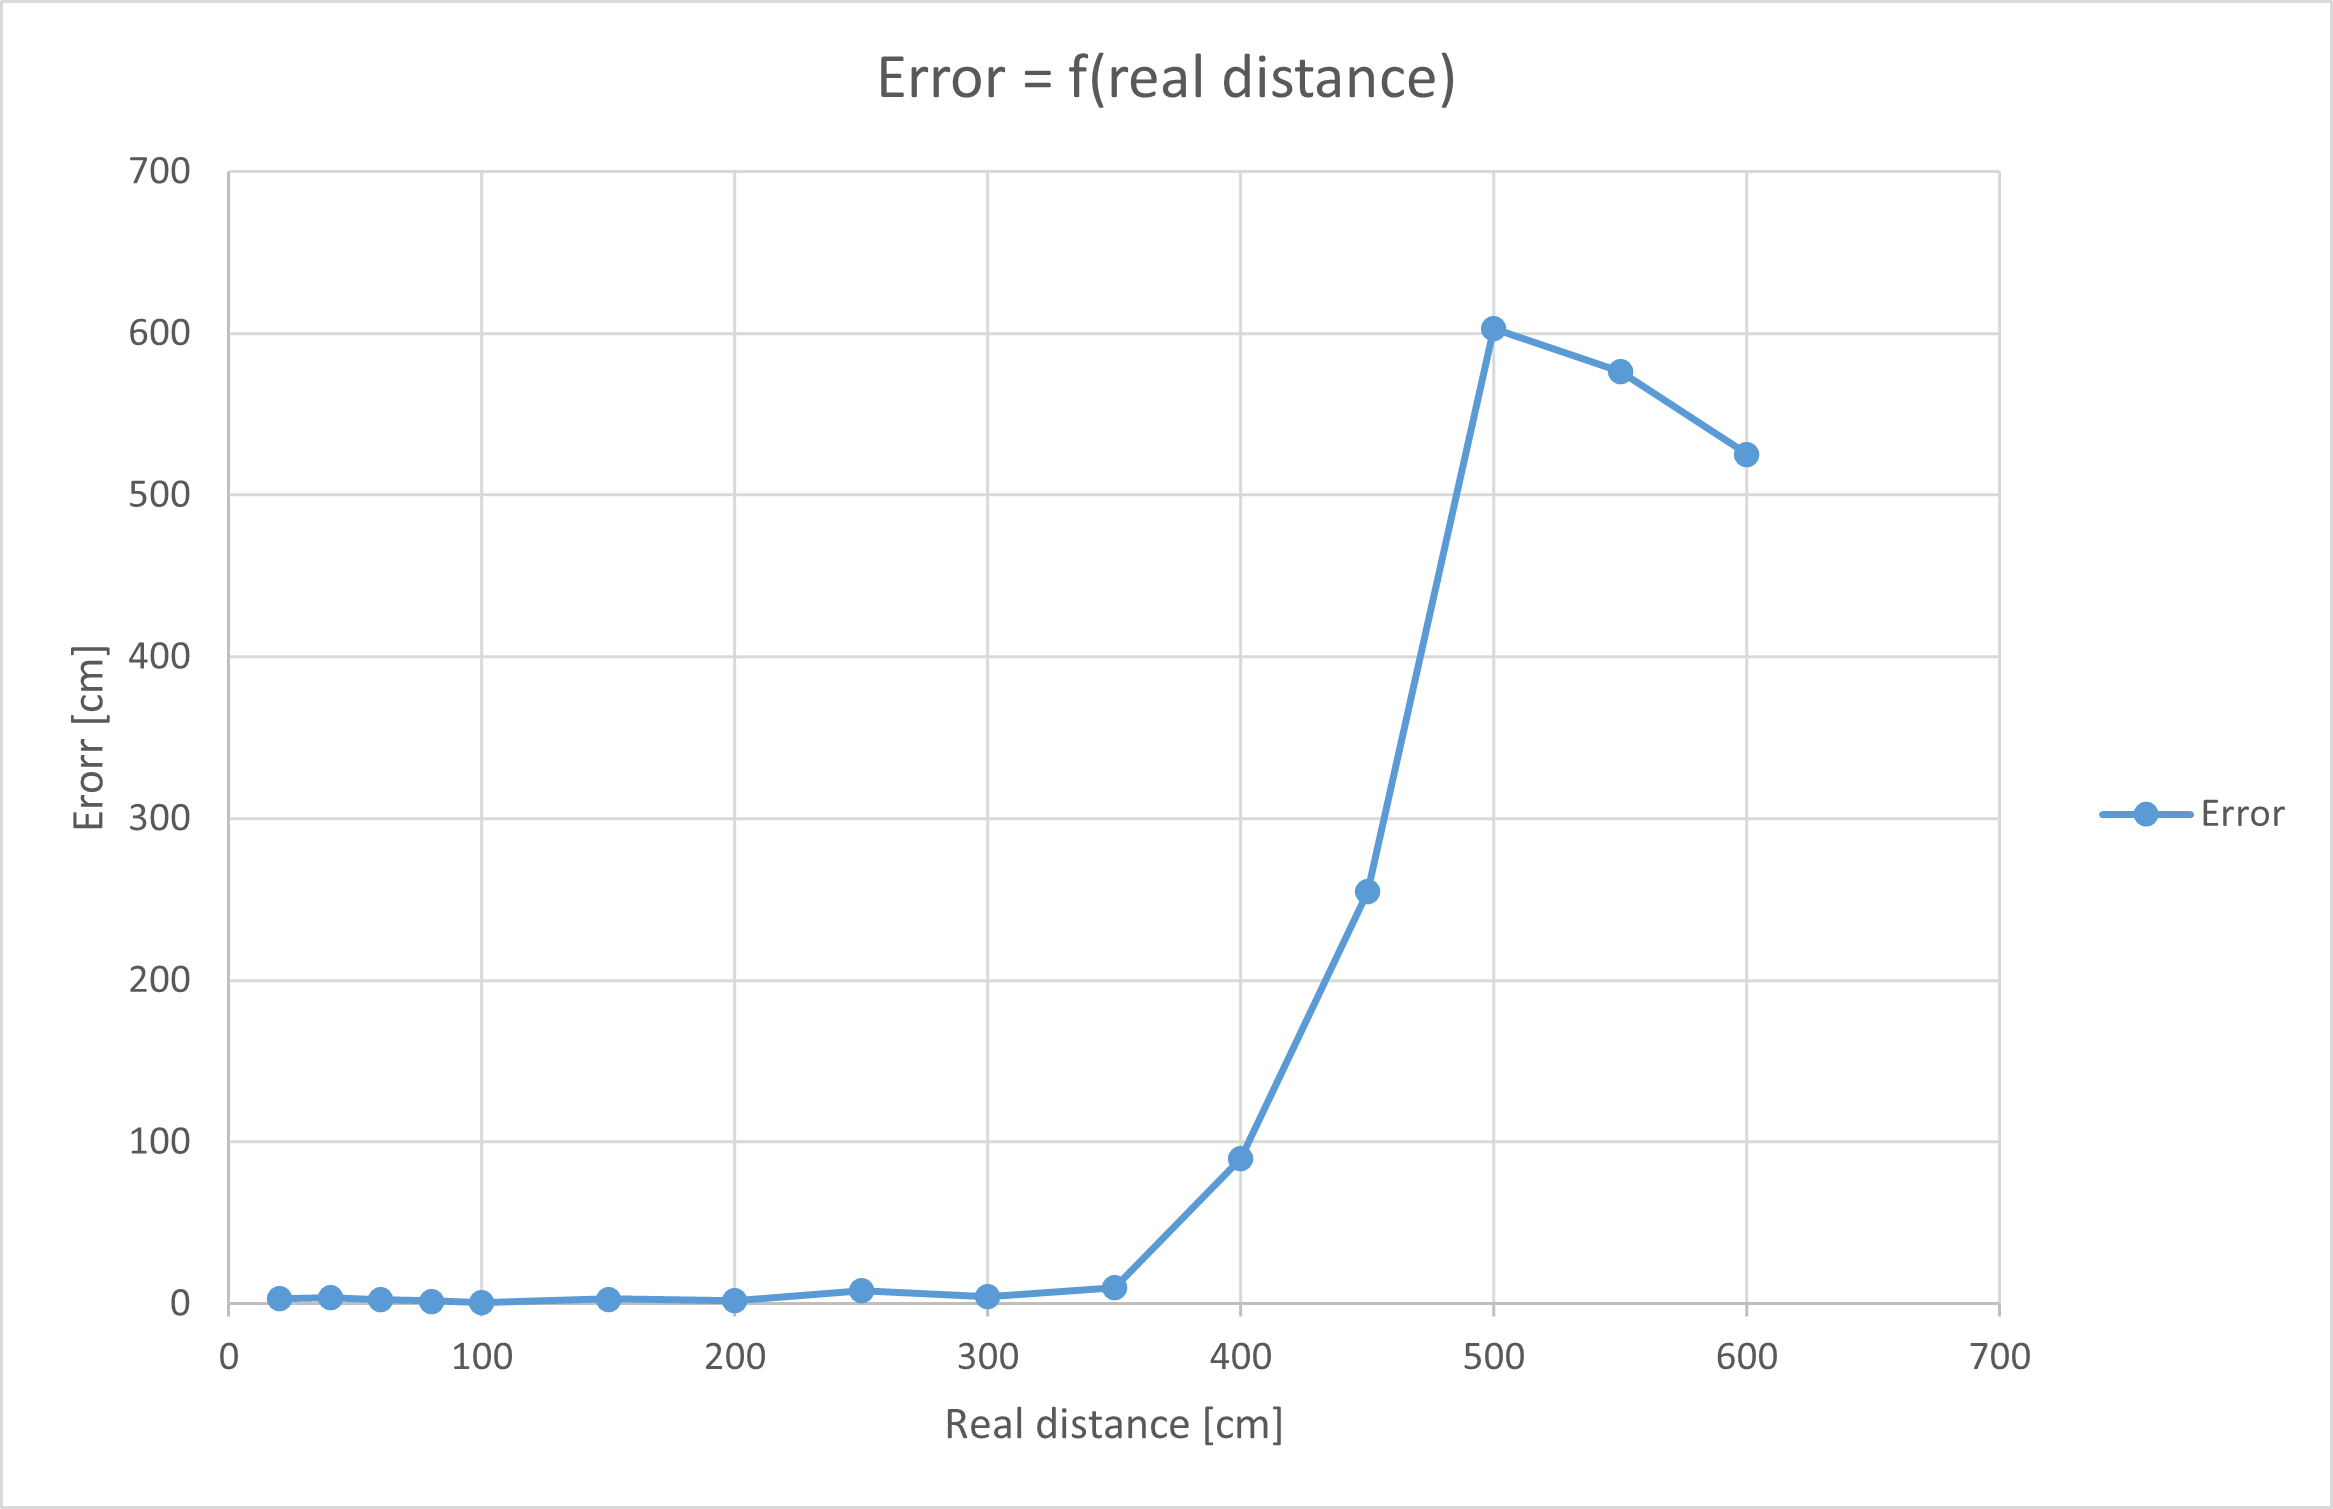
\includegraphics[width=0.8\textwidth]{Images/LiDAR/LiDARRealDistanceGraph_MesDistError.png}
    \caption{Erreur de la distance mesurée par rapport à la distance réelle}
    \label{fig:RealDistanceMesGraphError}
\end{figure}

Nous avons jugé important de zoomer sur la plage utile entre 0 et 3m afin de visualiser les graphes 
de manière plus claire.

\begin{figure}[H]
    \centering
    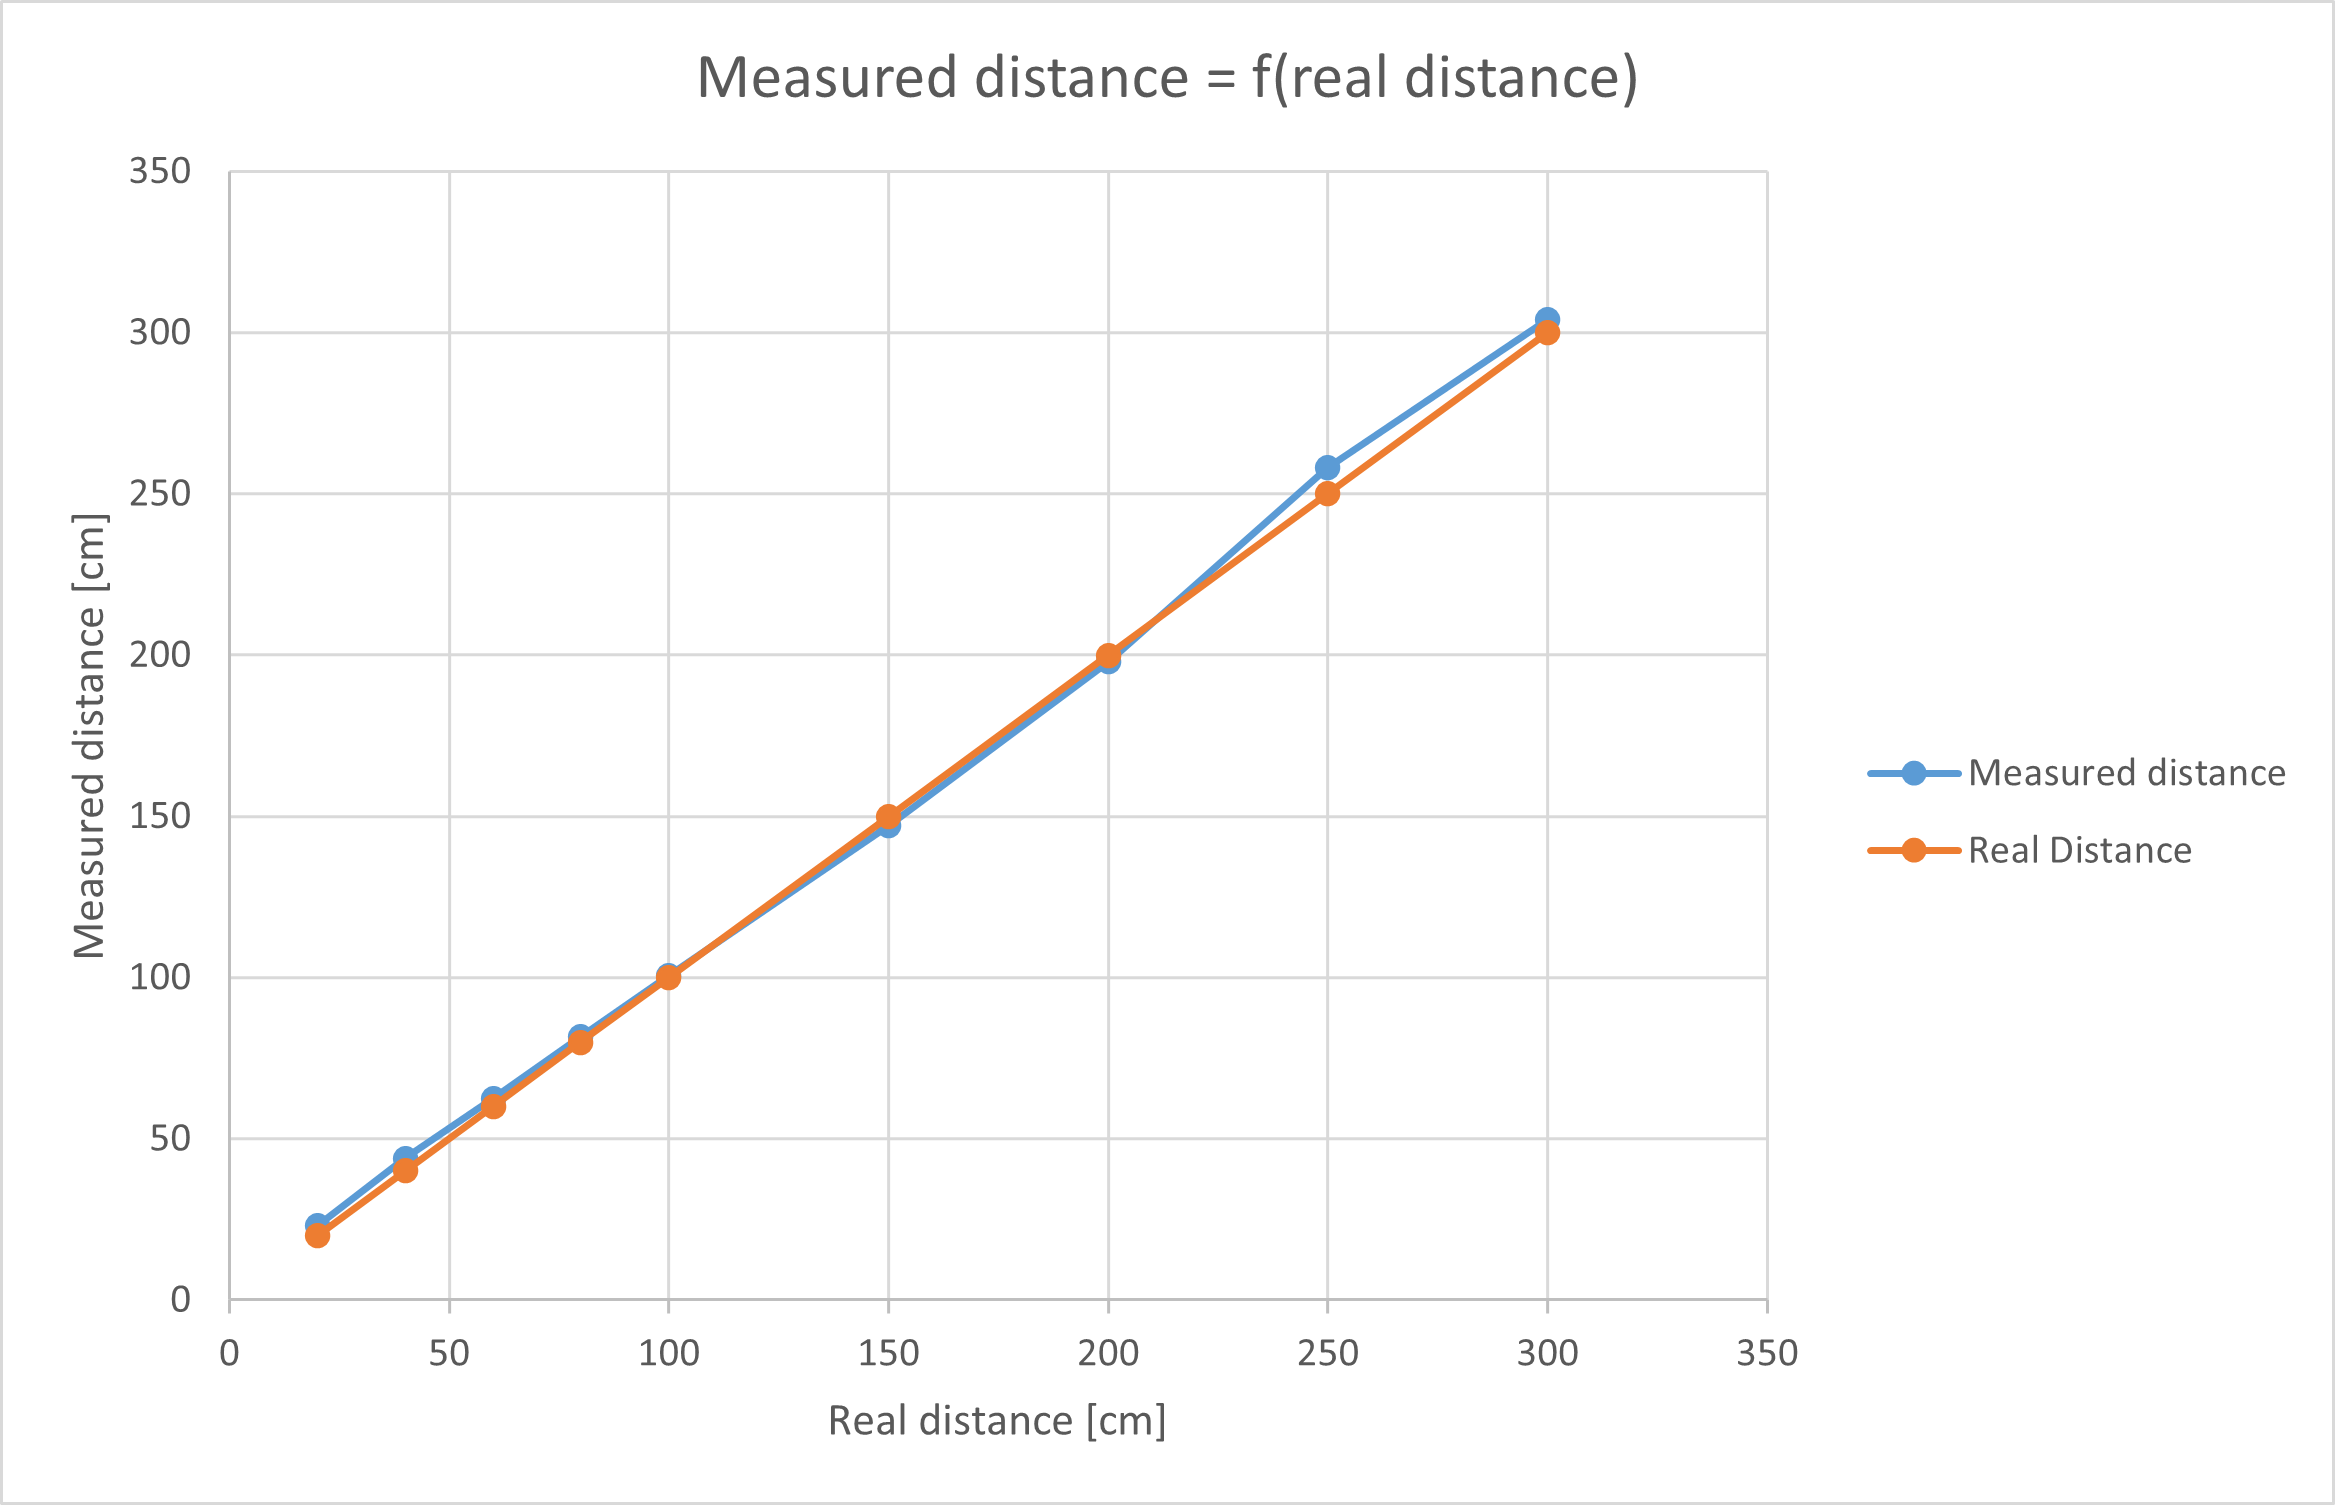
\includegraphics[width=0.8\textwidth]{Images/LiDAR/LiDARRealDistanceGraph_MesDist_Zoom.png}
    \caption{Distance mesurée en fonction de la distance réelle dans la plage utile}
    \label{fig:RealDistanceMesGraphZoom}
\end{figure}

\begin{figure}[H]
    \centering
    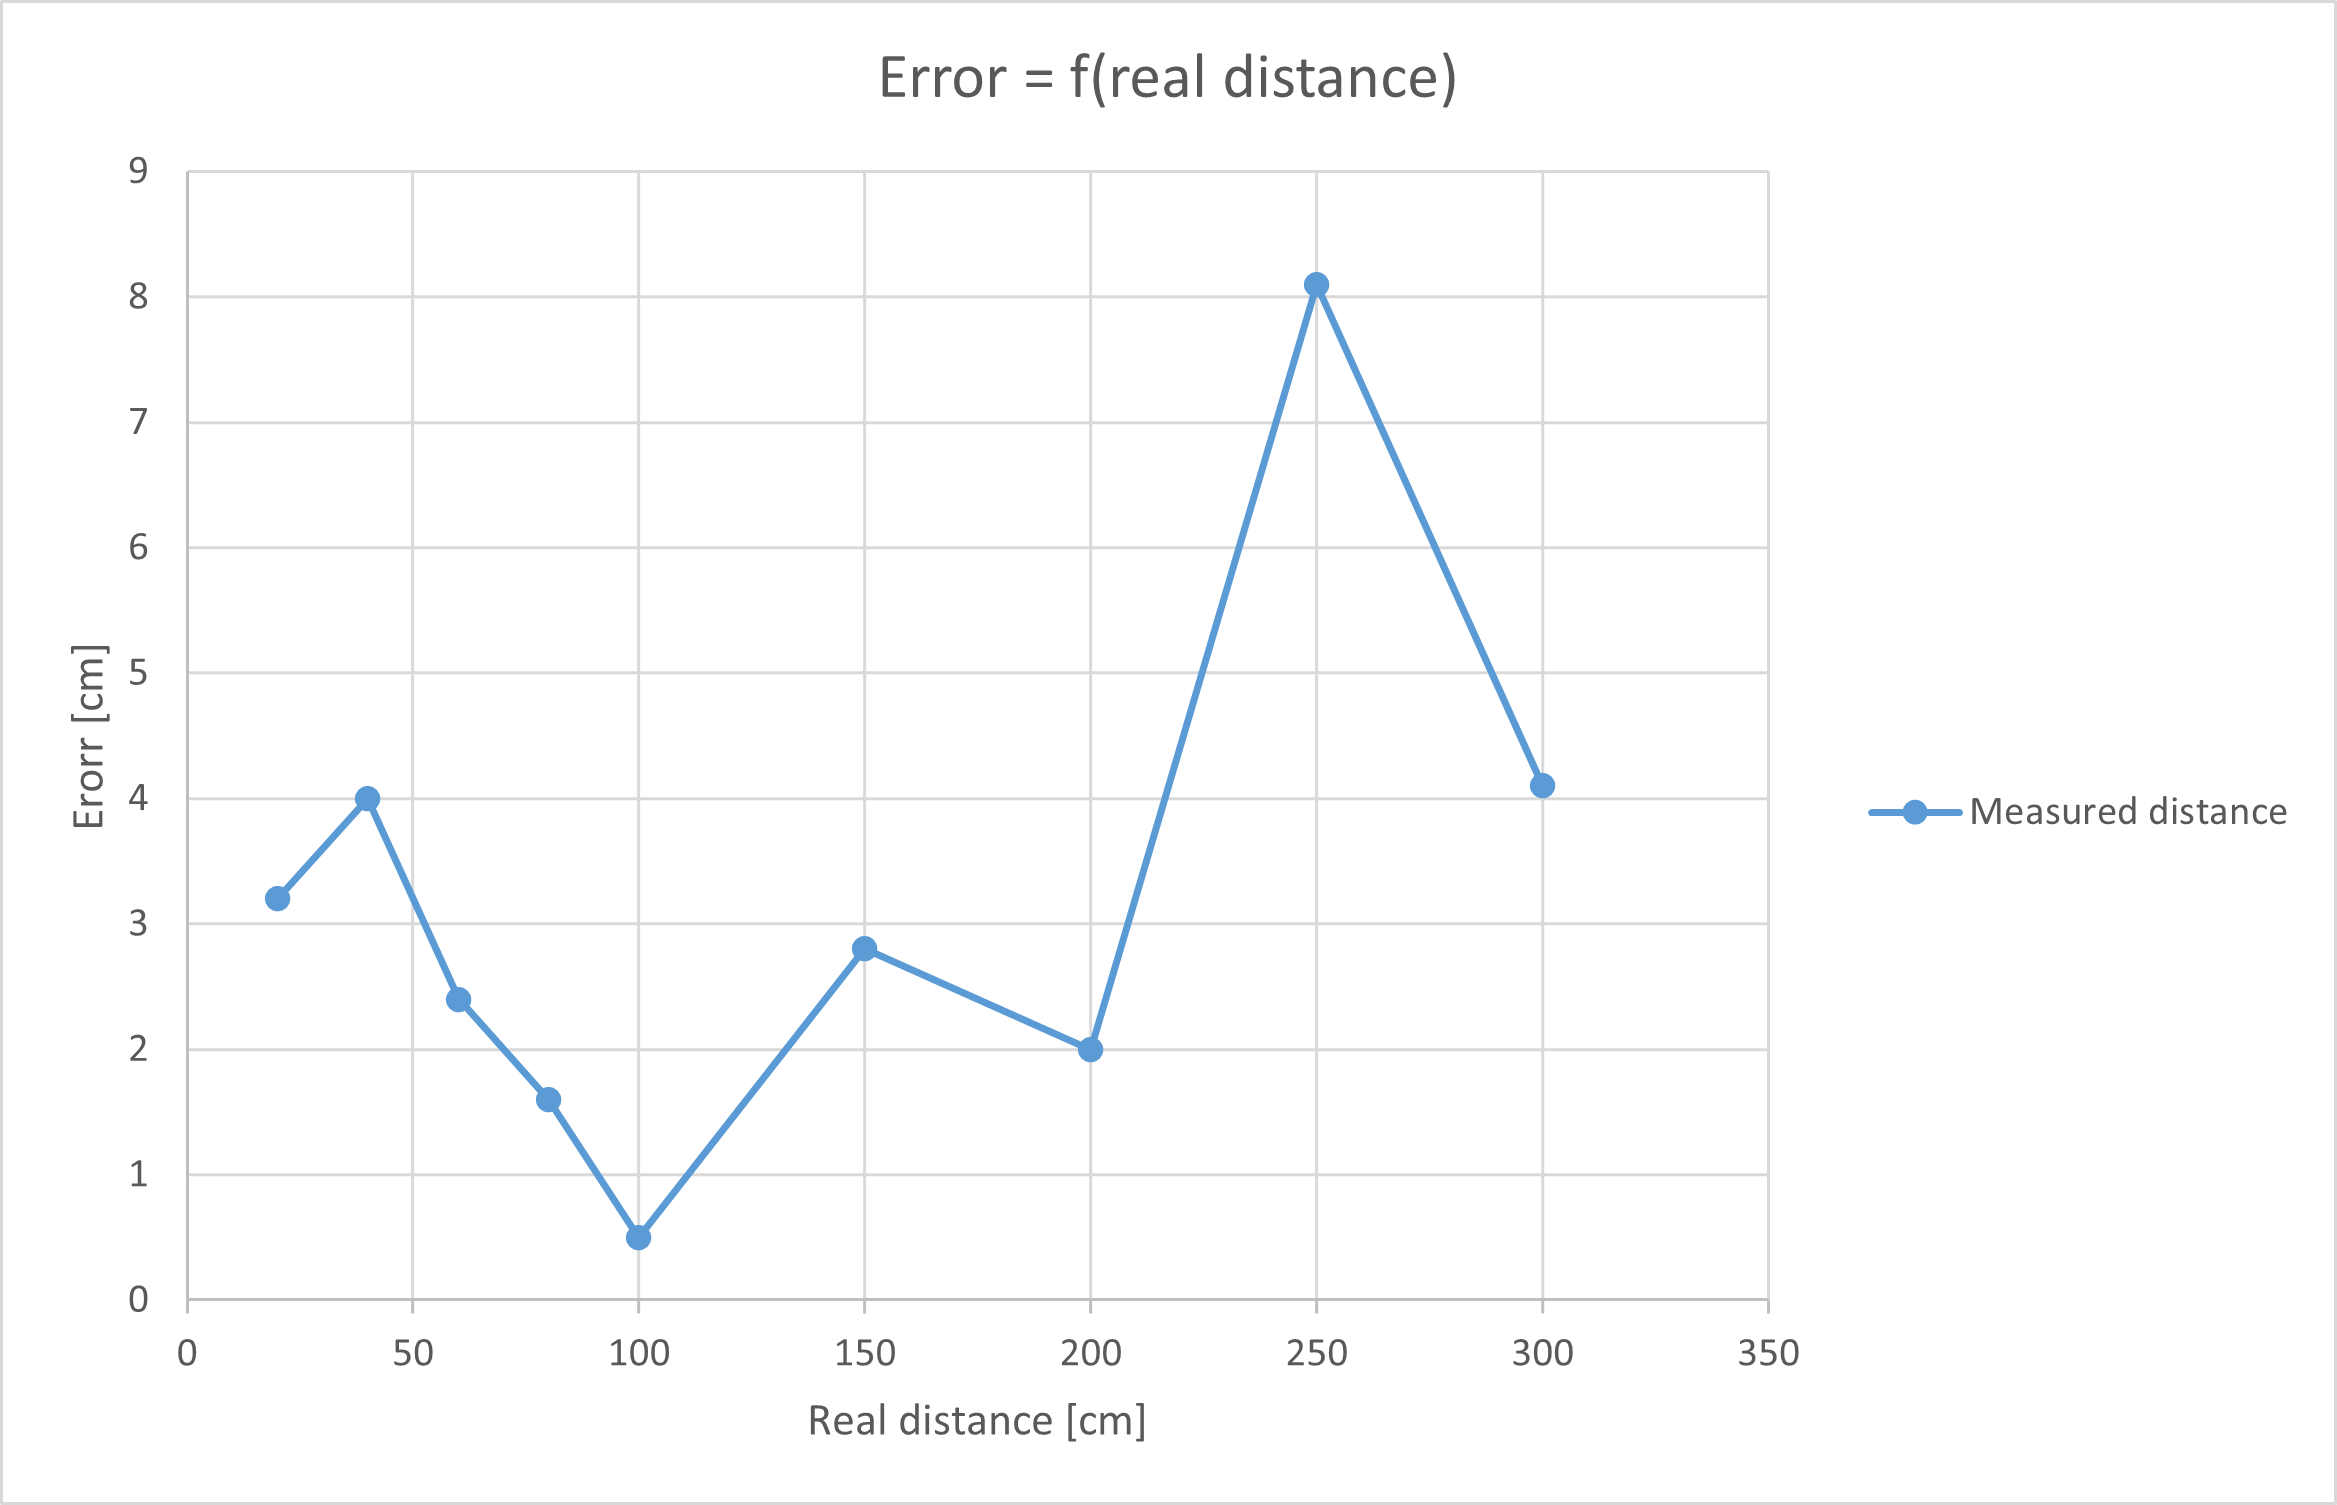
\includegraphics[width=0.8\textwidth]{Images/LiDAR/LiDARRealDistanceGraph_MesDistError_Zoom.png}
    \caption{Erreur de la distance mesurée par rapport à la distance réelle dans la plage utile}
    \label{fig:RealDistanceMesGraphErrorZoom}
\end{figure}

\subsubsection{Conclusion préliminaire}

On constate très facilement sur la figure \ref{fig:RealDistanceMesGraph} que le capteur est perdu au delà
de 3.5m, soit bien moins qu'annoncé par le fabricant. La figure \ref{fig:RealDistanceMesGraphError} nous 
montre une erreur absurde de plus de 5 mètres. On conclut donc que ce capteur ne pourra pas être utilisé
pour des distances de plus de 3.5m.\\
Comme cette grande erreur aplatit totalement les mesures sous 3.5m, nous avons jugé utile d'effectuer un
zoom sur cette plage utile. On constate alors que la distance mesurée par le LiDAR reflète avec plus ou
moins de précision la distance réelle, comme le montre la figure \ref{fig:RealDistanceMesGraphZoom}.
Lorsqu'on trace l'erreur en fonction de la distance réelle, on remarque une erreur généralement bien plus
élevée qu'annoncé (figure \ref{fig:RealDistanceMesGraphErrorZoom}), soit \textpm 1cm pour des distances de 
moins de 2m et \textpm 2cm entre 2 et 4m. Cependant, il faut se rappeler que ce graphe montre uniquement 
l'erreur à la distance réelle, et non l'erreur de répétabilité. Or, comme ces mesures sont un condensé 
de plusieurs séquences espacées dans le temps, on remarque que l'erreur est constante, qui donc peut 
être compensée. De plus, dans le projet, on ne travaille qu'avec des offsets, ce qui limite d'autant 
plus les effets de cette erreur.\par

On peut finalement conclure que ce test est réussi. En effet, malgré une erreur non-négligeable de mesure,
le capteur a une répétabilité constante. Nous pouvons donc passer au test suivant.

\subsection{Mesures de distance dans un environnement perturbé}
\label{fig:MesNoise}

Maintenant que nous savons que le capteur a une répétabilité acceptable, nous cherchons à déterminer comment 
le LiDAR réagit dans un environnement perturbé. Ainsi, un banc de test a été construit afin de projeter 
des confettis devant le capteur lorsqu'il mesure. Les détails de sa construction sont expliqués dans la
section correspondante. Le but final est de générer du bruit de mesure afin de représenter au mieux une
situation réelle, par exemple en pleine tempête de neige. Nous pourrons ainsi développer une méthode
de mesure qui permet en tout temps de mesurer une hauteur de neige.

\subsubsection{Méthode}

Afin de vérifier ce test, le capteur ainsi que la plaque de développement ont été montés sur un trépied
à environ 1.5m au-dessus du sol, avec un angle de 60° par rapport à la verticale. Le LiDAR pointe le sol,
nettoyé au préalable et donc sans confetti. 100 mesures de distance sont réalisées à chaque série afin
d'avoir assez d'échantillons pour quantifier le bruit généré.\\
Sur l'appui du bouton utilisateur de la carte, le programme lance une série de 100 mesures en direction
du sol. Cela nous permet dans un premier temps d'avoir une distance de référence à comparer, sans aucune
perturbation. \\
Ensuite, quatre autres séries de mesures sont effectuées, avec quatre niveaux arbitraires de perturbation
différents, générés manuellement par les opérateurs, comme le montre la figure \ref{fig:ErrorMesSetup}.

\begin{figure}[H]
    \centering
    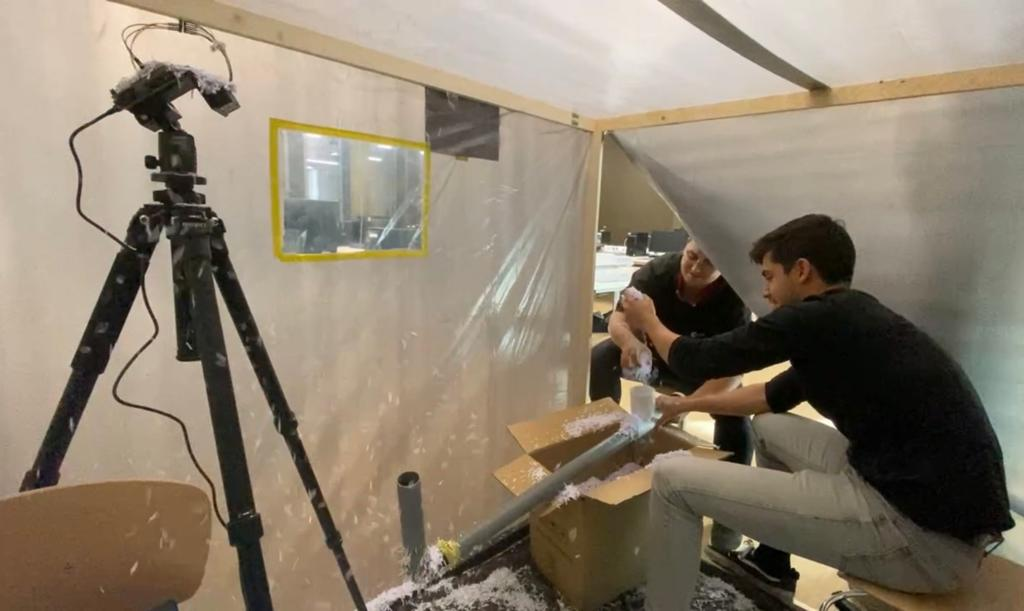
\includegraphics[width=0.75\textwidth]{Images/LiDAR/ErrorMesSetup.jpeg}
    \caption{Mise en place du test de perturbation}
    \label{fig:ErrorMesSetup}
\end{figure}

\subsubsection{Résultats du test}

\begin{figure}[H]
    \centering
    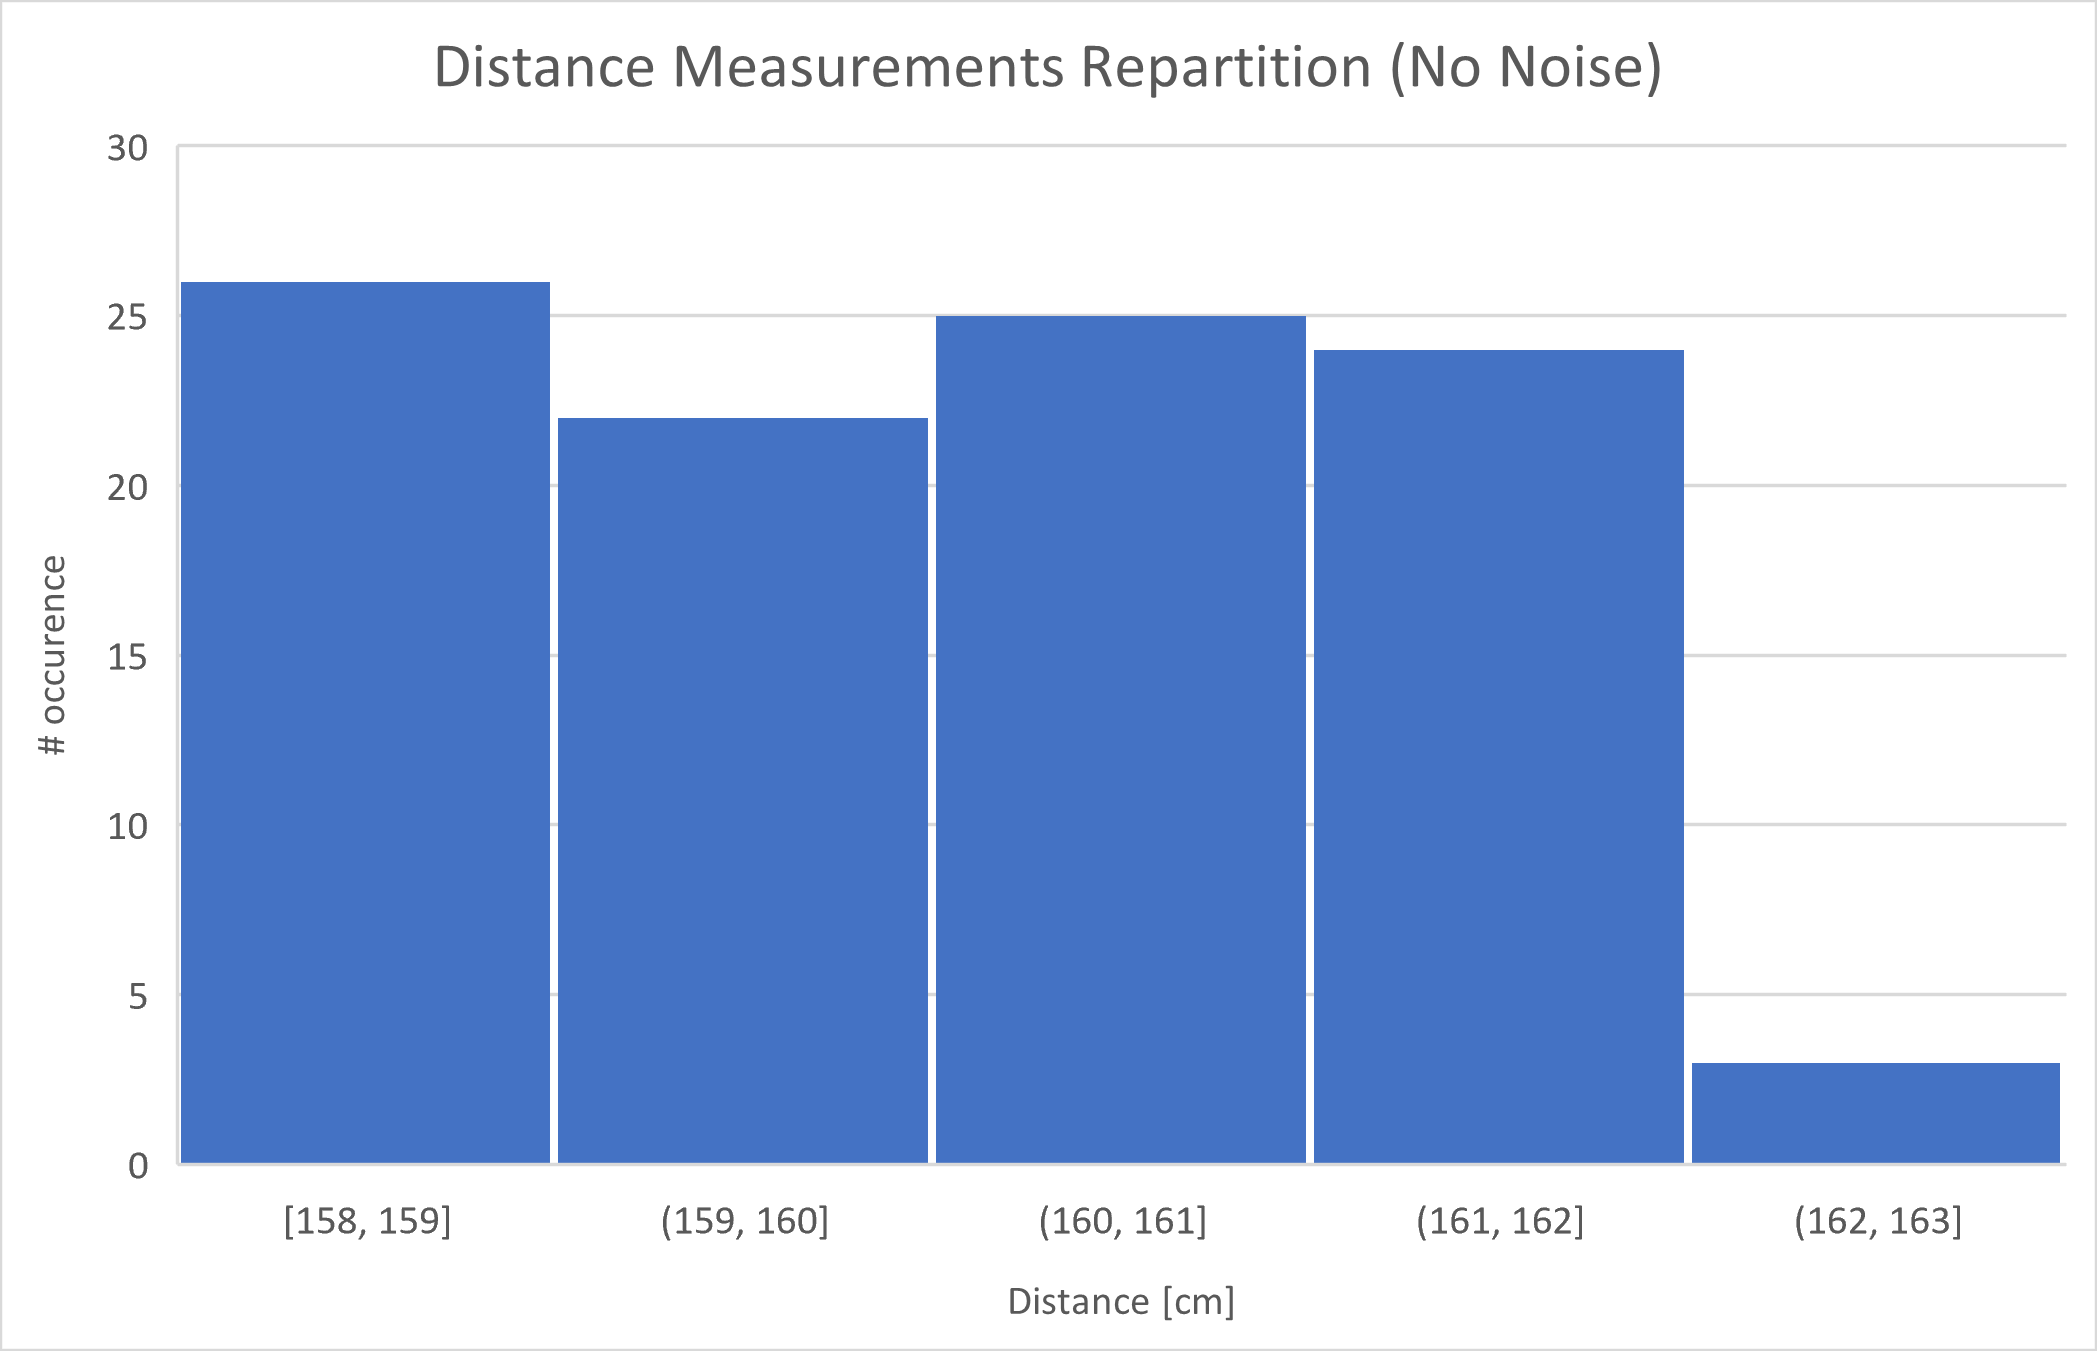
\includegraphics[width=0.8\textwidth]{Images/LiDAR/LiDAR_ErrorMes_NoNoise.png}
    \caption{Histogramme de la mesure de référence}
    \label{fig:ErrorMesRefDist}
\end{figure}

\begin{figure}[H]
    \centering
    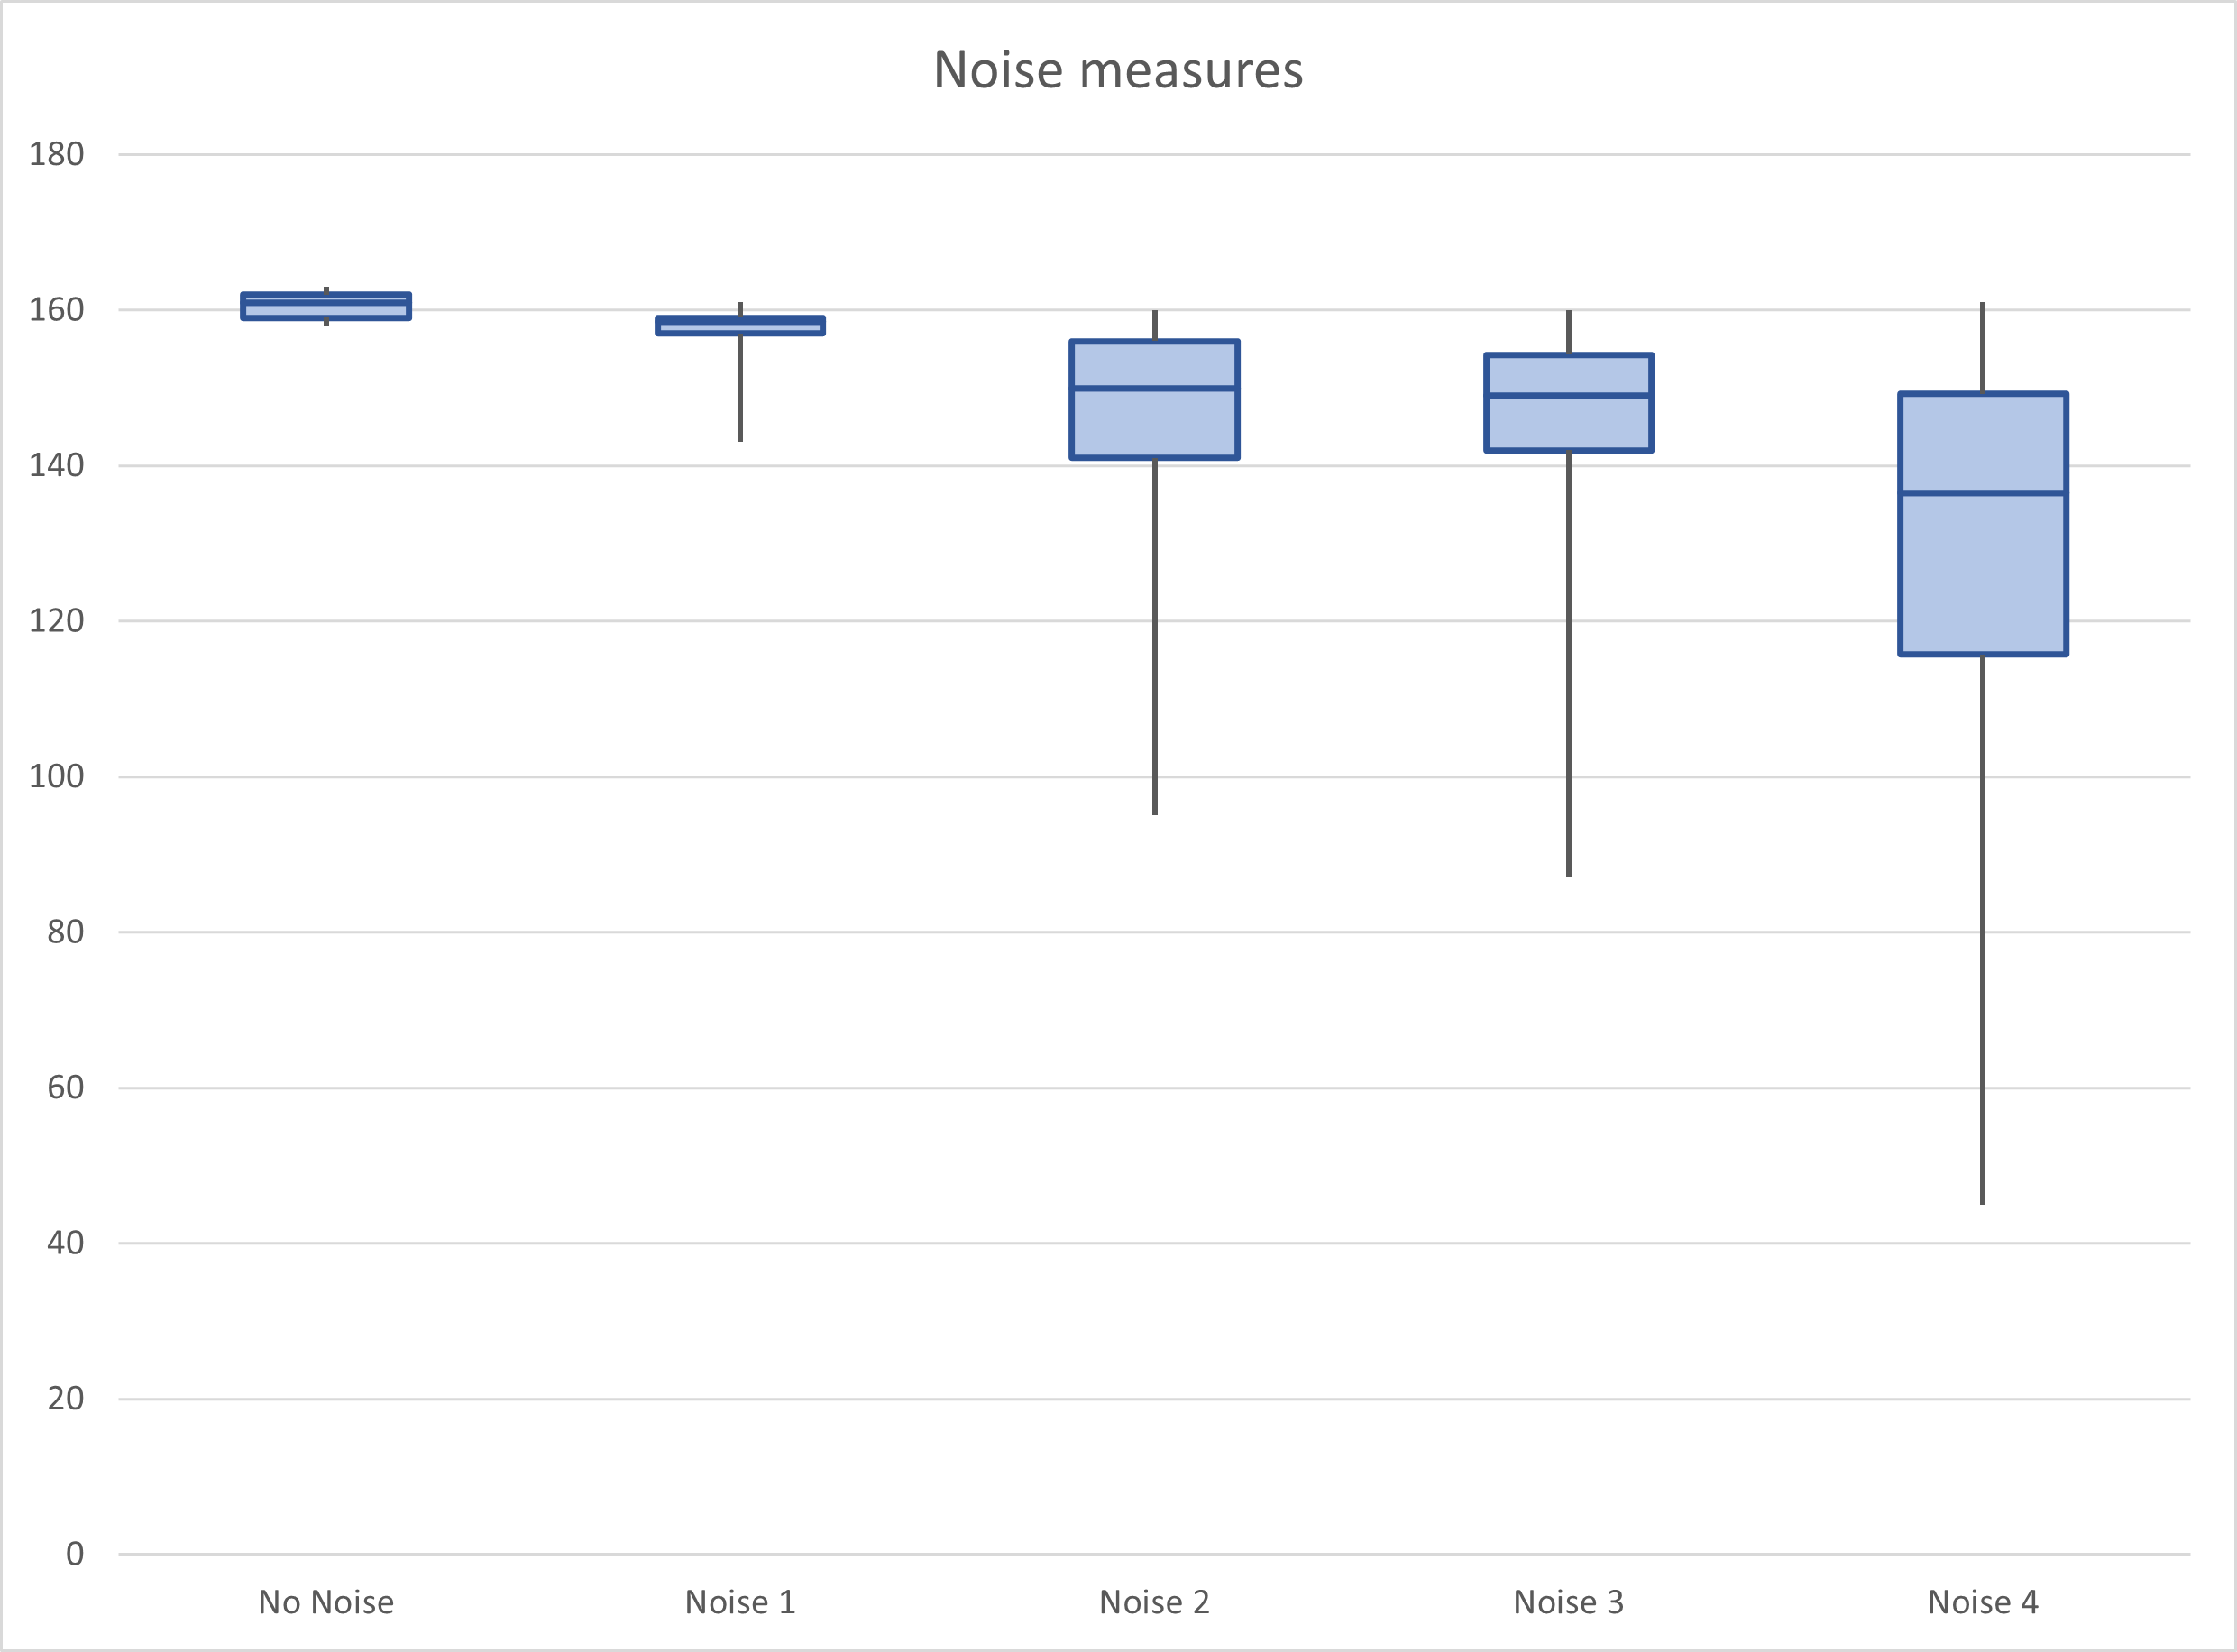
\includegraphics[width=0.8\textwidth]{Images/LiDAR/LiDAR_ErrorMes_Moustache.png}
    \caption{Comparaison des 5 mesures effectuées}
    \label{fig:ErrorMesMoustache}
\end{figure}

Les 5 mesures ont été regroupées en un seul graphe de type "Boîte à moustaches" afin de pouvoir
comparer avec plus d'aisance les mesures entre-elles. De gauche à droite, on retrouve une augmentation
graduelle du bruit généré par les opérateurs.

\begin{table}[H]
    \centering
    \begin{tabular}{|c|c|c|c|c|c|}
        \hline
        & No Noise & Noise 1 & Noise 2 & Noise 3 & Noise 4 \\
        \hline\hline
        Mean & 160.52 & 157.77 & 145.44 & 145.06 & 127.78 \\
        \hline
        Median & 161 & 158.8 & 150 & 149 & 136.5 \\
        \hline
        Max & 163 & 161 & 160 & 160 & 161 \\
        \hline
        
    \end{tabular}
    \caption{Différentes méthodes de calcul de distance (en cm)}
    \label{table:ComputingMethods}
\end{table}

Afin d'avoir la méthode la plus représentative possible de la distance au sol, trois solutions 
ont été envisagées. À partir de la série de mesures, nous avons calculé la moyenne, la médiane
ainsi que le maximum afin de déterminer laquelle de ces valeurs représente le plus la réalité.\\
//ANNEXE A : HISTOGRAMME DE CHACUNE DES MESURES

\subsubsection{Conclusion préliminaire} 

Premièrement, la figure \ref{fig:ErrorMesRefDist} montre l'histogramme des 100 mesures de référence au sol.
Elles s'avèrent plutôt rassurantes car on remarque que la répétabilité des mesures est respectée, avec
une précision typique de \textpm 2cm. La plupart des mesures sont réparties uniformément autour de 160cm.\par
On distingue ensuite sur la figure \ref{fig:ErrorMesMoustache} que le bruit de mesure a bel et bien augmenté
au fil des séries, représenté par la longueur des barres d'erreur. Comme l'indique le principe des boîtes
à moustache, le trait central du rectangle représente la médiane des valeurs, alors que les deux autres
sont le premier et troisième quartiles. Ainsi, les valeurs médianes des séries s'éloignent de plus en 
plus de la distance au sol (de référence).\par
Le but final de la figure \ref{fig:ErrorMesMoustache} est d'aider à déterminer quelle est la méthode
de mesure la plus efficace pour calculer des distances dans un environnement perturbé. On remarque
ainsi d'ores et déjà que la médiane n'est pas un outil fiable, puisque sa valeur d'éloigne de plus en
plus de la référence au fil des séries. Cependant, on voit facilement que les valeurs maximales de chaque
boîte s'approche très fortement de la distance de référence.\\
La table \ref{table:ComputingMethods} nous aide à y voir plus clair en ce qui concerne l'efficacité de ces
trois méthodes. Pour rappel, selon la mesure de référence, la distance au sol à mesurer est de 160cm.

\begin{description}
    \item[Moyenne] \hfill \\ 
    La moyenne représente la meilleure méthode dans le cas d'une mesure sans aucune 
    perturbation. Cependant, on voit que cette méthode devient très imprécise lorsque du bruit
    apparaît devant le capteur.
    \item[Médiane] \hfill \\ 
    Malgré le fait que la médiane soit généralement plus proche de la réalité par rapport 
    à la moyenne, elle est encore beaucoup trop éloignée de la vraie distance au sol. L'erreur est à 
    nouveau de plus en plus grande dès que les perturbations augmentent. 
    \item[Maximum] \hfill \\ 
    La méthode du maximum semble donner une valeur très proche de la vraie distance,
    et ce peu importe le niveau de perturbation devant le capteur. Il suffit en effet qu'une valeur
    de la série soit la mesure du sol pour que cette méthode fonctionne. Nous comptons donc sur le fait 
    que, statistiquement, on finisse toujours par faire au moins une mesure de la distance au sol dans 
    la série.
\end{description}

Il semblerait que pour le moment, la méthode du maximum obtienne les résultats les plus prometteurs.
Cependant, nous garderons ces 3 méthodes pour les tests suivants afin de confirmer ou non l'efficacité
des techniques de calcul.

\subsection{Stabilité en température des mesures}

Le capteur, intégré dans un boîtier étanche, sera soumis à des températures qui varient constamment,
de -20°C lors d'une nuit glaciale jusqu'à 30 voire 40°C à l'intérieur du boîtier, en plein soleil.
Il est important de savoir comment les mesures prises par le LiDAR vont être influencées par cette 
variation.\\
À titre d'exemple, imaginons que le système prenne une mesure de distance de référence afin d'être
prêt à mesurer des hauteurs de neige. Le soleil vient de se coucher, mais une température de 15°C
reigne encore dans le boîtier. Plus tard dans la nuit, alors qu'il fait -5°C, il commence à neiger.
Le système de détection se met en marche et commence à mesurer des offsets. Ces derniers seront
peut-être faussés par une différence de 20°C entre la mesure de référence et la mesure actuelle !

\subsubsection{Méthode}

Le LiDAR et la plaque de développement sont fixés sur un trépied et sont placés dans une chambre
climatique (de la marque \emph{Vötsch}, modèle 4010) afin de faire varier la température ambiante.
Comme décrit dans le paragraphe ci-dessus, le système sera soumis à des températures entre -20°C et
40°C. C'est pour cela que le capteur sera soumis à cette même plage de températures, par pas de 5°C.\\
La distance entre le capteur et la paroi opposée de la chambre climatique est de 47cm. Les mesures 
sont récupérées via le port COM qui lie la carte à l'ordinateur. La figure \ref{fig:TempError} montre 
la mise en place du test, avec le capteur à l'intérieur de la chambre.

\begin{figure}[H]
    \centering
    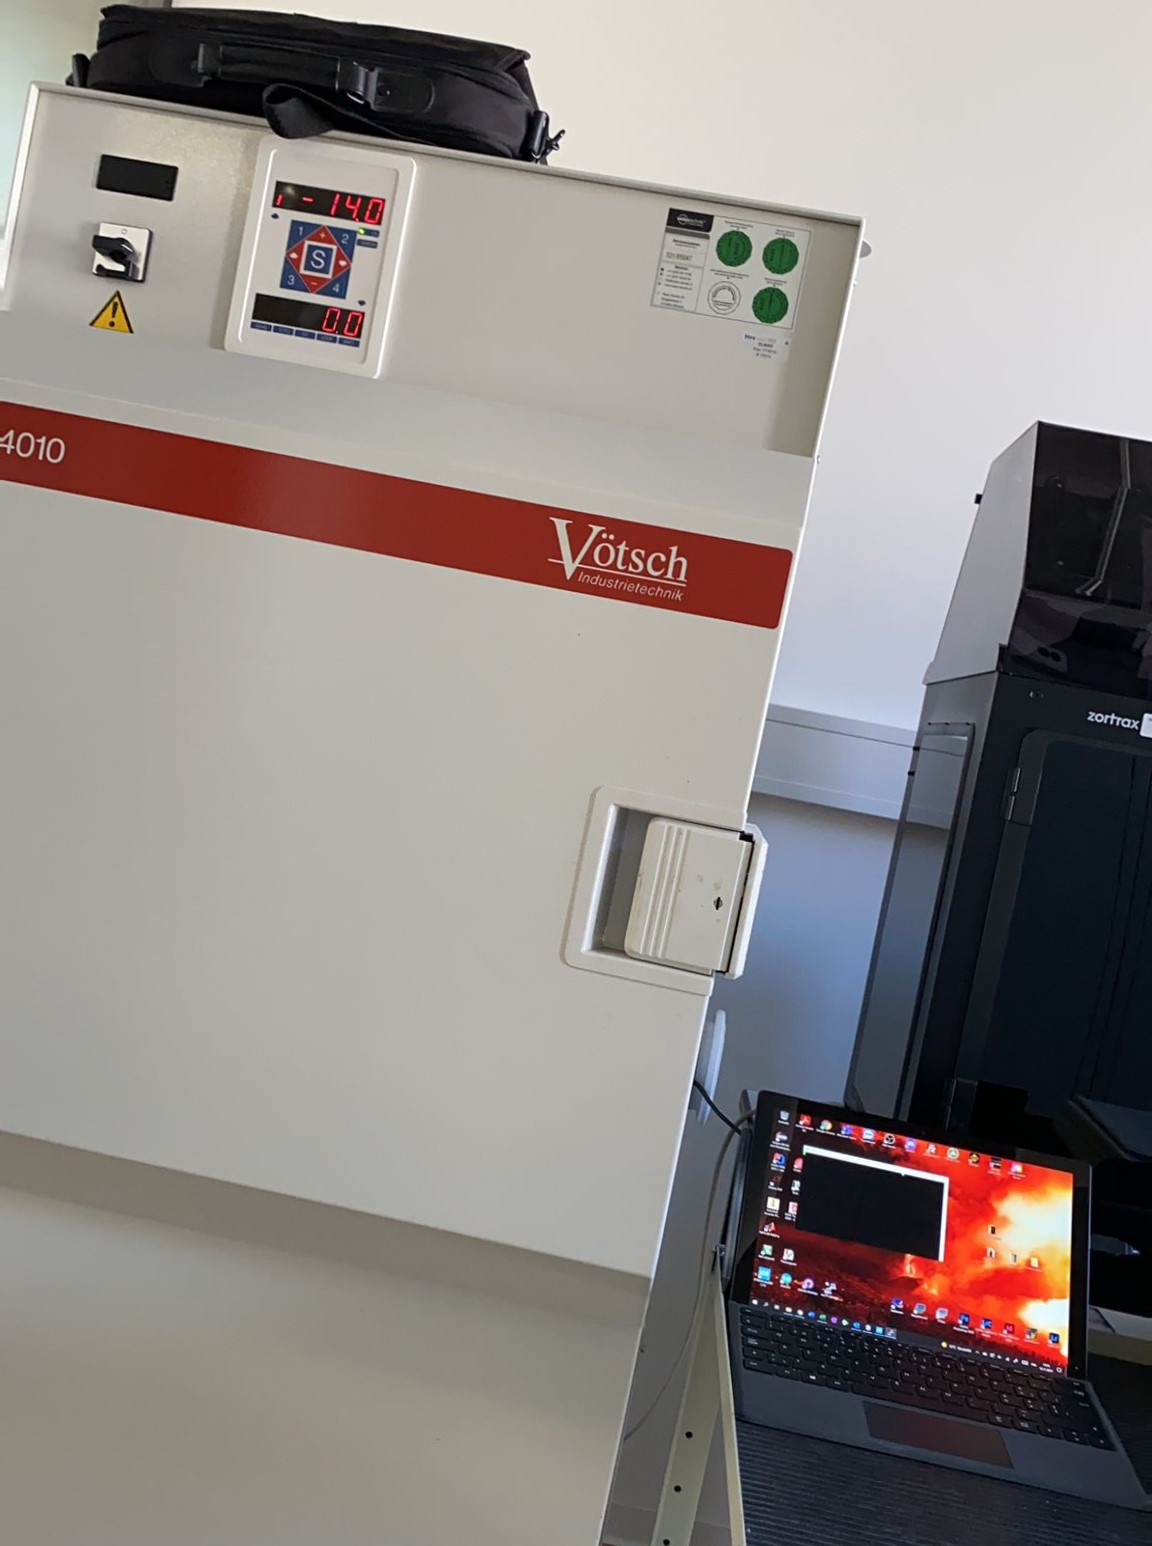
\includegraphics[width=0.5\textwidth]{Images/LiDAR/TempMes.jpeg}
    \caption{Mise en place du test en température}
    \label{fig:TempError}
\end{figure}

\subsubsection{Résultats du test}

\begin{figure}[H]
    \centering
    \includegraphics[width=0.8\textwidth]{Images/LiDAR/LiDAR_TempStabilityGraph.png}
    \caption{Graphe de stabilité en température du LiDAR}
    \label{fig:TempErrorGraph}
\end{figure}

Le test a été réalisé à partir d'une température de -15°C et non pas de -20°C. En effet, la chambre
climatique utilisée n'était pas en mesure d'atteindre cette consigne dans un temps raisonnable.\\
Les trois méthodes décrites dans le test précédent ont été reprises afin de mieux comprendre la
répartition des valeurs mesurées.

\subsubsection{Conclusion préliminaire} 

Il semblerait que le capteur soit relativement peu influencé par la variation de température. En
effet, en plus de sa résolution fixe de 1cm, nous avons une erreur typique de \textpm 2cm autour
de la valeur réelle.\\
Cependant, on constate tout de même que la moyenne et la médiane sont plus influencées que la méthode
du maximum. On peut ainsi conclure que le capteur est plutôt stable en température, surtout si on
utilise le maximum comme méthode de mesure.\par 
On peut considérer finalement que le capteur est fiable pour une mesure de référence et de hauteur
de neige prises à des températures différentes, comme cette différence est noyée dans sa précision
typique.

\subsection{Mesure de hauteur en laboratoire}

Maintenant que nous avons caractérisé ce capteur pour plusieurs situations, nous pouvons procéder aux
véritables mesures d'épaisseur en laboratoire. En effet, il faut à présent vérifier si la méthode de
calcul de la section \ref{sec:MethodeDeMesure} est réalisable en condition de laboratoire dans un premier
temps.

\subsubsection{Méthode}

Pour effectuer ce test, le capteur est placé dans le banc de test à une hauteur $h$ de 133cm au-dessus
du sol. L'angle $\alpha$ du LiDAR a été fixé à 60°, alors que l'angle $\beta$ est de 0°. Ces informations 
ont été fournies au programme de test afin de calculer des bons offsets. La figure \ref{fig:OffsetMes_Labo}
montre la préparation au test.\\
Le but est de mesurer tout d'abord une distance de référence au sol, sans aucun obstacle ni bruit de
mesure. Ensuite, une fois la plaque placée, on effectue quatre mesures différentes, la première sans
bruit puis avec un bruit graduel généré par les opérateurs.\\
L'obstacle utilisé est une plaque en mousse blanche de protection, d'une épaisseur de 6.6cm.

\begin{figure}[H]
    \centering
    \includegraphics[width=0.5\textwidth]{Images/LiDAR/OffsetMes_InLab.jpeg}
    \caption{Mise en place du test de mesure d'épaisseur}
    \label{fig:OffsetMes_Labo}
\end{figure}

\subsubsection{Résultats du test}

\begin{figure}[H]
    \centering
    \includegraphics[width=0.8\textwidth]{Images/LiDAR/LiDAR_OffsetMes_Moustache.png}
    \caption{Boîte à moustache des mesures d'épaisseur}
    \label{fig:OffsetMes_Moustache}
\end{figure}

Il est important de noter que pour la série de mesure \emph{Noise 3}, la valeur maximale n'atteint
pas celle des autres séries. Cela est dû majoritairement au fait qu'une couche de 2cm de confettis
se sont accumulés sur la plaque au fil des mesures.

\begin{figure}[H]
    \centering
    \includegraphics[width=0.8\textwidth]{Images/LiDAR/LiDAR_OffsetMes_PerMethods.png}
    \caption{Résultat des calculs d'offset par méthode}
    \label{fig:OffsetMes_PerMethod}
\end{figure}

\subsubsection{Conclusion préliminaire} 

Le graphe \ref{fig:OffsetMes_Moustache} montre la répartition des mesures effectuées sous la forme d'une
boîte à moustache. Cela permet de représenter facilement la répartition des mesures autour de la médiane.\\
On remarque sur les séries \emph{Noise 1} à \emph{Noise 3} que du bruit a bien été généré par les
opérateurs, ce qui n'est pas le cas pour les deux premières séquences de mesure. Hormis cela, le graphe
est très similaire aux tests dans un environnement perturbé, à la section \ref{fig:MesNoise}. On retrouve
en effet une médiane qui s'éloigne de plus en plus de la vraie distance, alors que le maximum s'approche
le plus de la réalité.\par
On voit sur la figure \ref{fig:OffsetMes_PerMethod} l'épaisseur calculée à l'aide de la méthode de la section
\ref{sec:MethodeDeMesure} pour les 3 solutions proposées, à savoir la moyenne, la médiane et le maximum. Ce
calcul d'offset a été réalisé pour les quatre séries de mesures à disposition, avec un bruit graduel. On 
peut ici conclure que la méthode du maximum est la plus proche de la réalité. Pour cette raison, elle sera
utilisée pour les tests sur le terrain.

\subsection{Mesure de hauteur en situation réelle}

Après avoir prouvé le fonctionnement du capteur en laboratoire, il est essentiel de le tester en conditions
réelles, sous la neige. Pour ce faire, des tests ont été réalisés la nuit du 3 au 4 décembre 2021 à Ayent.
Un boitier temporaire a été confectionné afin de protéger le LiDAR et la carte de développement des 
précipitations.

\subsubsection{Méthode}

Le boitier a été installé sur un trépied à 140cm au-dessus du sol, sous un couvert, à l'abri de la majorité
des flocons. Le LiDAR pointe vers le sol avec un angle de 45° par rapport à la verticale, donnant une
distance de 197cm entre le capteur et la route. Les données récoltées sont enregistrées via un câble 
USB sur un ordinateur.\\
Le but est de mesurer des épaisseurs de neige en partant de 0cm (la route a été nettoyée au préalable)
afin de mettre à l'épreuve l'efficacité du capteur et de nos méthodes de mesure. Chaque mesure d'épaisseur 
est réalisée chaque 30 secondes, et ce pendant plus d'une heure. En parallèle, une double-mètre est posé 
dans la neige afin de relever périodiquement la hauteur de neige présente sur la route. Une mesure
qualitative du débit de neige est aussi effectuée. La figure \ref{fig:RealTest_Setup} montre la mise en
place du test. Le double-mètre et l'ordinateur ne sont pas visibles ici.

\begin{figure}[H]
    \centering
    \includegraphics[width=0.75\textwidth]{Images/LiDAR/ReadTests_Setup.jpeg}
    \caption{Mise en place du test en condition réelle}
    \label{fig:RealTest_Setup}
\end{figure}

\subsubsection{Résultats du test}

\begin{table}[H]
    \centering
    \begin{tabular}{|c|c|c|c|c|}
        \hline
        Mesure n° & Hauteur réelle [cm] & Hauteur mesurée [cm] & Type de précipitation & Heure \\
        \hline\hline
        1 & 0 & 0 & Petits flocons & 04h28 \\
        \hline
        2 & 0.5 & 0.71 & Petits flocons & 04h39 \\
        \hline
        3 & 0.8 & 1.41 & Quelques gros flocons & 04h48 \\
        \hline
        4 & 1.5 & 1.41 & Quelques gros flocons & 05h00 \\
        \hline
        5 & 2 & 2.12 & Quelques gros flocons & 05h08 \\
        \hline
        6 & 2.5 & 2.12 & Quelques gros flocons & 05h14 \\
        \hline
        7 & 2.8 & 2.86 & Quelques gros flocons & 05h21 \\
        \hline
        8 & 3 & 2.86 & Quelques gros flocons & 05h32 \\
        \hline
        
    \end{tabular}
    \caption{Mesures relevée lors du test}
    \label{table:SnowingState}
\end{table}

\begin{figure}[H]
    \centering
    \includegraphics[width=0.75\textwidth]{Images/LiDAR/ReadTests_Results.png}
    \caption{Résultat des mesures effectuées}
    \label{fig:RealTest_Results}
\end{figure}

La température lors des mesures oscillait entre -2°C et 0°C, sans aucun vent.\par 
Afin de réaliser la courbe \emph{Mesure réelle} de la figure \ref{fig:RealTest_Results}, une interpolation
linéaire a été utilisée entre les différents points de mesure.

\subsubsection{Conclusion préliminaire} 

Après avoir passé plusieurs heures dans un froid glacial à mettre à l'épreuve notre projet, nous avons 
enfin pu obtenir des résultats.\\
Le tableau \ref{table:SnowingState} montre les différentes heures de mesures, mettant notamment en évidence
l'erreur entre la valeur réelle et mesurée. Malgré une légère oscillation lors d'un changement proche
de valeur (figure \ref{fig:RealTest_Results}), on peut conclure que le LiDAR arrive bel et bien à mesurer 
une hauteur de neige, et ce depuis le sol.\par 
On constate par la même occasion que le pas de mesure du capteur dépend effectivement de son angle par 
rapport à la verticale.

\chapter{Mécanique}

\section{Implémentation}
Pour tester les algorithmes de mesure avec des vidéos sur le terrain,
Dr. Mudry Pierre-André et M. Matter Fabien nous on aimablement laissé accès à
la caméra de notre projet parent \emph{VibroSnow\cite{VibroSnow}} et nous
les remercions énormément.

\subsection{Récupération des vidéos}
La caméra de \emph{VibroSnow} détecte le passage d'objet (voitures, chute de neige,...) et
enregistre une vidéo qui est ensuite transmise à un serveur \emph{Windows}.
Bien que l'accès aux vidéos nous a été donné, nous ne pouvons pas aller chercher les vidéos
directement sur le serveur \emph{Windows} car il est utilisé pour d'autres projets auxquels nous
n'avons pas accès.\\
Il a donc fallu créer un script \emph{Powershell}, transferant chaque jour les vidéos
cumulées sur le serveur \emph{Windows} vers un serveur auquel nous avons accès.
Un \emph{Raspberry Pi} a été mis en place comme serveur pour récuperer les vidéos.

\subsection{Mesure du débit de chute de neige}
La méthode utilisée pour détecter les chutes de neige se décompose ainsi :
\begin{description}
    \item[Soustraction de deux images] \hfill \\
    pour isoler les éléments qui ont bougé entre les deux images
    \item[Seuillage des niveaux de blancs sur l'image] \hfill \\
    pour accentuer les chutes de neige
    \item[Calcul du ratio de pixels blancs] \hfill \\
    pour avoir un nombre correspondant au débit de chute de neige    
\end{description}

\begin{figure}[H]
    \begin{subfigure}{.45\textwidth}
        \includegraphics[width=\linewidth]{Images/computer_vision/snowfall/original.png}
        \caption{Image originale}
        \label{fig:Snowfall_original}
    \end{subfigure}
    \hfill
    \begin{subfigure}{.45\textwidth}
        \includegraphics[width=\linewidth]{Images/computer_vision/snowfall/noise.png}
        \caption{Image avec neige isolée}
        \label{fig:Snowfall_noise}
    \end{subfigure}
    \hfill
    \centering
    \begin{subfigure}{.45\textwidth}
        \includegraphics[width=\linewidth]{Images/computer_vision/snowfall/snowfall.png}
        \caption{Image seuillée avec calcul du ratio de pixels blancs (9.05\% ici)}
        \label{fig:Snowfall_thres}
    \end{subfigure}
    \caption{Étapes de la mesure de débit de chute de neige}
    \label{fig:Snowfall_algorithm}
\end{figure}
\newpage

\subsection{Détection de route enneigée}
Deux méthodes ont été testées pour détecter si la route est enneigée ou non.\\
La première réalise un simple seuillage des niveaux de blancs, et un calcul
du ratio des pixels blancs sur l'image. On récupère plusieurs images et on
calcul la moyenne du ratio de blanc sur toute les images.
Cette moyenne est ensuite comparée à une moyenne similaire réalisée sur une
vidéo de la route déneigée, en vérifiant qu'on se trouve au même moment de
la journée (jour/nuit, matin/après-midi).\\
La deuxième est identique, à l'exception d'une suppression du bruit réalisée
avant le seuillage. Cette suppresion du bruit reprends la méthode d'isolation
de neige utilisée pour mesurer le débit de chute de neige et soustrait cette image
de bruit à l'image originale. Cette méthode demande un peu plus de calculs mais peut
potentiellement générer un résultat plus fiable.

\begin{figure}[H]
    \begin{subfigure}{.45\textwidth}
        \includegraphics[width=\linewidth]{Images/computer_vision/snowOnRoad/ref_original.png}
        \caption{Image de référence originale}
        \label{fig:SnowOnRoad_ref_original}
    \end{subfigure}
    \hfill
    \begin{subfigure}{.45\textwidth}
        \includegraphics[width=\linewidth]{Images/computer_vision/snowOnRoad/ref_thres.png}
        \caption{Image de référence seuillée}
        \label{fig:SnowOnRoad_ref_thres}
    \end{subfigure}
    \caption{Image de référence}
    \label{fig:SnowOnRoad_ref}
\end{figure}

\begin{figure}[H]
    \begin{subfigure}{.45\textwidth}
        \includegraphics[width=\linewidth]{Images/computer_vision/snowOnRoad/test_original.png}
        \caption{Image de test originale}
        \label{fig:SnowOnRoad_test_original}
    \end{subfigure}
    \hfill
    \begin{subfigure}{.45\textwidth}
        \includegraphics[width=\linewidth]{Images/computer_vision/snowOnRoad/test_thres.png}
        \caption{Image de test seuillée}
        \label{fig:SnowOnRoad_test_thres}
    \end{subfigure}
    \hfill
    \begin{subfigure}{.45\textwidth}
        \includegraphics[width=\linewidth]{Images/computer_vision/snowOnRoad/test_denoised.png}
        \caption{Image de test avec suppression de bruit}
        \label{fig:SnowOnRoad_test_denoised}
    \end{subfigure}
    \hfill
    \begin{subfigure}{.45\textwidth}
        \includegraphics[width=\linewidth]{Images/computer_vision/snowOnRoad/test_denoisedThres.png}
        \caption{Image de test avec suppression de bruit et seuillée}
        \label{fig:SnowOnRoad_test_denoisedThres}
    \end{subfigure}
    \caption{Image de test}
    \label{fig:SnowOnRoad_test}
\end{figure}
\newpage

\chapter{Synthèse des résultats}
\section{LiDAR}
Une batterie de tests a été effectuée afin d'attester du bon fonctionnement du LiDAR dans les conditions
attendues.\par
En effet, on remarque que le capteur est capable de fonctionner dans la plage utile de 2 à 
4 mètres. Il serait cependant préférable d'éviter d'avoir une distance trop grande entre ce dernier et 
la route, comme sa mesure diverge très vite de la réalité. \\
De la même manière, le LiDAR a été mis à l'épreuve dans le banc de test en laboratoire. Sur une série 
d'une centaine de mesures, il était parfaitement capable de mesurer une distance au sol, et ce peu importe 
le débit de fausse neige devant le capteur. Cette information est essentielle pour un fonctionnement en
condition réelle. De cette manière, nous savons que la neige ou le brouillard ne poseront pas de problèmes 
pour effectuer les mesures. La méthode de mesure du maximum a par ailleurs été retenue.\\
Comme ce projet est à même de devoir résister à de grandes variations de température entre le jour et
la nuit. Cependant, cette différence ne doit en aucun cas avoir des répectutions sur les mesures effectuées.
Heureusement, il semble que le capteur soit stable en température, restant majoritairement dans son 
erreur typique.\\
Après que les tests ci-dessus soient validés, nous avons pu nous concentrer sur une méthode de mesure de 
hauteur en laboratoire. Nous avons ainsi constaté que le capteur arrive à calculer la hauteur d'un élément,
même avec du bruit généré devant lui. Il faut cependant faire attention à la porosité du matériau mesuré. En
effet, certaines épaisseurs ont été fortement faussées. Cette étape a aussi permis de définitivement valider
la méthode du maximum pour le test suivant.\\
Finalement, le 4 décembre 2021, nous avons pu faire une nuit de mesure sur le terrain. Le LiDAR a été en
mesure de calculer la hauteur de neige présente sur la route, et ce avec une
précision de 7 milimètres! Ce test final a permis de valider le \emph{proof of concept} de cette méthode. De plus amples
recherches et essais doivent être effectués afin de totalement valider ou abandonner ce capteur, mais les
résultats actuels sont prometteurs.\par 
Il est important de noter que, comme prévu, le LiDAR ne fonctionne pas de jour, même lorsque le ciel
est complètement couvert. Cela ne pose en aucun cas un problème. En effet, ce projet est fait pour 
majoritairement fonctionner la nuit.

\subsection{Problèmes rencontrés}
Nous savons que le LiDAR a des difficultés à mesurer des distances sur des matériaux poreux. Cependant,
les essais sur le terrain avec de la véritable neige n'ont monté aucune erreur. Il serait nécessaire
d'approfondir les recherches afin de déterminer si certaines neiges peuvent provoquer ce problème.

\section{Computer Vision}
La \emph{Computer Vision} qui devait initialement servir plutôt de redondance au \emph{LiDAR} fournit
finalement des résultats très suprenant avec des algorithmes très simples.\\
La mesure du débit de chute de neige est fonctionnelle, bien que perfectible avec des données météos précises.\\
La détection de route enneigée est une réussite, l'algorithme est très simple et peut tourner sur un
processeur rudimentaire. Elle fournit une mesure très importante et le fait à la perfection.\\
La vision par ordinateur permet donc de palier parfaitement aux problèmes du \emph{LiDAR},
c'est à dire : les mesures durant la journée, et les erreurs liées à la mesure sur un point (p. ex: caillou sur le point de mesure).\\
Si on imaginait un système encore plus simpliste, la \emph{Computer Vision} pourrait être le seul outil de mesure.

\subsection{Problèmes rencontrés}
\subsubsection{Caméra}
Au départ, pour tester rapidement l'idée de la mesure de débit, nous avions imaginés filmer notre session
de mesure avec un ordinateur, puis comparer les données de bruit du LiDAR avec le débit estimé par
la caméra. Hors les webcams utilisées n'avaient pas de possibilités de désactivation de l'autofocus,
du réglage automatique du diaphragme et rendaient les vidéos capturées inutilisables.\\
Il a donc été primordiale de récupérer des données d'une caméra bien plus fiable, et sur le terrain.
Nous remercions encore une fois Dr. Mudry Pierre-André et M. Matter Fabien de nous avoir donné
l'accès aux vidéos de la caméra du projet parent \emph{VibroSnow\cite{VibroSnow}}.
\subsubsection{Données météos}
Une demande d'accès aux données de \emph{MeteoSwiss} a été visée et signée par M. Cyrille Bezençon et transmise
par la poste vers \emph{MeteoSwiss}. Cependant l'autorisation a tardé à arriver et les données météos
n'ont pas pu être utilisées pour améliorer la reconnaissance du débit de chute de neige.

\section{Mécanique}
Grace à un banc de test comprenant une cage d’essai et un canon à confettis. Plusieurs séries de mesures 
concluantes ont pu être réalisées. Le débit de neige produit par le canon étant réglable, il augmente les 
possibilités de mesures. La cage permet de contenir les nuages de confettis sans dégrader les conditions 
de travails des autres usagers de la salle.\\
Différents designs de boitier ont été imaginés avant d’arriver à la solution finale. L’étanchéité fut la 
partie plus problématique lors de la conception. L’utilisation de joint torique pincé permit de résoudre 
ces problèmes. L’ABS étant une matière très simple à injecter, la fabrication des pièces du boitier serait 
corolaire. Le support du boitier permet de régler à la fois l’élévation et l’azimut du boitier. La partie 
amovible supérieure permet un très bon accès à la partie du module électronique. Elle se verrouille facilement 
grâce à une fermeture par grenouillère. L’ouverture est verrouillée grâce à la serrure incrustée dans la 
fixation.\\
Le module électronique se fixe simplement dans le boitier à l’aide de 4 vis. Une pièce mécanique permet 
de loger les batteries. Au-dessus des batteries, une plaque permet la fixation du capteur Lidar 
et des PCB. Suffisamment d’espace est prévu autour du module afin de pouvoir disposer aisément le câblage. 
La simplicité du module permet une manipulation rapide et simple des différents éléments.

\part{Gestion}

\chapter{Résumé}
\section{Idée commerciale}
LoRaSnow est une solution autonome de détection de hauteur de neige. 
Il arrive parfois que les routes mettent du temps à être déneigées, ou que le salage soit trop
faible, conduisant à une chaussée glissante et dangereuse. De plus, une répartition inhomogène du manteau neigeux sur une
région peut rendre la tâche compliquée, surtout en montagne. LoRaSnow apporte un monitoring constant
des niveaux de neige sur la route et du débit de neige à des points clés ainsi que les possibilités de verglas.\\[0.2cm]
Grâce à un réseau de capteurs sur une région, il devient possible d’optimiser la courses des chasses-neige
et de cibler les axes en plus grandes difficultés, de même que d’offrir l’opportunité d’effectuer des sa-
lages préventifs, avant que du verglas ne se forme.\\[0.2cm]
Se présentant sous forme d'abonnement annuel, il suffit au client de souscrire et de bénéficier
d'un service de surveillance des routes. Le client n'aura pas à se soucier d'éventuelles pannes, installations
et infrastructures, tout est compris dans l'abonnement.

\section{Domaine d'activité}
Le domaine d'activité principal est la détection de hauteur de neige sur route de montagne.

\section{Marché}
Des communes, comme Ayent, ont manifesté leur intérêt pour une solution
de détection du niveau de neige sur route.
Des entreprises privées de déneigement bénéficieraient de LoRaSnow pour
optimiser leur service de déneigement et améliorer la qualité du service
fourni.\\
Pour lancer le produit, il faudra d'abord cibler les communes avec stations de ski,
qui ont plus de moyens et de raisons de se tourner vers l'innovation.\newpage

\section{Analyse des risques}
\begin{figure}[H]
    \centering
    \includegraphics[width=\linewidth]{Images/business/risiko.PNG}
    \caption[]{Analyse des risques}
    \label{fig:risiko}
\end{figure}

Il est possible qu'une installation soit endommagée ou détruite par la faune, l'environnement
ou par un simple vandale. Les causes naturelles sont trop improbables pour être considérées.
Le vandalisme sera paré par des installations très discrètes: afin d'éviter que les automobilistes
ne s'arrêtent, pensant qu'il s'agit d'un nouveau radar de la police et le vandalisant en conscéquence.
Une assurance est également à prévoir si une installation discrète n'est pas possible.\\[0.2cm]
L'appareil étant prévu pour effectuer des mesures exposé aux précipitations, il va inévitablement se trouver couvert
d'une grande couche de neige. La casquette du boitier permet d'éviter l'enneigement de la vitre et
le montage du boitier est suffisamment solides pour supporter de fortes charges, rendant ce risque insignifiant.\\[0.2cm]
Il faut prévoir une redondance pour le réseau LoRaWAN. Une panne des passerelles n'est pas impossible, et si cela arrive,
tous les appareils dans la nature ne pourraient plus transmettre leurs données. Il faut donc toujours avoir
un minimum de 3 appareils qui couvrent une région afin d'éviter une perte de couverture.\\[0.2cm]
La pénurie de semi-conducteurs persiste et pourrait s'éterniser. Pour éviter de
ne pas pouvoir respecter les commandes des clients, il pourrait être préférable d'attendre quelques années avant
d'envisager l'industrialisation et commercialisation du projet.

\chapter{Produits et services}
\section{Description du produit}
LoRaSnow est un projet pilote de détection de hauteur de neige sur route, de débit
de chute de neige ainsi que des risques de verglas.
L'objectif est de fournir une solution de montioring de l'état d'un segment de route.
Implémenter un réseau de modules LoRaSnow permettrait donc de surveiller une région entière et d'offrir
une meilleure gestion des ressources lors de la période hivernale, tant bien pour une administration
publique que pour une entreprise privée.\\
LoRaSnow utilise le protocole LoRaWAN pour communiquer les données sur le cloud, permettant ainsi
d'être installé n'importe où sans nécessiter d'infrastructure (internet ou électricité) au préalable.\\
Lorsque la neige commence à tomber, ou qu'une couche importante de neige est présente
sur une route, une alerte est transmise au client, lui ofrrant la possibilité d'être informé de la situation
sans devoir être actif devant un terminal. Cela permettrait d'éliminer les besoins de personnel
de piquet durant la nuit.


\section{Détection de hauteur de neige}
En utilisant un mélange de solutions lasers et de vision par ordinateur,
LoRaSnow permet une détection innovante et efficace de la couche de neige
présente sur un segment de route.

\section{Mesure du débit de chute de neige}
Toujours en utilisant la vision par ordinateur, une indication correcte et fiable
du débit de chute de neige en temps réel donne des informations sur les chutes de neige
sur la région, minimisant les risques de surprises.

\section{Détection du givre}
En intégrant une mesure de l'humidité ainsi qu'une mesure de la température
du bitume, couplé aux prévisions météos, LoRaSnow offre une prévision
de verglas efficace.

\section{Pourquoi nous ?}
Nous apportons une solution simple et autonome à un problème complexe et inexploré,
problème sur lequel nos prédécesseurs n'ont pas trouvé de solution fonctionnelle.

\chapter{Marché et Contexte}
\section{Qui bénificie du déneigement des routes}
Pour comprendre qui compose notre clientèle, il est important de comprendre à qui
bénéficie le déneigement des routes.

\begin{figure}[H]
    \centering
    \includegraphics[width=0.25\linewidth]{Images/business/beneficiaires.png}
    \caption[]{Bénéficiaires du déneigement}
    \label{fig:beneficiaires}
\end{figure}

\begin{description}
    \item[Tourisme] \hfill \\
    Si vous êtes en vacances en station, ne pas pouvoir profiter d'une journée à ski car
    les routes ne sont pas déneigées serait le comble. C'est pourquoi tous les commerces
    et communes des régions touristiques ont besoin de route impeccables en tout temps.
    \item[Communes] \hfill \\
    Une route déneigée, c'est une route sur laquelle vous évitez des accidents dus à la neige.
    C'est une route qui ne sera pas bloquée car une voiture est à l'équerre et bloque le car postal.
    C'est la mission d'une commune d'entretenir ses routes pour assurer la sécurité de ses citoyens.
    \item[Entreprises] \hfill \\
    Un boulanger a besoin de sa livraison tôt le matin. S'il ne l'a pas reçue, il ne pourra
    pas faire son pain à temps pour ses clients du matin. Il est donc fondamental que la route
    permette au livreur d'arriver à temps.
    Un opticien, avec seulement 2 employés, peut se retrouver à ne pas pouvoir ouvrir à l'heure
    si tout le monde est coincé à cause de la neige.
    \item[Citoyens] \hfill \\    
    Personne n'a envie de passer 15 minutes à déneiger sa voiture, pour finalement trouver une
    route en piteux état.
\end{description}

\section{Analyse de la clientèle}
\subsection{Communes}
Les administrations publiques verront en ce projet la possibilité de superviser
un territoire parfois compliqué (par exemple, les fonds de vallée,
routes de montagnes, etc...) et d'efficacement déneiger ou saler
afin que la chaussée soit prête à accueillir des automobilistes dès que possible.
Par exemple, la commune d'Ayent, étant très vaste et possédant des zones
où l'accès est compliqué, fait face au problème de la répartition inhomogène
des chutes de neige. Durant la nuit, il est donc contraignant d'envoyer
quelqu'un contrôler chaque zone. Des allers-retours inutiles peuvent être
évités grâce à un réseau de capteurs.
De plus, malgré la mise en place de personnel de piquet, il est possible
d'être surpris par des chutes de neige non annoncées par la météo.

\subsection{Entreprise privée}
De nombreuses entreprises fournissent des services de déneigement pour particuliers.
Installer des capteurs chez les clients (par exemple devant un boulanger),
permettrait de mieux planifier le déneigement, et ainsi d'améliorer la qualité
du service offert aux particuliers.
Notre solution permet également de minimiser les temps de sortie des véhicules,
et ainsi réaliser des économies.
Intégrer à tous leurs clients, LoRaSnow donnera une vue d'ensemble de l'état
des routes de leurs clients, optimisant par la même occasion leur parcours.
\newpage

\section{Analyse du marché}
\subsection{Demande}
La demande pour une telle solution est déjà présente, notamment en Valais.
La commune d'Ayent a déjà fait savoir son intérêt pour ce type de détection.

\subsection{Offres présentes sur le marché}
Actuellement, aucune offre comparable directement avec la nôtre n'est disponible.

\section{Analyse des partenaires}
\subsection{Eurocircuit}
Eurocircuit, leader européen dans la production de circuits imprimés sur mesures,
partenaire de choix pour la réalisation de produits électronique.
À noter que ce partenaire propose aussi un service de montage électronique,
ce qui nous permet de faire sous-traiter cette partie compliquée pour
un coût plus faible qu'en Suisse.

\subsection{Pfefferlé Sion}
Pfefferlé serait notre fournisseur de visserie et autre quincailleries (p. ex: la grenouillère du boitier).
Leur proximité est un avantage pour réduire les coûts et alimenter l'économie locale.

\subsection{Protolabs}
Protolabs est un fabricant de moule à injection plastique. Il offre la possibilité de fabriquer des
moules pour des petites productions (env. 1000 unités).
C'est un partenaire très important pour assurer une production de boitier bon marché et fiable.

\subsection{Boschung}
Boschung est une entreprise spécialisée dans les solutions de surveillance des routes et
notamment du déneigement. Ils proposent déjà un système de détection de verglas
sur les routes, mais sont relativement chers. Nous pourrions collaborer
afin de proposer nos solutions pour améliorer leurs gammes de produits.

\section{Analyse de la concurrence}
\subsection{Boschung}
Boschung, bien qu'un potentiel allié stratégique, pourrait devenir notre concurrent
principal. La détection de neige sur route est un domaine dans lequel ils cherchent à
s'implenter. De plus, ils possèdent un carnet de clients bien fourni et un savoir-faire
très développé.

\subsection{Population de la région}
Certaines régions, notamment la région de Vex/Veysonnaz, jouissent d'un
excellent réseau d'alerte citoyenne. Plusieurs résidents sont des lève-tôt et
alertent donc automatiquement les services communaux ou privés de déneigement.
De telles régions n'ont donc aucun intérêt à utiliser notre solution, car
une solution est déjà présente et fait ses preuves chaque année.


\chapter{Stratégie}
\section{Analyse SWOT}
\begin{figure}[H]
    \centering
    \includegraphics[width=0.85\linewidth]{Images/business/swot.PNG}
    \caption[]{Analyse SWOT}
    \label{fig:swot}
\end{figure}

\subsection{Forces}
La recherche étant réalisée par des étudiants et les composants du produit étant
bon marché, nous sommes capables de maintenir un coût bas pour un éventuel produit.

\subsection{Faiblesses}
La principale faiblesse dans notre développement, réside dans le fait que le LiDAR utilisé pour mesurer
la hauteur de neige ne fonctionne pas durant la journée.
Cependant, la surveillance des routes durant la journée n'est pas un problème et le
système remplace principalement les piquets durant la nuit.\\
Étant donné que nous sommes 3 étudiants, nous n'avons pour le moment aucune notoriété dans
le milieu et nous n'avons pas pu faire preuve de nos compétences. Les clients potentiels
risquent de se montrer méfiant à l'égard de notre produit au départ.

\subsection{Menaces}
La principale menace actuelle est la pénurie de semi-conducteurs. Si cette pénurie perdure
notre projet ne pourra pas se développer convenablement.\\
Une autre menace est la réticence à remplacer l'homme. Certaines régions comme Vex/Veysonnaz
jouissent actuellement d'un réseau du surveillance citoyenne efficace et ces régions
ne verraient pas l'intérêt d'utiliser notre produit.

\subsection{Opportunités}
La pression financière exercée sur les communes nous permettrait de s'implémenter rapidement
sur le marché. Par exemple, la ville de Sion a décidé de se séparer des services d'une entreprise
durant l'hiver 2021/2022 pour économiser. La commune d'Ayent dépense 500'000CHF chaque année pour
le déneigement et elle ne compte que 5'000 habitants.\\
De plus ce marché n'a encore été exploré. C'est donc un marché de niche sans concurrence.

\subsection{Analyse}
Pour obtenir de meilleurs résultats sur le marché, nous décidons de mettre en avant les points suivants :
\begin{description}
    \item[Bon marché - Pression financière des communes] \hfill \\
    La pression financière des communes les orientera plus facilement vers des solutions
    bon marché. 
    \item[Réticence à remplacer l'homme - Pression financière des communes] \hfill \\
    Bien que la réticence à remplacer l'homme soit présente, surtout en Valais, la pression
    financière des communes va doucement amener à supprimer le travail pénible et couteux des personnes de piquet.
    \item[Marché de niche - Faible notoriété] \hfill \\ 
    Ne pas avoir de notoriété dans un marché bien rempli est problématique. Dans un marché de niche
    tout est possible. Le fait d'être les pionniers sur ce marché palierait à notre faible notoriété.
\end{description}

\section{Stratégie adoptée}
La stratégie adoptée pour une potentielle commercialisation du produit se ferait ainsi :
\begin{itemize}
    \item LoRaSnow en format abonnement, tout inclus
    \item Le client paie une fois par année, tout le reste est pris en charge par nos soins
    \item Prix de départ de l'abonnement : 3'000CHF par appareil par année
    \item Réduction sur les abonnements par achat groupé :
    \begin{itemize}
        \item 10 appareils : 28'000CHF/an
        \item 20 appareils : 55'000CHF/an
        \item ...
    \end{itemize}
\end{itemize}
\noindent
Cette stratégie appuie bien sur le fait de rester bon marché. Le format abonnement
diminue le prix direct de l'appareil pour le client.\\
De plus, ce format permet au client de ne pas avoir à se soucier de quoi que ce soit et d'avoir
simplement un produit qui fonctionne.

\chapter{Mesures}
\section{Marketing}
\subsection{Tarifs}
Les tarifs pour les abonnements sont les suivants :
\begin{itemize}
    \item 1 appareil : 3'000CHF/an
    \item 10 appareils : 28'000CHF/an
    \item 20 appareils : 55'000CHF/an
\end{itemize}

\subsection{Canaux}
\subsubsection{Publicité du produit}
Afin de faire connaître notre produit, nous allons nous baser sur trois
méthodes :
\begin{itemize}
    \item Bouche à oreille -> Proposer la solution à une commune
    et faire parler de notre réussite.
    \item Marketing ciblé -> Se présenter à des salons industriels
    et technologiques, montrer des exemples fonctionnels et parler de
    clients utilisant notre projet.
    \item Site web -> Présenter des vidéos de démonstrations,
    proposer un site en libre accès avec des données de capteurs en direct.
\end{itemize}

\section{Infrastructure}
\subsection{Serveurs et LoRaWAN}
Des serveurs d'acquisition de données seront mis en place,
et des Gateway LoRaWAN seront installées dans les régions où nos
clients se situent.

\subsection{Site web}
Un site web devra être maintenu et mis à jour pour toujours fournir
des informations actuelles aux potentiels clients.

\subsection{Service client}
Nous aurons notre propre monitoring de tous les appareils, offrant un service client
\emph{invisible}, qui verra ses appareils défectueux remplacés sans demande.

\section{Ressources humaines}
\subsection{R\&D}
Trois ingénieurs seront présents jusqu'à la fin de la première année
d'implémentation du projet pour développer et optimiser LoRaSnow.

\subsection{Service client}
Un technicien est nécessaire pour la fabrication,
l'installation et la maintenance des appareils.\\
Un secrétaire est prévu pour gérer les comptes de l'entreprise
ainsi que le service client.


\chapter{Finances}
\section{Planification des coûts}
Les coûts liés au projet sont les suivants :
\begin{itemize}
    \item Trois ingénieurs à 110[CHF/heure]
    \item Un secrétaire à 60[CHF/heure]
    \item Un technicien à 80[CHF/heure]
    \item Un coût unitaire de fabrication à 191,44CHF :
    \begin{itemize}
        \item Le circuit imprimé à 9.80CHF
        \item Les composants pour un total de 84,52CHF
        \item Un boîtier mécanique en plastique moulé à 97,12[CHF]
    \end{itemize}
    \item Des coûts de Marketing liés aux déplacements, à la publicité ciblée
    \item Des coûts liés au site web ainsi qu'aux serveurs d'acquisition
\end{itemize}

\section{Bilan prévisionnel}
Un bilan prévisionnel sur 3 ans a été réalisé par trimestre.
Dans le pire des cas où le projet serait un échec total,
une perte de 500'000[CHF] est prévue.
Dans un bon cas, en louant 100 unités à la fin de la 3e année,
et que le développement est complet, les coûts sont amortis. Une
rentabilité sur 5 ans est envisageable.
Le bilan prévisionnel détaillé est disponible en annexe\ref{app:bilan}.

\section{Plan de liquidité}
Un somme de base de 675'000[CHF] est nécessaire pour industrialiser
entièrement la solution. Cette somme peut provenir d'un partenaire
éventuel ou d'un investisseur.

\chapter{Conclusion}
\section{Bilan}

Beaucoup d'étapes ont été réalisées afin d'atteindre le but fixé pour ce projet pilote, c'est-à-dire 
mesurer une hauteur de neige dans des conditions difficiles. Au fur et à mesure de l'avancement de LoRaSnow,
nous nous sommes rendu compte de la vraie signification de \emph{conditions difficiles}. En effet, faire 
fonctionner des systèmes dans un froid glacial, du vent et de la neige est un défi qui demande des
ressources et de l'imagination.\\
Nous sommes finalement arrivés avec deux solutions complémentaires; l'une mesurant directement une hauteur 
de neige et l'autre mesurant des débits ainsi que l'état de la route. Cette redondance apporte une fiabilité
supplémentaire. De plus, une conception mécanique astucieuse permet une protection efficace des éléments 
électroniques.\\
Une bonne gestion du planning a été réalisée. En effet, malgré un léger retard dans la partie
recherche, nous avons réussi à gagner une certaine avance dans les autres tâches, ce qui nous a permis de 
se concentrer sur des détails pour notamment peaufiner les tests en extérieur. On retrouve les plannings prévus et 
réalisés à l'annexe \ref{app:planning}.\par 
Il reste cependant encore une longue route avant la commercialisation d'un tel produit. En effet, ce projet 
pilote doit servir de base pour de futurs améliorations, visant on l'espère, à un projet abouti. Une analyse
préalable du marché et des opportunités a d'ailleurs été effectuée. Cela nous a permis de voir au-delà du
simple projet technique, en nous projetant dans le monde de la gestion de projet.\par 
Finalement, nous nous sommes beaucoup investis dans ce défi, même hors du cadre du projet pilote. De 
nombreuses heures ont été consacrées à trouver des solutions innovantes et intelligentes. Nous pouvons sans 
aucun doute dire que nous sommes ressortis enrichis de cette expérience.

\section{Signatures}
\noindent
\today\\ [1cm]
\vspace{\fill}
Vincent Savioz \hfill Samy Francelet \hfill Gabriel Deferr
\vspace{\fill}

\appendix

\chapter{Planning}
\label{app:planning}
\section{Planning prévisionnel}
\includegraphics[angle=90, height=0.75\textheight]{Images/business/planning/prevu.PNG}
\section{Planning réalisé}
\includegraphics[angle=90, height=0.95\textheight]{Images/business/planning/research.PNG}
\includegraphics[angle=90, height=0.95\textheight]{Images/business/planning/tests.PNG}
\includegraphics[angle=90, height=0.95\textheight]{Images/business/planning/dev.PNG}\newpage
\includegraphics[angle=90, height=0.95\textheight]{Images/business/planning/implementation.PNG}
\includegraphics[angle=90, height=0.95\textheight]{Images/business/planning/admin.PNG}

\chapter{Bilan prévisionnel}
\label{app:bilan}
\section{Prix et coûts}
\includegraphics[width=\textwidth]{Images/business/costs.png} \\[1cm]
\includegraphics[width=0.6\textwidth]{Images/business/case_price.PNG}
\newpage
\section{Budgets et bilans}
\subsection{Base case}
\includegraphics[angle=90, height=\textheight]{Images/business/base.png}
\subsection{Worst case}
\includegraphics[angle=90, height=\textheight]{Images/business/worst.png}
\subsection{Best case}
\includegraphics[angle=90, height=\textheight]{Images/business/best.png}

\chapter{Schéma électronique}
\includepdf[pages=1, angle=90]{Docs/schema}

\chapter{Mises en plan}
\includepdf[pages=-, angle=90]{Docs/misesenplansmergez}

\setlength{\topmargin}{-2.2mm} % = 0mm -1in + 23.2mm
\printbibliography[heading=bibintoc]

\end{document}
